% TOSEM submission manuscript. Build with: latexmk -pdf main.tex
% For the journal-layout preview, define \TOSEMJournalLayout before input.
\ifdefined\TOSEMJournalLayout
  \documentclass[acmsmall,screen,nonacm]{acmart}
\else
  \documentclass[manuscript,screen,review,nonacm]{acmart}
\fi
\acmJournal{TOSEM}
% Publication identifiers and rights are assigned by ACM after acceptance.
\setcopyright{none}
\settopmatter{printacmref=false}
\citestyle{acmnumeric}

\usepackage{amsmath}
\usepackage{algorithmic}
\usepackage{algorithm}
\usepackage{array}
\usepackage{textcomp}
\usepackage{verbatim}
\usepackage{booktabs}
\usepackage{multirow}
\usepackage{adjustbox}
\usepackage{tabularx}
\usepackage{listings}
\usepackage{needspace}
\usepackage{tcolorbox}
\tcbuselibrary{skins,breakable}
\newcolumntype{Y}{>{\raggedright\arraybackslash}X}
% Compact, print-friendly code panels with a quiet line-number gutter.
\definecolor{listingink}{HTML}{263238}
\definecolor{listingaccent}{HTML}{34495E}
\definecolor{listingmuted}{HTML}{737B82}
\definecolor{listingpaper}{HTML}{F7F8F9}
\lstdefinelanguage{TeamJSON}{
  sensitive=true,morestring=[b]",
  morekeywords={true,false,null}}
\lstset{basicstyle=\normalfont\fontsize{8}{10}\selectfont\ttfamily\color{listingink},
  keywordstyle=\bfseries\color{listingaccent},
  stringstyle=\color{listingaccent},
  commentstyle=\color{listingmuted},
  columns=fullflexible,keepspaces=true,showstringspaces=false,
  breaklines=true,breakatwhitespace=false,tabsize=2,
  numbers=left,stepnumber=1,numbersep=8pt,
  numberstyle=\normalfont\fontsize{6}{8}\selectfont\ttfamily\color{listingmuted},
  backgroundcolor=\color{listingpaper},
  frame=single,framerule=0.3pt,rulecolor=\color{black!18},
  framesep=4pt,framexleftmargin=20pt,
  xleftmargin=24pt,xrightmargin=8pt,
  captionpos=t,aboveskip=8pt,belowskip=10pt}
\captionsetup[lstlisting]{font=small,labelfont=bf,labelsep=period,skip=6pt}
\tcbset{rqanswer/.style={enhanced,
  colback=black!4,colframe=black!22,colbacktitle=black!4,
  coltitle=black,boxrule=0.4pt,arc=2mm,
  left=9pt,right=9pt,top=7pt,bottom=8pt,
  fontupper=\normalsize,fonttitle=\normalsize\bfseries,
  before skip=10pt,after skip=10pt}}
\usepackage{tikz}
\usetikzlibrary{arrows.meta,positioning,fit,backgrounds,calc,shapes.geometric}
\usepackage{pgfplots}
\pgfplotsset{compat=1.18}
\setlength{\emergencystretch}{1em}

% ---------------------------------------------------------------- notation
\newtheorem{definition}{Definition}
\newtheorem{theorem}{Theorem}
\newtheorem{lemma}{Lemma}
\newtheorem{proposition}[theorem]{Proposition}
\newtheorem{corollary}{Corollary}
\theoremstyle{remark}
\newtheorem{example}{Example}
\newcommand{\Props}{\mathcal{P}}
\newcommand{\Orc}{\mathit{Orc}}
\newcommand{\req}{\mathit{req}}
\newcommand{\gua}{\mathit{gua}}
\newcommand{\decl}{\mathit{decl}}
\newcommand{\orc}{\mathit{orc}}
\newcommand{\rt}{\mathit{rt}}
\newcommand{\jn}{\mathit{jn}}
\newcommand{\pred}{\mathit{pred}}
\newcommand{\succs}{\mathit{succ}}
\newcommand{\anc}{\mathit{anc}}
\newcommand{\desc}{\mathit{desc}}
\newcommand{\cone}{\mathit{cone}}
\newcommand{\hull}{\mathit{hull}}
\newcommand{\Sym}{\mathit{Sym}}
\newcommand{\Fd}[1]{\mathcal{F}(#1)}
\newcommand{\AL}{\mathit{AL}}
\newcommand{\MMS}{\mathit{MMS}}
\newcommand{\depth}{\mathit{depth}}
\newcommand{\InE}{\mathit{In}}
\newcommand{\OutE}{\mathit{Out}}
\newcommand{\env}{\mathit{env}}
\newcommand{\Beh}{\mathit{Beh}}
\newcommand{\key}[3]{(\mathsf{#1},#2,\mathsf{#3})}
\newcommand{\p}[1]{\textsf{#1}}
\newcommand{\answer}[2]{\par\Needspace{0.48\textheight}\begin{tcolorbox}[rqanswer,title={Answer to #1}]#2\end{tcolorbox}}
\definecolor{cA}{HTML}{2A78D6}
\definecolor{cB}{HTML}{EB6834}
\definecolor{cC}{HTML}{1BAF7A}
\definecolor{cD}{HTML}{C98A00}
\definecolor{cE}{HTML}{C7508A}
\definecolor{cF}{HTML}{008300}
\definecolor{cG}{HTML}{6250D6}
\definecolor{slicefill}{HTML}{E8F0FB}
\tikzset{
  ag/.style={circle,draw=black!70,fill=black!4,minimum size=6.2mm,inner sep=0pt,font=\scriptsize},
  gt/.style={rectangle,rounded corners=1pt,draw=black!70,fill=black!12,minimum size=5.6mm,inner sep=1pt,font=\scriptsize},
  io/.style={rectangle,rounded corners=2pt,draw=black!60,minimum height=5.2mm,inner sep=2pt,font=\scriptsize},
  fl/.style={-{Stealth[length=1.6mm]},black!70},
  slc/.style={draw=cA,dashed,rounded corners=3pt,fill=slicefill,inner sep=2.2pt},
}


% BEGIN GENERATED RESULTS
% Generated by scripts/process_results.py from results/*.json. Do not edit this block.
\newcommand{\resAblNonconvexFalse}{0}
\newcommand{\resAblNonconvexTried}{29{,}675}
\newcommand{\resAblTeams}{300}
\newcommand{\resAblfullSFour}{100.0\%}
\newcommand{\resAblfullSSixa}{100.0\%}
\newcommand{\resAblfullSSixb}{100.0\%}
\newcommand{\resAblfullSThree}{100.0\%}
\newcommand{\resAblfullSTwo}{100.0\%}
\newcommand{\resAbljoinsasallSFour}{100.0\%}
\newcommand{\resAbljoinsasallSSixa}{100.0\%}
\newcommand{\resAbljoinsasallSSixb}{100.0\%}
\newcommand{\resAbljoinsasallSThree}{0.0\%}
\newcommand{\resAbljoinsasallSTwo}{0.0\%}
\newcommand{\resAblnofaultsSFour}{0.0\%}
\newcommand{\resAblnofaultsSSixa}{0.0\%}
\newcommand{\resAblnofaultsSSixb}{100.0\%}
\newcommand{\resAblnofaultsSThree}{100.0\%}
\newcommand{\resAblnofaultsSTwo}{100.0\%}
\newcommand{\resAlarmHicleanBFive}{9.0\%}
\newcommand{\resAlarmHicleanBFour}{1.1\%}
\newcommand{\resAlarmHicleanBOneraw}{1.1\%}
\newcommand{\resAlarmHicleanBSix}{1.1\%}
\newcommand{\resAlarmHicleanBThree}{1.1\%}
\newcommand{\resAlarmHicleanBTwo}{1.1\%}
\newcommand{\resAlarmHicleanSL}{1.1\%}
\newcommand{\resAlarmHicleanSLraw}{1.1\%}
\newcommand{\resAlarmHicleanbandOne}{1.1\%}
\newcommand{\resAlarmHicleangoal}{1.1\%}
\newcommand{\resAlarmHicleanregion}{1.1\%}
\newcommand{\resAlarmHicleansingleton}{1.1\%}
\newcommand{\resAlarmHicleanwindowTwo}{1.1\%}
\newcommand{\resAlarmHidecoyBFive}{78.6\%}
\newcommand{\resAlarmHidecoyBFour}{0.3\%}
\newcommand{\resAlarmHidecoyBOneraw}{0.3\%}
\newcommand{\resAlarmHidecoyBSix}{0.3\%}
\newcommand{\resAlarmHidecoyBThree}{0.3\%}
\newcommand{\resAlarmHidecoyBTwo}{0.3\%}
\newcommand{\resAlarmHidecoySL}{0.3\%}
\newcommand{\resAlarmHidecoySLraw}{0.3\%}
\newcommand{\resAlarmHidecoybandOne}{0.3\%}
\newcommand{\resAlarmHidecoygoal}{0.3\%}
\newcommand{\resAlarmHidecoyregion}{0.3\%}
\newcommand{\resAlarmHidecoysingleton}{0.3\%}
\newcommand{\resAlarmHidecoywindowTwo}{0.3\%}
\newcommand{\resAlarmKFive}{0.0\%}
\newcommand{\resAlarmKFour}{0.0\%}
\newcommand{\resAlarmKOne}{0.0\%}
\newcommand{\resAlarmKThree}{0.0\%}
\newcommand{\resAlarmKTwo}{0.0\%}
\newcommand{\resAlarmcleanBFive}{6.1\%}
\newcommand{\resAlarmcleanBFour}{0.0\%}
\newcommand{\resAlarmcleanBOneraw}{0.0\%}
\newcommand{\resAlarmcleanBSix}{0.0\%}
\newcommand{\resAlarmcleanBThree}{0.0\%}
\newcommand{\resAlarmcleanBTwo}{0.0\%}
\newcommand{\resAlarmcleanSL}{0.0\%}
\newcommand{\resAlarmcleanSLraw}{0.0\%}
\newcommand{\resAlarmcleanbandOne}{0.0\%}
\newcommand{\resAlarmcleangoal}{0.0\%}
\newcommand{\resAlarmcleanregion}{0.0\%}
\newcommand{\resAlarmcleansingleton}{0.0\%}
\newcommand{\resAlarmcleanwindowTwo}{0.0\%}
\newcommand{\resAlarmdecoyBFive}{76.5\%}
\newcommand{\resAlarmdecoyBFour}{0.0\%}
\newcommand{\resAlarmdecoyBOneraw}{0.0\%}
\newcommand{\resAlarmdecoyBSix}{0.0\%}
\newcommand{\resAlarmdecoyBThree}{0.0\%}
\newcommand{\resAlarmdecoyBTwo}{0.0\%}
\newcommand{\resAlarmdecoySL}{0.0\%}
\newcommand{\resAlarmdecoySLraw}{0.0\%}
\newcommand{\resAlarmdecoybandOne}{0.0\%}
\newcommand{\resAlarmdecoygoal}{0.0\%}
\newcommand{\resAlarmdecoyregion}{0.0\%}
\newcommand{\resAlarmdecoysingleton}{0.0\%}
\newcommand{\resAlarmdecoywindowTwo}{0.0\%}
\newcommand{\resArchDesigns}{9}
\newcommand{\resArchHiddenDocumented}{6}
\newcommand{\resArchHiddenMust}{6}
\newcommand{\resArchHiddenSmell}{5}
\newcommand{\resArchSafeFZero}{8}
\newcommand{\resArchUnsafeDocumented}{9}
\newcommand{\resArchVariants}{40}
\newcommand{\resBenchGTok}{4{,}480}
\newcommand{\resBenchKSix}{2{,}152}
\newcommand{\resBenchMedium}{2{,}240}
\newcommand{\resBenchNodesMediumMax}{43}
\newcommand{\resBenchNodesMediumMin}{22}
\newcommand{\resBenchNodesSmallMax}{21}
\newcommand{\resBenchNodesSmallMin}{7}
\newcommand{\resBenchSmall}{2{,}240}
\newcommand{\resBenchTeams}{1{,}120}
\newcommand{\resBenchTotal}{4{,}480}
\newcommand{\resCleanTeams}{280}
\newcommand{\resConfDetectfree}{150}
\newcommand{\resConfDetectmixed}{50}
\newcommand{\resConfExhausted}{0}
\newcommand{\resConfTeamsfree}{150}
\newcommand{\resConfTeamsmixed}{50}
\newcommand{\resConfTimeTwoHundredfree}{0.06}
\newcommand{\resConfTimeTwoHundredmixed}{0.68}
\newcommand{\resConfTimeoutsfree}{0}
\newcommand{\resConfTimeoutsmixed}{0}
\newcommand{\resConformanceChecks}{11}
\newcommand{\resConformanceComparisons}{219{,}200}
\newcommand{\resConformanceMismatches}{0}
\newcommand{\resDecoyTeams}{1{,}120}
\newcommand{\resDepthBigIsEllPlusTwo}{100.0\%}
\newcommand{\resDepthBigTwoForJoins}{100.0\%}
\newcommand{\resDepthIsEllPlusTwo}{100.0\%}
\newcommand{\resDepthSweepBigNodesMax}{33}
\newcommand{\resDepthSweepBigNodesMin}{17}
\newcommand{\resDepthSweepBigTeams}{600}
\newcommand{\resDepthSweepKmax}{8}
\newcommand{\resDepthSweepSlicesKMax}{155}
\newcommand{\resDepthSweepSlicesKTwo}{32}
\newcommand{\resDepthSweepSmallTeams}{600}
\newcommand{\resDepthSweepTeams}{1{,}200}
\newcommand{\resDepthTwoForJoins}{100.0\%}
\newcommand{\resDetectRateSLfree}{95.2\%}
\newcommand{\resDetectRateSLmixed}{66.7\%}
\newcommand{\resDetectRatebandOnefree}{0.0\%}
\newcommand{\resDetectRatebandOnemixed}{0.0\%}
\newcommand{\resDetectRategoalfree}{97.0\%}
\newcommand{\resDetectRategoalmixed}{67.8\%}
\newcommand{\resDetectRatemustfree}{100.0\%}
\newcommand{\resDetectRatemustmixed}{100.0\%}
\newcommand{\resDetectRateregionfree}{59.6\%}
\newcommand{\resDetectRateregionmixed}{51.1\%}
\newcommand{\resDetectRatesingletonfree}{0.0\%}
\newcommand{\resDetectRatesingletonmixed}{0.0\%}
\newcommand{\resDetectRatewholefree}{100.0\%}
\newcommand{\resDetectRatewholemixed}{60.0\%}
\newcommand{\resDetectRatewindowTwofree}{73.3\%}
\newcommand{\resDetectRatewindowTwomixed}{71.1\%}
\newcommand{\resDetectSLfree}{257}
\newcommand{\resDetectSLmixed}{60}
\newcommand{\resDetectbandOnefree}{0}
\newcommand{\resDetectbandOnemixed}{0}
\newcommand{\resDetectgoalfree}{262}
\newcommand{\resDetectgoalmixed}{61}
\newcommand{\resDetectmustfree}{270}
\newcommand{\resDetectmustmixed}{90}
\newcommand{\resDetectregionfree}{161}
\newcommand{\resDetectregionmixed}{46}
\newcommand{\resDetectsingletonfree}{0}
\newcommand{\resDetectsingletonmixed}{0}
\newcommand{\resDetectwholefree}{270}
\newcommand{\resDetectwholemixed}{54}
\newcommand{\resDetectwindowTwofree}{198}
\newcommand{\resDetectwindowTwomixed}{64}
\newcommand{\resEOneSeconds}{32}
\newcommand{\resEvoAgree}{100.0\%}
\newcommand{\resEvoChanges}{1{,}967}
\newcommand{\resEvoRedone}{36.0\%}
\newcommand{\resEvoRedoneChain}{42.0\%}
\newcommand{\resEvoRedoneNEightZero}{32.1\%}
\newcommand{\resEvoRedoneNFourZero}{34.5\%}
\newcommand{\resEvoRedoneNTwoZero}{41.5\%}
\newcommand{\resEvoRedoneNonChain}{35.0\%}
\newcommand{\resEvoRedoneNonChainHi}{36.6\%}
\newcommand{\resEvoRedonedecl}{48.5\%}
\newcommand{\resEvoRedoneedge}{80.7\%}
\newcommand{\resEvoRedonegua}{57.3\%}
\newcommand{\resEvoRedonejoin}{10.4\%}
\newcommand{\resEvoRedonekind}{11.3\%}
\newcommand{\resEvoRedonereq}{46.8\%}
\newcommand{\resEvoRedoneroute}{11.6\%}
\newcommand{\resEvoSkipped}{0}
\newcommand{\resEvoSlower}{17.6\%}
\newcommand{\resEvoSlowerNEightZero}{15.9\%}
\newcommand{\resEvoSlowerNFourZero}{18.4\%}
\newcommand{\resEvoSlowerNTwoZero}{18.7\%}
\newcommand{\resEvoSpeedup}{1.9}
\newcommand{\resEvoSpeedupNEightZero}{1.9}
\newcommand{\resEvoSpeedupNFourZero}{1.9}
\newcommand{\resEvoSpeedupNTwoZero}{1.8}
\newcommand{\resEvoTeams}{210}
\newcommand{\resExhRun}{200}
\newcommand{\resExhSkipped}{160}
\newcommand{\resExhTimeout}{7}
\newcommand{\resFalseKeysBFive}{8{,}305}
\newcommand{\resFalseKeysBOneraw}{0}
\newcommand{\resFalseKeysBSix}{0}
\newcommand{\resFalseKeysSL}{0}
\newcommand{\resFalseKeysSLraw}{0}
\newcommand{\resFalseKeyssingleton}{0}
\newcommand{\resFoolingAllHold}{all}
\newcommand{\resHTwoTwoABThree}{0.99}
\newcommand{\resHTwoTwoABTwo}{1.00}
\newcommand{\resHTwoTwoABTwodev}{1.00}
\newcommand{\resHTwoTwoNBThree}{70}
\newcommand{\resHTwoTwoNBTwo}{70}
\newcommand{\resHTwoTwoNBTwodev}{70}
\newcommand{\resHTwoTwoPBThree}{<0.001}
\newcommand{\resHTwoTwoPBTwo}{<0.001}
\newcommand{\resHTwoTwoPBTwodev}{<0.001}
\newcommand{\resHiddenDesignShare}{45.5\%}
\newcommand{\resHiddenTeams}{1{,}400}
\newcommand{\resLimitedSL}{239}
\newcommand{\resLocCostBThree}{36}
\newcommand{\resLocCostBTwo}{1}
\newcommand{\resLocCostBTwodev}{1}
\newcommand{\resLocCostBTwoshrink}{15}
\newcommand{\resLocCostSL}{36}
\newcommand{\resLocCostgoal}{8}
\newcommand{\resLocCostregion}{5}
\newcommand{\resLocCostwindowTwo}{13}
\newcommand{\resLocExactBThree}{49.8\%}
\newcommand{\resLocExactBTwo}{0.0\%}
\newcommand{\resLocExactBTwodev}{0.0\%}
\newcommand{\resLocExactBTwoshrink}{100.0\%}
\newcommand{\resLocExactHiBThree}{53.3\%}
\newcommand{\resLocExactHiBTwo}{0.0\%}
\newcommand{\resLocExactHiBTwodev}{0.0\%}
\newcommand{\resLocExactHiBTwoshrink}{100.0\%}
\newcommand{\resLocExactHiSL}{88.4\%}
\newcommand{\resLocExactHigoal}{40.0\%}
\newcommand{\resLocExactHiregion}{0.0\%}
\newcommand{\resLocExactHiwindowTwo}{100.0\%}
\newcommand{\resLocExactLoBThree}{46.3\%}
\newcommand{\resLocExactLoBTwo}{0.0\%}
\newcommand{\resLocExactLoBTwodev}{0.0\%}
\newcommand{\resLocExactLoBTwoshrink}{100.0\%}
\newcommand{\resLocExactLoSL}{85.3\%}
\newcommand{\resLocExactLogoal}{40.0\%}
\newcommand{\resLocExactLoregion}{0.0\%}
\newcommand{\resLocExactLowindowTwo}{100.0\%}
\newcommand{\resLocExactSL}{86.9\%}
\newcommand{\resLocExactSLSFour}{34.3\%}
\newcommand{\resLocExactSLSSixa}{100.0\%}
\newcommand{\resLocExactSLSSixb}{100.0\%}
\newcommand{\resLocExactSLSThree}{100.0\%}
\newcommand{\resLocExactSLSTwo}{100.0\%}
\newcommand{\resLocExactgoal}{40.0\%}
\newcommand{\resLocExactregion}{0.0\%}
\newcommand{\resLocExactwindowTwo}{100.0\%}
\newcommand{\resLocMinimumBThree}{49.8\%}
\newcommand{\resLocMinimumBTwo}{0.0\%}
\newcommand{\resLocMinimumBTwodev}{38.9\%}
\newcommand{\resLocMinimumBTwoshrink}{90.0\%}
\newcommand{\resLocMinimumSL}{86.9\%}
\newcommand{\resLocMinimumgoal}{40.0\%}
\newcommand{\resLocMinimumregion}{0.0\%}
\newcommand{\resLocMinimumwindowTwo}{100.0\%}
\newcommand{\resLocPreciseBThree}{53.6\%}
\newcommand{\resLocPreciseBTwo}{0.0\%}
\newcommand{\resLocPreciseBTwodev}{0.0\%}
\newcommand{\resLocPreciseBTwoshrink}{100.0\%}
\newcommand{\resLocPreciseSL}{86.9\%}
\newcommand{\resLocPrecisegoal}{40.0\%}
\newcommand{\resLocPreciseregion}{100.0\%}
\newcommand{\resLocPrecisewindowTwo}{100.0\%}
\newcommand{\resLocRatioBThree}{0.34}
\newcommand{\resLocRatioBTwo}{0.92}
\newcommand{\resLocRatioBTwodev}{0.26}
\newcommand{\resLocRatioBTwoshrink}{0.20}
\newcommand{\resLocRatioSL}{0.21}
\newcommand{\resLocRatiogoal}{0.25}
\newcommand{\resLocRatioregion}{0.23}
\newcommand{\resLocRatiowindowTwo}{0.15}
\newcommand{\resLocSizeBThree}{4.5}
\newcommand{\resLocSizeBTwo}{12.4}
\newcommand{\resLocSizeBTwodev}{3.4}
\newcommand{\resLocSizeBTwoshrink}{2.7}
\newcommand{\resLocSizeSL}{2.8}
\newcommand{\resLocSizegoal}{3.4}
\newcommand{\resLocSizeregion}{3.2}
\newcommand{\resLocSizewindowTwo}{2.0}
\newcommand{\resManySwitchMismatches}{0}
\newcommand{\resMedPreciseBThree}{39.5\%}
\newcommand{\resMedPreciseBTwo}{0.0\%}
\newcommand{\resMedPreciseBTwodev}{0.0\%}
\newcommand{\resMedPreciseBTwoshrink}{100.0\%}
\newcommand{\resMedPreciseSL}{87.0\%}
\newcommand{\resMedPrecisegoal}{40.0\%}
\newcommand{\resMedRatioBThree}{0.197}
\newcommand{\resMedRatioBTwo}{0.888}
\newcommand{\resMedRatioBTwodev}{0.160}
\newcommand{\resMedRatioBTwoshrink}{0.087}
\newcommand{\resMedRatioSL}{0.088}
\newcommand{\resMedRatiogoal}{0.108}
\newcommand{\resMedSizeBThree}{6.3}
\newcommand{\resMedSizeBTwo}{28.2}
\newcommand{\resMedSizeBTwodev}{5.2}
\newcommand{\resMedSizeBTwoshrink}{2.7}
\newcommand{\resMedSizeSL}{2.7}
\newcommand{\resMedSizegoal}{3.4}
\newcommand{\resModelOracleTeams}{8{,}000}
\newcommand{\resMutALDeclaredClean}{210}
\newcommand{\resMutALDeclaredCleanUnsafe}{190}
\newcommand{\resMutDeepKeys}{152}
\newcommand{\resMutDepthDeep}{152}
\newcommand{\resMutDepthFive}{59}
\newcommand{\resMutDepthFour}{82}
\newcommand{\resMutDepthOne}{2{,}467}
\newcommand{\resMutDepthSix}{10}
\newcommand{\resMutDepthThree}{142}
\newcommand{\resMutDepthTwo}{951}
\newcommand{\resMutDevExact}{1.0\%}
\newcommand{\resMutDevRatio}{0.36}
\newcommand{\resMutExactBFive}{0.0\%}
\newcommand{\resMutExactBOneraw}{0.0\%}
\newcommand{\resMutExactSL}{86.3\%}
\newcommand{\resMutExactSLNOneZero}{88.8\%}
\newcommand{\resMutExactSLNSix}{96.6\%}
\newcommand{\resMutExactSLNThreeZero}{77.7\%}
\newcommand{\resMutExactSLNTwoZero}{83.4\%}
\newcommand{\resMutExactSLraw}{86.0\%}
\newcommand{\resMutFalseBFive}{2{,}107}
\newcommand{\resMutFalseBFour}{59}
\newcommand{\resMutFalseBOne}{0}
\newcommand{\resMutFalseBOneraw}{201}
\newcommand{\resMutFalseBSix}{129}
\newcommand{\resMutFalseRateBFive}{66.0\%}
\newcommand{\resMutFalseRateBFour}{4.0\%}
\newcommand{\resMutFalseRateBOne}{0.0\%}
\newcommand{\resMutFalseRateBOneraw}{7.1\%}
\newcommand{\resMutFalseRateBSix}{3.2\%}
\newcommand{\resMutFalseRateSL}{0.0\%}
\newcommand{\resMutFalseRateSLraw}{6.5\%}
\newcommand{\resMutFalseSL}{0}
\newcommand{\resMutFalseSLraw}{283}
\newcommand{\resMutHiddenKeys}{1{,}396}
\newcommand{\resMutHiddenShare}{36.1\%}
\newcommand{\resMutHiddenShareNOneZero}{37.3\%}
\newcommand{\resMutHiddenShareNSix}{28.3\%}
\newcommand{\resMutHiddenShareNThreeZero}{37.3\%}
\newcommand{\resMutHiddenShareNTwoZero}{40.8\%}
\newcommand{\resMutKeys}{3{,}863}
\newcommand{\resMutMutations}{3{,}360}
\newcommand{\resMutOracleDisagree}{0}
\newcommand{\resMutOracleTeams}{840}
\newcommand{\resMutPipeExact}{99.2\%}
\newcommand{\resMutPipeRecallHidden}{89.1\%}
\newcommand{\resMutRecallBFive}{27.0\%}
\newcommand{\resMutRecallBFour}{31.0\%}
\newcommand{\resMutRecallBOne}{63.9\%}
\newcommand{\resMutRecallBOneraw}{63.9\%}
\newcommand{\resMutRecallBSix}{99.9\%}
\newcommand{\resMutRecallHiddenBFive}{62.1\%}
\newcommand{\resMutRecallHiddenBFour}{0.0\%}
\newcommand{\resMutRecallHiddenBOne}{0.0\%}
\newcommand{\resMutRecallHiddenBOneraw}{0.1\%}
\newcommand{\resMutRecallHiddenBSix}{100.0\%}
\newcommand{\resMutRecallHiddenSL}{99.9\%}
\newcommand{\resMutRecallHiddenSLraw}{99.9\%}
\newcommand{\resMutRecallSL}{99.9\%}
\newcommand{\resMutRecallSLraw}{99.9\%}
\newcommand{\resMutReportedBFive}{3{,}191}
\newcommand{\resMutReportedBFour}{1{,}463}
\newcommand{\resMutReportedBOne}{2{,}720}
\newcommand{\resMutReportedBOneraw}{2{,}834}
\newcommand{\resMutReportedBSix}{3{,}988}
\newcommand{\resMutReportedSL}{4{,}179}
\newcommand{\resMutReportedSLraw}{4{,}332}
\newcommand{\resMutShrinkChecks}{29}
\newcommand{\resMutShrinkExact}{99.2\%}
\newcommand{\resMutShrinkExactNOneZero}{100.0\%}
\newcommand{\resMutShrinkExactNSix}{100.0\%}
\newcommand{\resMutShrinkExactNThreeZero}{97.9\%}
\newcommand{\resMutShrinkExactNTwoZero}{98.9\%}
\newcommand{\resMutShrinkMinimum}{93.3\%}
\newcommand{\resMutSkipped}{0}
\newcommand{\resMutTeams}{1{,}680}
\newcommand{\resMutTeamsFewerOps}{0}
\newcommand{\resMutTeamsHiddenOnly}{210}
\newcommand{\resMutTeamsWithHidden}{502}
\newcommand{\resMutTimeBOne}{0.3}
\newcommand{\resMutTimeBSix}{0.1}
\newcommand{\resMutTimeBTwo}{0.1}
\newcommand{\resMutTimeSL}{2.0}
\newcommand{\resMutTimeSLraw}{1.3}
\newcommand{\resMutTimeShrink}{2.7}
\newcommand{\resMutUnclean}{1{,}345}
\newcommand{\resMutUnsafe}{1{,}220}
\newcommand{\resMutants}{6}
\newcommand{\resMutantsKilled}{6}
\newcommand{\resPeakMemSL}{54}
\newcommand{\resPrecisionBFive}{18.5\%}
\newcommand{\resPrecisionBOneraw}{100.0\%}
\newcommand{\resPrecisionBSix}{100.0\%}
\newcommand{\resPrecisionSL}{100.0\%}
\newcommand{\resPrecisionSLraw}{100.0\%}
\newcommand{\resPrecisionsingleton}{100.0\%}
\newcommand{\resProofCountermodels}{1}
\newcommand{\resProofObligations}{14}
\newcommand{\resProofSeconds}{0.02}
\newcommand{\resProofSteps}{13}
\newcommand{\resProofValid}{14}
\newcommand{\resRawTimeTwoHundredfree}{0.06}
\newcommand{\resRawTimeTwoHundredmixed}{0.80}
\newcommand{\resRecallAllBFive}{45.5\%}
\newcommand{\resRecallAllBFour}{36.4\%}
\newcommand{\resRecallAllBOneraw}{54.5\%}
\newcommand{\resRecallAllBSix}{100.0\%}
\newcommand{\resRecallAllBThree}{99.4\%}
\newcommand{\resRecallAllBTwo}{100.0\%}
\newcommand{\resRecallAllSL}{100.0\%}
\newcommand{\resRecallAllSLraw}{100.0\%}
\newcommand{\resRecallAllbandOne}{54.5\%}
\newcommand{\resRecallAllgoal}{100.0\%}
\newcommand{\resRecallAllregion}{63.6\%}
\newcommand{\resRecallAllsingleton}{54.5\%}
\newcommand{\resRecallAllwindowTwo}{81.6\%}
\newcommand{\resRecallHiddenBFive}{80.0\%}
\newcommand{\resRecallHiddenBFour}{0.0\%}
\newcommand{\resRecallHiddenBOneraw}{0.0\%}
\newcommand{\resRecallHiddenBSix}{100.0\%}
\newcommand{\resRecallHiddenBThree}{98.6\%}
\newcommand{\resRecallHiddenBTwo}{100.0\%}
\newcommand{\resRecallHiddenNBFive}{1{,}120}
\newcommand{\resRecallHiddenNBFour}{0}
\newcommand{\resRecallHiddenNBOneraw}{0}
\newcommand{\resRecallHiddenNBSix}{1{,}400}
\newcommand{\resRecallHiddenNBThree}{1{,}380}
\newcommand{\resRecallHiddenNBTwo}{1{,}400}
\newcommand{\resRecallHiddenNSL}{1{,}400}
\newcommand{\resRecallHiddenNSLraw}{1{,}400}
\newcommand{\resRecallHiddenNbandOne}{0}
\newcommand{\resRecallHiddenNgoal}{1{,}400}
\newcommand{\resRecallHiddenNregion}{560}
\newcommand{\resRecallHiddenNsingleton}{0}
\newcommand{\resRecallHiddenNwindowTwo}{833}
\newcommand{\resRecallHiddenSL}{100.0\%}
\newcommand{\resRecallHiddenSLraw}{100.0\%}
\newcommand{\resRecallHiddenbandOne}{0.0\%}
\newcommand{\resRecallHiddengoal}{100.0\%}
\newcommand{\resRecallHiddenregion}{40.0\%}
\newcommand{\resRecallHiddensingleton}{0.0\%}
\newcommand{\resRecallHiddenwindowTwo}{59.5\%}
\newcommand{\resRecallKFive}{100.0\%}
\newcommand{\resRecallKFour}{100.0\%}
\newcommand{\resRecallKOne}{54.5\%}
\newcommand{\resRecallKThree}{90.3\%}
\newcommand{\resRecallKTwo}{81.6\%}
\newcommand{\resRecallPlanHiddenBFive}{80.0\%}
\newcommand{\resRecallPlanHiddenBFour}{20.0\%}
\newcommand{\resRecallPlanHiddenBOneraw}{20.0\%}
\newcommand{\resRecallPlanHiddenBSix}{100.0\%}
\newcommand{\resRecallPlanHiddenBThree}{98.8\%}
\newcommand{\resRecallPlanHiddenBTwo}{100.0\%}
\newcommand{\resRecallPlanHiddenSL}{100.0\%}
\newcommand{\resRecallPlanHiddenSLraw}{100.0\%}
\newcommand{\resRecallPlanHiddenbandOne}{20.0\%}
\newcommand{\resRecallPlanHiddengoal}{100.0\%}
\newcommand{\resRecallPlanHiddenregion}{60.0\%}
\newcommand{\resRecallPlanHiddensingleton}{20.0\%}
\newcommand{\resRecallPlanHiddenwindowTwo}{72.6\%}
\newcommand{\resRecallPlanSSixbBFive}{0.0\%}
\newcommand{\resRecallPlanSSixbBFour}{100.0\%}
\newcommand{\resRecallPlanSSixbBOneraw}{100.0\%}
\newcommand{\resRecallPlanSSixbBSix}{100.0\%}
\newcommand{\resRecallPlanSSixbBThree}{100.0\%}
\newcommand{\resRecallPlanSSixbBTwo}{100.0\%}
\newcommand{\resRecallPlanSSixbSL}{100.0\%}
\newcommand{\resRecallPlanSSixbSLraw}{100.0\%}
\newcommand{\resRecallPlanSSixbbandOne}{100.0\%}
\newcommand{\resRecallPlanSSixbgoal}{100.0\%}
\newcommand{\resRecallPlanSSixbregion}{100.0\%}
\newcommand{\resRecallPlanSSixbsingleton}{100.0\%}
\newcommand{\resRecallPlanSSixbwindowTwo}{100.0\%}
\newcommand{\resReductionDisagreements}{0}
\newcommand{\resReductionFormulas}{500}
\newcommand{\resReductionReachDisagreements}{0}
\newcommand{\resReductionRobustDisagreements}{0}
\newcommand{\resReductionRobustNPDisagreements}{0}
\newcommand{\resReductionSat}{379}
\newcommand{\resReportedKeysBFive}{10{,}190}
\newcommand{\resReportedKeysBOneraw}{3{,}107}
\newcommand{\resReportedKeysBSix}{5{,}505}
\newcommand{\resReportedKeysSL}{5{,}503}
\newcommand{\resReportedKeysSLraw}{5{,}503}
\newcommand{\resReportedKeyssingleton}{3{,}107}
\newcommand{\resRexChainAgent}{0}
\newcommand{\resRexChainConvex}{28}
\newcommand{\resRexChainDepth}{3}
\newcommand{\resRexChainLint}{0}
\newcommand{\resRexChainMinimal}{1}
\newcommand{\resRexChainSmells}{1}
\newcommand{\resRexChainSymptoms}{1}
\newcommand{\resRexDownAgent}{0}
\newcommand{\resRexDownConvex}{36}
\newcommand{\resRexDownDepth}{4}
\newcommand{\resRexDownLint}{0}
\newcommand{\resRexDownMinimal}{1}
\newcommand{\resRexDownSmells}{0}
\newcommand{\resRexDownSymptoms}{1}
\newcommand{\resRexFjAgent}{0}
\newcommand{\resRexFjAllAgent}{0}
\newcommand{\resRexFjAllConvex}{42}
\newcommand{\resRexFjAllLint}{0}
\newcommand{\resRexFjAllSmells}{0}
\newcommand{\resRexFjAllSymptoms}{0}
\newcommand{\resRexFjConvex}{42}
\newcommand{\resRexFjDepth}{2}
\newcommand{\resRexFjLint}{0}
\newcommand{\resRexFjMinimal}{2}
\newcommand{\resRexFjSmells}{2}
\newcommand{\resRexFjSymptoms}{2}
\newcommand{\resRexIndepAgent}{0}
\newcommand{\resRexIndepConvex}{54}
\newcommand{\resRexIndepLint}{0}
\newcommand{\resRexIndepSmells}{1}
\newcommand{\resRexIndepSymptoms}{0}
\newcommand{\resSLLifts}{7.1}
\newcommand{\resSLUnconfirmed}{0}
\newcommand{\resScaleBudget}{60}
\newcommand{\resScaleMaxNodes}{5{,}011}
\newcommand{\resScaleTeams}{360}
\newcommand{\resSensFalseKeys}{0}
\newcommand{\resSensMinRecall}{100.0\%}
\newcommand{\resSensTeams}{3{,}240}
\newcommand{\resShrinkChecks}{25}
\newcommand{\resShrinkVsSLA}{0.96}
\newcommand{\resShrinkVsSLP}{<0.001}
\newcommand{\resSlicesKFive}{117}
\newcommand{\resSlicesKFour}{89}
\newcommand{\resSlicesKOne}{12}
\newcommand{\resSlicesKThree}{59}
\newcommand{\resSlicesKTwo}{32}
\newcommand{\resSlopeHiSLfree}{2.03}
\newcommand{\resSlopeHiSLmixed}{2.46}
\newcommand{\resSlopeHibandOnefree}{1.38}
\newcommand{\resSlopeHibandOnemixed}{2.52}
\newcommand{\resSlopeHigoalfree}{2.03}
\newcommand{\resSlopeHigoalmixed}{2.60}
\newcommand{\resSlopeHimustfree}{1.96}
\newcommand{\resSlopeHimustmixed}{2.10}
\newcommand{\resSlopeHiregionfree}{2.05}
\newcommand{\resSlopeHiregionmixed}{2.78}
\newcommand{\resSlopeHisingletonfree}{1.64}
\newcommand{\resSlopeHisingletonmixed}{1.90}
\newcommand{\resSlopeHiwholefree}{1.21}
\newcommand{\resSlopeHiwholemixed}{3.24}
\newcommand{\resSlopeHiwindowTwofree}{1.87}
\newcommand{\resSlopeHiwindowTwomixed}{2.05}
\newcommand{\resSlopeSLfree}{1.94}
\newcommand{\resSlopeSLmixed}{2.20}
\newcommand{\resSlopeSurvSLfree}{1.87}
\newcommand{\resSlopeSurvSLmixed}{3.03}
\newcommand{\resSlopeSurvbandOnefree}{1.26}
\newcommand{\resSlopeSurvbandOnemixed}{2.20}
\newcommand{\resSlopeSurvgoalfree}{1.82}
\newcommand{\resSlopeSurvgoalmixed}{2.76}
\newcommand{\resSlopeSurvmustfree}{1.94}
\newcommand{\resSlopeSurvmustmixed}{2.02}
\newcommand{\resSlopeSurvregionfree}{1.76}
\newcommand{\resSlopeSurvregionmixed}{2.93}
\newcommand{\resSlopeSurvsingletonfree}{1.51}
\newcommand{\resSlopeSurvsingletonmixed}{1.73}
\newcommand{\resSlopeSurvwholefree}{1.14}
\newcommand{\resSlopeSurvwholemixed}{4.38}
\newcommand{\resSlopeSurvwindowTwofree}{1.70}
\newcommand{\resSlopeSurvwindowTwomixed}{1.88}
\newcommand{\resSlopebandOnefree}{1.26}
\newcommand{\resSlopebandOnemixed}{2.33}
\newcommand{\resSlopegoalfree}{1.91}
\newcommand{\resSlopegoalmixed}{2.34}
\newcommand{\resSlopemustfree}{1.94}
\newcommand{\resSlopemustmixed}{2.02}
\newcommand{\resSloperegionfree}{1.88}
\newcommand{\resSloperegionmixed}{2.59}
\newcommand{\resSlopesingletonfree}{1.51}
\newcommand{\resSlopesingletonmixed}{1.73}
\newcommand{\resSlopewholefree}{1.14}
\newcommand{\resSlopewholemixed}{2.89}
\newcommand{\resSlopewindowTwofree}{1.70}
\newcommand{\resSlopewindowTwomixed}{1.88}
\newcommand{\resTeamsfree}{270}
\newcommand{\resTeamsmixed}{90}
\newcommand{\resTeaserAgentShare}{63.9\%}
\newcommand{\resTeaserKeys}{3{,}863}
\newcommand{\resTeaserLintShare}{31.0\%}
\newcommand{\resTeaserSizeMax}{32}
\newcommand{\resTeaserSizeMin}{8}
\newcommand{\resTeaserSliceShareTwo}{88.5\%}
\newcommand{\resTeaserSlicingShare}{99.9\%}
\newcommand{\resTeaserSmellShare}{27.0\%}
\newcommand{\resTeaserTeams}{1{,}345}
\newcommand{\resTimeBigSLfree}{46.82}
\newcommand{\resTimeBigSLmixed}{60.00}
\newcommand{\resTimeBigbandOnefree}{0.09}
\newcommand{\resTimeBigbandOnemixed}{24.18}
\newcommand{\resTimeBiggoalfree}{19.30}
\newcommand{\resTimeBiggoalmixed}{60.00}
\newcommand{\resTimeBigmustfree}{1.18}
\newcommand{\resTimeBigmustmixed}{1.62}
\newcommand{\resTimeBigregionfree}{19.44}
\newcommand{\resTimeBigregionmixed}{60.00}
\newcommand{\resTimeBigsingletonfree}{0.64}
\newcommand{\resTimeBigsingletonmixed}{2.78}
\newcommand{\resTimeBigwholefree}{0.02}
\newcommand{\resTimeBigwholemixed}{60.00}
\newcommand{\resTimeBigwindowTwofree}{14.90}
\newcommand{\resTimeBigwindowTwomixed}{7.92}
\newcommand{\resTimeoutsSLfree}{13}
\newcommand{\resTimeoutsSLmixed}{30}
\newcommand{\resTimeoutsbandOnefree}{0}
\newcommand{\resTimeoutsbandOnemixed}{4}
\newcommand{\resTimeoutsgoalfree}{8}
\newcommand{\resTimeoutsgoalmixed}{29}
\newcommand{\resTimeoutsmustfree}{0}
\newcommand{\resTimeoutsmustmixed}{0}
\newcommand{\resTimeoutsregionfree}{9}
\newcommand{\resTimeoutsregionmixed}{12}
\newcommand{\resTimeoutssingletonfree}{0}
\newcommand{\resTimeoutssingletonmixed}{0}
\newcommand{\resTimeoutswholefree}{0}
\newcommand{\resTimeoutswholemixed}{36}
\newcommand{\resTimeoutswindowTwofree}{0}
\newcommand{\resTimeoutswindowTwomixed}{0}
\newcommand{\resWildFAConfirmed}{563{,}243}
\newcommand{\resWildFAConfirmedFalse}{0}
\newcommand{\resWildFAFalse}{16{,}510}
\newcommand{\resWildFAFindings}{573{,}242}
\newcommand{\resWildFALiftSeconds}{9.9}
\newcommand{\resWildFARate}{2.9\%}
\newcommand{\resWildFASliceRate}{8.6\%}
\newcommand{\resWildFASlices}{140{,}625}
\newcommand{\resWildFATeams}{3{,}000}
\newcommand{\resWildFATrueLost}{357}
\newcommand{\resWildNCFalseRate}{3.2\%}
\newcommand{\resWildNCSlices}{15{,}580}
\newcommand{\resWildTeams}{20{,}000}
\newcommand{\resZThreeVersion}{5.3.3}
\newcommand{\tabAblation}{%
S2 & 100.0 & 0.0 & 100.0 & 0 \\
S3 & 100.0 & 0.0 & 100.0 & 0 \\
S4 & 100.0 & 100.0 & 0.0 & 0 \\
S6a & 100.0 & 100.0 & 0.0 & 0 \\
S6b & 100.0 & 100.0 & 100.0 & 0 \\}
\newcommand{\tabAlarms}{%
B1 agent (conf.) & 0/280 (0.0) & 0/1120 (0.0) \\
SL (conf.) & 0/280 (0.0) & 0/1120 (0.0) \\
window-2 & 0/280 (0.0) & 0/1120 (0.0) \\
band-1 & 0/280 (0.0) & 0/1120 (0.0) \\
region & 0/280 (0.0) & 0/1120 (0.0) \\
goal-dir. & 0/280 (0.0) & 0/1120 (0.0) \\
B2 whole & 0/280 (0.0) & 0/1120 (0.0) \\
B3 random & 0/280 (0.0) & 0/1120 (0.0) \\
B4 lint & 0/280 (0.0) & 0/1120 (0.0) \\
B5 smells & 17/280 (6.1) & 857/1120 (76.5) \\
B6 must & 0/280 (0.0) & 0/1120 (0.0) \\
B1 agent (raw) & 0/280 (0.0) & 0/1120 (0.0) \\
SL (raw) & 0/280 (0.0) & 0/1120 (0.0) \\}
\newcommand{\tabArchSensitivity}{%
MetaGPT & S6a & S6a & S6a & safe & -- \\
ChatDev & A4 & A4 & A4 & safe & -- \\
AgentCoder & S6a & S6a & S6a & safe & S3/S6b \\
MapCoder & S6a & S6a & S6a & safe & -- \\
SelfCollab & A4 & A4 & A4 & safe & -- \\
Debate & S4 & S4 & S6a & safe & S2 \\
MoA & A4 & A4 & A4 & safe & S3/S6b \\
AutoGenGroup & S5/S6b & S5/S6b & S5/S6b & S5/S6b & -- \\
Agentless & S6a & S6a & S6a & safe & S6a \\}
\newcommand{\tabArchitectures}{%
\cite{hong2024metagpt} MetaGPT & 8 & robust: \textsf{tests\_pass} & S6a & 2 & {\normalsize QA, TestRun} & no & yes & yes \\
\cite{qian2024chatdev} ChatDev & 8 & robust: \textsf{correct} & A4 & 1 & {\normalsize Testing} & yes & no & yes \\
\cite{huang2023agentcoder} AgentCoder & 5 & robust: \textsf{tests\_pass} & S6a & 2 & {\normalsize Programmer, Executor} & no & yes & yes \\
\cite{islam2024mapcoder} MapCoder & 7 & robust: \textsf{samples\_pass} & S6a & 2 & {\normalsize Coding, SampleIO} & no & yes & yes \\
\cite{dong2024selfcollab} SelfCollab & 5 & robust: \textsf{tested} & A4 & 1 & {\normalsize Tester} & yes & no & yes \\
\cite{du2024debate} Debate & 9 & robust: \textsf{answer\_ok} & S4 & 3 & {\normalsize R1, R2, R3} & no & yes & yes \\
\cite{wang2024moa} MoA & 9 & robust: \textsf{answer\_ok} & A4 & 1 & {\normalsize Aggregator} & yes & no & yes \\
\cite{wu2024autogen} AutoGenGroup & 7 & goal: \textsf{runs} & S6b & 3 & {\normalsize Coder, Merge, Executor} & no & no & yes \\
\cite{xia2025agentless} Agentless & 9 & robust: \textsf{issue\_fixed} & S6a & 3 & {\normalsize ReproGen, Validate1, Validate2} & no & yes & yes \\}
\newcommand{\tabConformance}{%
Exact semantics vs.\ independent replay ($H_N=T$) & 20{,}000 & 1{,}120 & 0 \\
Hybrid semantics vs.\ exhaustive replay (all slices $\le 3$) & 20{,}000 & 1{,}120 & 0 \\
Lemma~\ref{lem:face} at singletons ($F(\emptyset)\subseteq F(\{v\})$) & 20{,}000 & 1{,}120 & 0 \\
Static keys persist in every slice (Thm.~\ref{thm:sep}c) & 20{,}000 & 1{,}120 & 0 \\
Confirmed findings vs.\ run-enumeration oracle ($\le 2$) & 20{,}000 & 1{,}120 & 0 \\
Confirmed findings are symptoms (Thm.~\ref{thm:sound}b) & 20{,}000 & 1{,}120 & 0 \\
Confirmed findings are monotone (Thm.~\ref{thm:loc}c) & 20{,}000 & 1{,}120 & 0 \\
Whole slice is exact (Thm.~\ref{thm:sound}a) & 20{,}000 & 1{,}120 & 0 \\
Partition summaries compose (Thm.~\ref{thm:abs}d) & 20{,}000 & 1{,}120 & 0 \\
Incremental $=$ full re-verification{,} incl.\ edges (Thm.~\ref{thm:inc}) & 20{,}000 & 1{,}120 & 0 \\
Run semantics vs.\ all evidence models (Lemmas~\ref{lem:w}{,}~\ref{lem:m}) & 8{,}000 & 0 & 0 \\}
\newcommand{\tabConvexCounts}{%
4 & 21 & 25 & 25 \\
6 & 36 & 47 & 42 \\
8 & 55 & 63 & 165 \\
10 & 78 & 115 & 235 \\
12 & 105 & 211 & 335 \\
14 & 136 & 393 & 914 \\
16 & 171 & 936 & 2332 \\}
\newcommand{\tabDepth}{%
A1 & 140 & 0 & 0 & 0 & 0 & 0 & 0 \\
A2 & 140 & 0 & 0 & 0 & 0 & 0 & 0 \\
A3 & 140 & 0 & 0 & 0 & 0 & 0 & 0 \\
S1v & 140 & 0 & 0 & 0 & 0 & 0 & 0 \\
A4 & 140 & 0 & 0 & 0 & 0 & 0 & 0 \\
S5 & 140 & 0 & 0 & 0 & 0 & 0 & 0 \\
S2 & 0 & 140 & 0 & 0 & 0 & 0 & 0 \\
S3 & 0 & 140 & 0 & 0 & 0 & 0 & 0 \\
S4 & 0 & 48 & 47 & 45 & 0 & 0 & 0 \\
S6a & 0 & 38 & 45 & 57 & 0 & 0 & 0 \\
S6b & 0 & 50 & 42 & 48 & 0 & 0 & 0 \\}
\newcommand{\tabDepthSweep}{%
S2 & 2.0 & 2.0 & 2.0 & 2.0 & 2.0 & 2.0 \\
S3 & 2.0 & 2.0 & 2.0 & 2.0 & 2.0 & 2.0 \\
S4 & 2.0 & 3.0 & 4.0 & 5.0 & 6.0 & 7.0 \\
S6a & 2.0 & 3.0 & 4.0 & 5.0 & 6.0 & 7.0 \\
S6b & 2.0 & 3.0 & 4.0 & 5.0 & 6.0 & 7.0 \\}
\newcommand{\tabEvolution}{%
kind & 465 & 12.8 & 8.1 & 15.1 & 13.5 & 10.0 & 10.7 & 9.8 & 11.3 \\
route & 258 & 13.6 & 9.4 & 14.6 & 13.9 & 10.3 & 9.8 & 9.4 & 11.6 \\
join & 226 & 13.3 & 7.9 & 11.9 & 11.0 & 9.6 & 8.2 & 10.4 & 10.4 \\
req & 248 & 61.2 & 36.8 & 58.9 & 52.0 & 37.9 & 31.7 & 54.9 & 46.8 \\
decl & 251 & 60.3 & 29.4 & 64.3 & 57.6 & 43.0 & 40.6 & 40.9 & 48.5 \\
gua & 229 & 71.5 & 36.3 & 72.6 & 61.1 & 60.7 & 37.3 & 53.2 & 57.3 \\
edge & 290 & 95.4 & 62.5 & 95.9 & 88.7 & 70.6 & 69.2 & 80.4 & 80.7 \\}
\newcommand{\tabKSweep}{%
S2 & 0.0 & 100.0 & 100.0 & 100.0 & 100.0 \\
S3 & 0.0 & 100.0 & 100.0 & 100.0 & 100.0 \\
S4 & 0.0 & 34.3 & 67.9 & 100.0 & 100.0 \\
S6a & 0.0 & 27.1 & 59.3 & 100.0 & 100.0 \\
S6b & 0.0 & 35.7 & 65.7 & 100.0 & 100.0 \\
all classes & 54.5 & 81.6 & 90.3 & 100.0 & 100.0 \\}
\newcommand{\tabLocClass}{%
S2 & 100.0 & 67.9 & 0.0 & 100.0 \\
S3 & 100.0 & 80.0 & 0.0 & 100.0 \\
S4 & 34.3 & 29.9 & 0.0 & 100.0 \\
S6a & 100.0 & 33.3 & 0.0 & 100.0 \\
S6b & 100.0 & 36.2 & 0.0 & 100.0 \\}
\newcommand{\tabLocalization}{%
SL (combined) & 700 & 86.9 [85.3, 88.4] & 86.9 & 86.9 & 100.0 & 2.8 & 0.21 & 36 \\
goal-directed & 700 & 40.0 [40.0, 40.0] & 40.0 & 40.0 & 100.0 & 3.4 & 0.25 & 8 \\
region & 280 & 0.0 [0.0, 0.0] & 0.0 & 100.0 & 100.0 & 3.2 & 0.23 & 5 \\
window-2 & 416 & 100.0 [100.0, 100.0] & 100.0 & 100.0 & 100.0 & 2.0 & 0.15 & 13 \\
B3 random slices & 687 & 49.8 [46.3, 53.3] & 49.8 & 53.6 & 100.0 & 4.5 & 0.34 & 36 \\
B2 witness lineage hull & 700 & 0.0 [0.0, 0.0] & 0.0 & 0.0 & 100.0 & 12.4 & 0.92 & 1 \\
B2 witness deviation set & 700 & 0.0 [0.0, 0.0] & 38.9 & 0.0 & 100.0 & 3.4 & 0.26 & 1 \\
B2 + slice shrinking & 700 & 100.0 [100.0, 100.0] & 90.0 & 100.0 & 100.0 & 2.7 & 0.20 & 15 \\}
\newcommand{\tabMutation}{%
B1 agent (conf.) & 63.9 & 0.0 & 0/2720 & -- \\
B1 agent (raw) & 63.9 & 0.1 & 201/2834 & 0.0 \\
SL (conf.) & 99.9 & 99.9 & 0/4179 & 86.3 \\
SL (raw) & 99.9 & 99.9 & 283/4332 & 86.0 \\
B6 must & 99.9 & 100.0 & 129/3988 & -- \\
B5 smells & 27.0 & 62.1 & 2107/3191 & 0.0 \\
B4 lint & 31.0 & 0.0 & 59/1463 & -- \\
B2 + slice shrinking & 100.0 & 100.0 & -- & 99.2 \\
B2 deviation set & 100.0 & 100.0 & -- & 1.0 \\}
\newcommand{\tabMutationByOp}{%
add requirement & 548 & 501 (91.4) & 1943 & 31.9 & 25 & 109 & 102 (93.6) & 28.0 \\
drop guarantee & 511 & 445 (87.1) & 1501 & 24.2 & 35 & 80 & 71 (88.8) & 7.3 \\
fork to switch & 404 & 138 (34.2) & 377 & 24.7 & 14 & 65 & 0 (0.0) & -- \\
gate to agent & 495 & 415 (83.8) & 1069 & 34.2 & 56 & 90 & 79 (87.8) & 12.7 \\
relax join & 403 & 369 (91.6) & 1318 & 67.1 & 157 & 80 & 78 (97.5) & 86.2 \\
remove edge & 109 & 94 (86.2) & 230 & 22.6 & 13 & 19 & 17 (89.5) & 11.1 \\
share oracle & 565 & 461 (81.6) & 1071 & 36.3 & 74 & 117 & 101 (86.3) & 10.9 \\
}
\newcommand{\tabMutationOps}{%
add requirement (617), drop guarantee (593), fork to switch (441), gate to agent (545), relax join (420), remove edge (118), share oracle (626)}
\newcommand{\tabMutationSize}{%
6 & 8--8 & 353 & 928 & 28.3 & 0.0 & 96.6 [92.7, 99.3] & 100.0 & 1.4 \\
10 & 12--12 & 331 & 875 & 37.3 & 0.0 & 88.8 [83.5, 93.6] & 100.0 & 4.3 \\
20 & 22--22 & 323 & 1107 & 40.8 & 0.0 & 83.4 [76.8, 89.2] & 98.9 & 2.9 \\
30 & 32--32 & 338 & 953 & 37.3 & 0.0 & 77.7 [70.8, 83.6] & 97.9 & 4.4 \\}
\newcommand{\tabProofs}{%
L1 & transfer monotone & Lem. 2, 4 & valid & \checkmark \\
L2 & face value dominates & Lem. 4 & valid & \checkmark \\
L3 & join subset & Lem. 2, 4 & valid & \checkmark \\
L4 & missing antitone & Thm. 4, 5; Lem. 2 & valid & \checkmark \\
L5 & evidence monotone & Lem. 1 & valid & \checkmark \\
L7 & env uniform & Prop. 1 & valid & \checkmark \\
L8 & must sound & B6, generator & valid & \checkmark \\
L9 & meet below choice & B6, generator & valid & \checkmark \\
L10 & fault antitone & Def. 3 & valid & \checkmark \\
L11 & failed provides nothing & Def. 2 & valid & \checkmark \\
L12 & decl enables & Def. 2 & valid & \checkmark \\
L13 & decl local & Def. 2 & valid & \checkmark \\
C1 & non distributive & B6 incompleteness & countermodel & \checkmark \\
C2 & no exact single pair & Thm. 2c & valid & \checkmark \\}
\newcommand{\tabRecall}{%
A1 & 1 & 100.0 & 100.0 & 100.0 & 100.0 & 100.0 & 100.0 & 100.0 & 100.0 & 100.0 & 0.0 & 100.0 \\
A2 & 1 & 100.0 & 100.0 & 100.0 & 100.0 & 100.0 & 100.0 & 100.0 & 100.0 & 100.0 & 0.0 & 100.0 \\
A3 & 1 & 100.0 & 100.0 & 100.0 & 100.0 & 100.0 & 100.0 & 100.0 & 100.0 & 0.0 & 0.0 & 100.0 \\
S1v & 1 & 100.0 & 100.0 & 100.0 & 100.0 & 100.0 & 100.0 & 100.0 & 100.0 & 100.0 & 0.0 & 100.0 \\
A4 & 1 & 100.0 & 100.0 & 100.0 & 100.0 & 0.0 & 100.0 & 100.0 & 100.0 & 100.0 & 0.0 & 100.0 \\
S5 & 1 & 100.0 & 100.0 & 100.0 & 100.0 & 100.0 & 100.0 & 100.0 & 100.0 & 0.0 & 100.0 & 100.0 \\
S2 & 2 & 0.0 & 100.0 & 100.0 & 0.0 & 100.0 & 100.0 & 100.0 & 99.6 & 0.0 & 100.0 & 100.0 \\
S3 & 2 & 0.0 & 100.0 & 100.0 & 0.0 & 100.0 & 100.0 & 100.0 & 100.0 & 0.0 & 100.0 & 100.0 \\
S4 & 2--4 & 0.0 & 100.0 & 34.6 & 0.0 & 0.0 & 100.0 & 100.0 & 98.2 & 0.0 & 100.0 & 100.0 \\
S6a & 2--4 & 0.0 & 100.0 & 28.2 & 0.0 & 0.0 & 100.0 & 100.0 & 96.1 & 0.0 & 100.0 & 100.0 \\
S6b & 2--4 & 0.0 & 100.0 & 34.6 & 0.0 & 0.0 & 100.0 & 100.0 & 98.9 & 0.0 & 0.0 & 100.0 \\}
\newcommand{\tabScalability}{%
singleton (B1) & free & 1.51 [1.38, 1.64] & 1.51 [1.37, 1.64] & 0.64 & 0/270 & 0/270 \\
singleton (B1) & mixed & 1.73 [1.56, 1.89] & 1.73 [1.55, 1.90] & 2.78 & 0/90 & 0/90 \\
window-2 & free & 1.70 [1.54, 1.87] & 1.70 [1.53, 1.87] & 14.90 & 0/270 & 198/270 \\
window-2 & mixed & 1.88 [1.71, 2.04] & 1.88 [1.70, 2.05] & 7.92 & 0/90 & 64/90 \\
band-1 & free & 1.26 [1.14, 1.37] & 1.26 [1.15, 1.38] & 0.09 & 0/270 & 0/270 \\
band-1 & mixed & 2.20 [2.01, 2.38] & 2.33 [2.15, 2.52] & 24.18 & 4/90 & 0/90 \\
region & free & 1.76 [1.59, 1.92] & 1.88 [1.72, 2.05] & 19.44 & 9/270 & 161/270 \\
region & mixed & 2.93 [2.74, 3.15] & 2.59 [2.40, 2.78] & 60.00 & 12/90 & 46/90 \\
goal-directed & free & 1.82 [1.70, 1.94] & 1.91 [1.79, 2.03] & 19.30 & 8/270 & 262/270 \\
goal-directed & mixed & 2.76 [2.35, 3.17] & 2.34 [2.13, 2.60] & 60.00 & 29/90 & 61/90 \\
SL (combined) & free & 1.87 [1.77, 1.98] & 1.94 [1.85, 2.03] & 46.82 & 13/270 & 257/270 \\
SL (combined) & mixed & 3.03 [2.74, 3.38] & 2.20 [1.97, 2.46] & 60.00 & 30/90 & 60/90 \\
B6 must & free & 1.94 [1.92, 1.96] & 1.94 [1.92, 1.96] & 1.18 & 0/270 & 270/270 \\
B6 must & mixed & 2.02 [1.95, 2.10] & 2.02 [1.95, 2.10] & 1.62 & 0/90 & 90/90 \\
B2 whole team & free & 1.14 [1.07, 1.21] & 1.14 [1.07, 1.21] & 0.02 & 0/270 & 270/270 \\
B2 whole team & mixed & 4.38 [3.39, 5.54] & 2.89 [2.55, 3.24] & 60.00 & 36/90 & 54/90 \\}
\newcommand{\tabSensitivity}{%
share of gates & 0.0 & 100.0 & 0.0 & 0.0 & 0 \\
share of gates & 0.25 & 100.0 & 0.0 & 0.0 & 0 \\
share of gates & 0.5 & 100.0 & 0.0 & 0.0 & 0 \\
distinct oracles & 1 & 100.0 & 0.0 & 0.0 & 0 \\
distinct oracles & 3 & 100.0 & 0.0 & 0.0 & 0 \\
distinct oracles & 6 & 100.0 & 0.0 & 0.0 & 0 \\
max.\ requirements & 1 & 100.0 & 0.0 & 0.0 & 0 \\
max.\ requirements & 2 & 100.0 & 0.0 & 0.0 & 0 \\
max.\ requirements & 3 & 100.0 & 0.0 & 0.0 & 0 \\}
\newcommand{\tabTopology}{%
chain & 200 & 0.0 & 100.0 & 40.0 & 100.0 & 97.5 & 80.0 & 100.0 & 0.14 \\
tree & 200 & 0.0 & 100.0 & 40.0 & 100.0 & 100.0 & 80.0 & 100.0 & 0.15 \\
forkjoin & 200 & 0.0 & 100.0 & 40.0 & 100.0 & 98.0 & 80.0 & 100.0 & 0.15 \\
layered & 200 & 0.0 & 100.0 & 40.0 & 100.0 & 97.5 & 80.0 & 100.0 & 0.15 \\
sp & 200 & 0.0 & 100.0 & 40.0 & 100.0 & 99.0 & 80.0 & 100.0 & 0.14 \\
random & 200 & 0.0 & 100.0 & 40.0 & 100.0 & 99.0 & 80.0 & 100.0 & 0.15 \\
mixed & 200 & 0.0 & 100.0 & 40.0 & 100.0 & 99.0 & 80.0 & 100.0 & 0.15 \\}
\newcommand{\figDepthSweep}{%
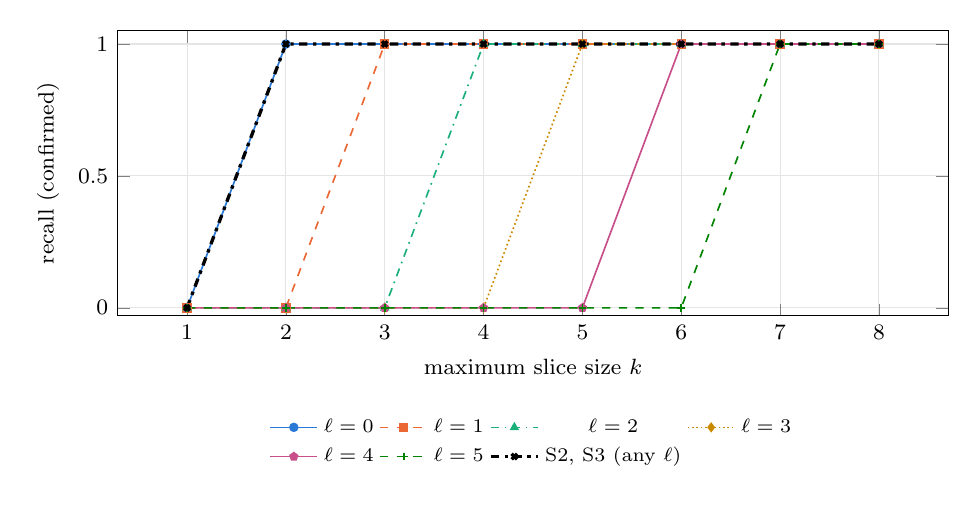
\begin{tikzpicture}\begin{axis}[width=\columnwidth,height=5.2cm,xlabel={maximum slice size $k$},ylabel={recall (confirmed)},xtick={1,2,3,4,5,6,7,8},ymin=-0.03,ymax=1.05,grid=major,grid style={gray!20},legend columns=4,legend style={at={(0.5,-0.32)},anchor=north,font=\scriptsize,draw=none,fill=none},tick label style={font=\footnotesize},label style={font=\footnotesize}]
\addplot[cA,semithick,solid,mark=*,mark size=1.4pt,mark options={solid}] coordinates {(1,0) (2,1) (3,1) (4,1) (5,1) (6,1) (7,1) (8,1)};
\addlegendentry{$\ell=0$}
\addplot[cB,semithick,dashed,mark=square*,mark size=1.4pt,mark options={solid}] coordinates {(1,0) (2,0) (3,1) (4,1) (5,1) (6,1) (7,1) (8,1)};
\addlegendentry{$\ell=1$}
\addplot[cC,semithick,dashdotted,mark=triangle*,mark size=1.4pt,mark options={solid}] coordinates {(1,0) (2,0) (3,0) (4,1) (5,1) (6,1) (7,1) (8,1)};
\addlegendentry{$\ell=2$}
\addplot[cD,semithick,densely dotted,mark=diamond*,mark size=1.4pt,mark options={solid}] coordinates {(1,0) (2,0) (3,0) (4,0) (5,1) (6,1) (7,1) (8,1)};
\addlegendentry{$\ell=3$}
\addplot[cE,semithick,solid,mark=pentagon*,mark size=1.4pt,mark options={solid}] coordinates {(1,0) (2,0) (3,0) (4,0) (5,0) (6,1) (7,1) (8,1)};
\addlegendentry{$\ell=4$}
\addplot[cF,semithick,dashed,mark=+,mark size=1.4pt,mark options={solid}] coordinates {(1,0) (2,0) (3,0) (4,0) (5,0) (6,0) (7,1) (8,1)};
\addlegendentry{$\ell=5$}
\addplot[black,very thick,dashdotted,mark=x,mark size=1.4pt,mark options={solid}] coordinates {(1,0) (2,1) (3,1) (4,1) (5,1) (6,1) (7,1) (8,1)};
\addlegendentry{S2, S3 (any $\ell$)}
\end{axis}\end{tikzpicture}}
\newcommand{\figEvolution}{%
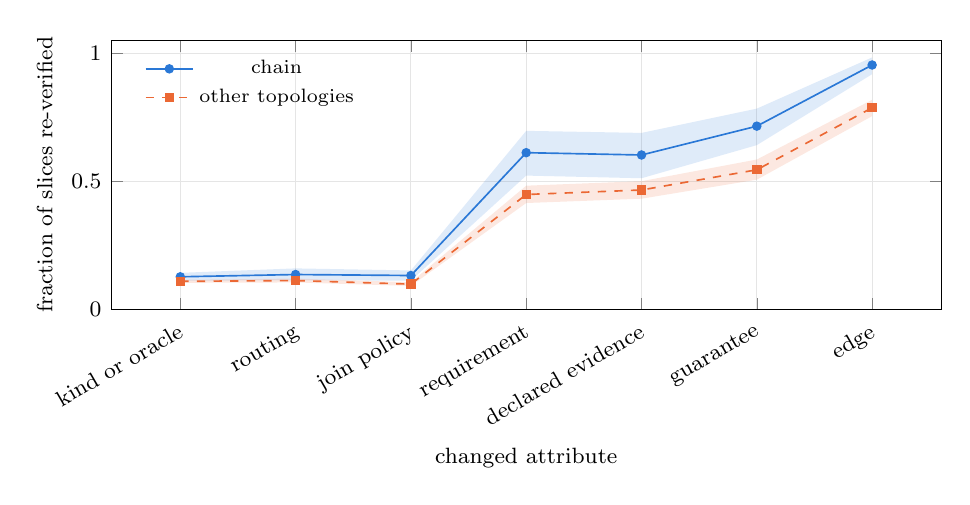
\begin{tikzpicture}\begin{axis}[width=\columnwidth,height=5cm,ymin=0,ymax=1.05,xtick={0,1,2,3,4,5,6},xticklabels={kind or oracle,routing,join policy,requirement,declared evidence,guarantee,edge},x tick label style={rotate=30,anchor=north east,font=\footnotesize},xlabel={changed attribute},ylabel={fraction of slices re-verified},grid=major,grid style={gray!20},legend pos=north west,legend style={font=\scriptsize,draw=none,fill=none},tick label style={font=\footnotesize},label style={font=\footnotesize}]
\addplot[fill=cA,fill opacity=0.15,draw=none,forget plot] coordinates {(0,0.112803) (1,0.113636) (2,0.112857) (3,0.522376) (4,0.512022) (5,0.641209) (6,0.918016) (6,0.983502) (5,0.783629) (4,0.688901) (3,0.696935) (2,0.152374) (1,0.160421) (0,0.143045)} -- cycle;
\addplot[cA,semithick,solid,mark=*,mark size=1.4pt,mark options={solid}] coordinates {(0,0.127657) (1,0.136491) (2,0.132616) (3,0.611777) (4,0.602782) (5,0.715277) (6,0.953787)};
\addlegendentry{chain}
\addplot[fill=cB,fill opacity=0.15,draw=none,forget plot] coordinates {(0,0.104038) (1,0.10562) (2,0.0919978) (3,0.415406) (4,0.432262) (5,0.506421) (6,0.754439) (6,0.818133) (5,0.585189) (4,0.500546) (3,0.483057) (2,0.10622) (1,0.120821) (0,0.115724)} -- cycle;
\addplot[cB,semithick,dashed,mark=square*,mark size=1.4pt,mark options={solid}] coordinates {(0,0.109813) (1,0.113022) (2,0.0989767) (3,0.448614) (4,0.466247) (5,0.545069) (6,0.78703)};
\addlegendentry{other topologies}
\end{axis}\end{tikzpicture}}
\newcommand{\figScalability}{%
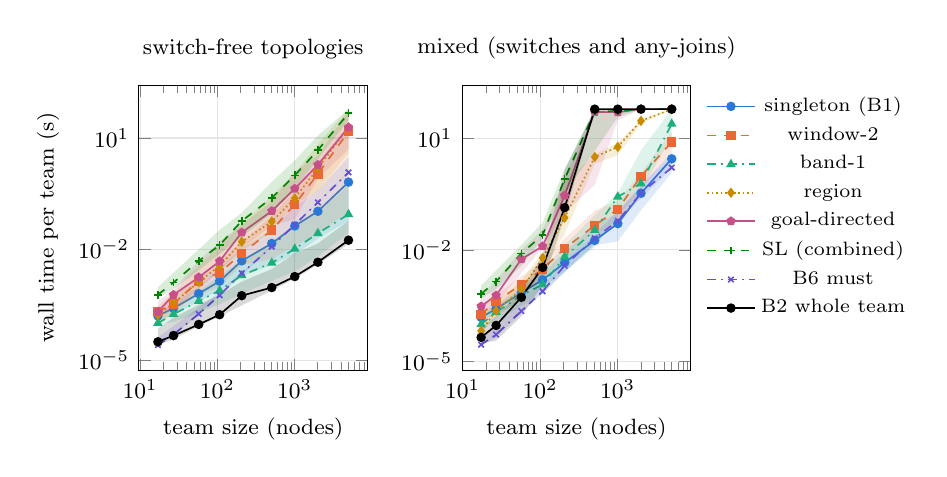
\begin{tikzpicture}
\begin{axis}[width=0.37\textwidth,height=5.2cm,xmode=log,ymode=log,xlabel={team size (nodes)},title={switch-free topologies},grid=major,grid style={gray!20},tick label style={font=\footnotesize},label style={font=\footnotesize},title style={font=\footnotesize},ylabel={wall time per team (s)},name=left]
\addplot[fill=cA,fill opacity=0.15,draw=none,forget plot] coordinates {(16.9667,0.000120048) (27.0333,0.000166955) (57.3333,0.000392596) (106.967,0.000777994) (207.033,0.0018467) (507.1,0.00374541) (1007.23,0.00716551) (2007.03,0.0194066) (5007.3,0.0578473) (5007.3,3.02781) (2007.03,0.387911) (1007.23,0.139894) (507.1,0.0327347) (207.033,0.0105312) (106.967,0.00300478) (57.3333,0.000974985) (27.0333,0.000349333) (16.9667,0.000188046)} -- cycle;
\addplot[cA,semithick,solid,mark=*,mark size=1.4pt,mark options={solid}] coordinates {(16.9667,0.00015729) (27.0333,0.000254816) (57.3333,0.000628252) (106.967,0.00136612) (207.033,0.00483464) (507.1,0.0142064) (1007.23,0.0422141) (2007.03,0.105046) (5007.3,0.643768)};
\addplot[fill=cB,fill opacity=0.15,draw=none,forget plot] coordinates {(16.9667,0.000143819) (27.0333,0.000237676) (57.3333,0.000582966) (106.967,0.000980023) (207.033,0.00371475) (507.1,0.00537092) (1007.23,0.0123311) (2007.03,0.0270928) (5007.3,0.10103) (5007.3,23.8108) (2007.03,2.23127) (1007.23,0.386551) (507.1,0.0793982) (207.033,0.0149007) (106.967,0.00483241) (57.3333,0.00186661) (27.0333,0.000533351) (16.9667,0.000250479)} -- cycle;
\addplot[cB,semithick,dashed,mark=square*,mark size=1.4pt,mark options={solid}] coordinates {(16.9667,0.00020609) (27.0333,0.000334446) (57.3333,0.00139132) (106.967,0.00229154) (207.033,0.00765147) (507.1,0.0324548) (1007.23,0.161023) (2007.03,1.07588) (5007.3,14.9045)};
\addplot[fill=cC,fill opacity=0.15,draw=none,forget plot] coordinates {(16.9667,8.9753e-05) (27.0333,0.000108453) (57.3333,0.00019363) (106.967,0.00032679) (207.033,0.000623552) (507.1,0.00139833) (1007.23,0.00247237) (2007.03,0.00642686) (5007.3,0.0271199) (5007.3,0.536141) (2007.03,0.0972302) (1007.23,0.0428923) (507.1,0.0148582) (207.033,0.00503602) (106.967,0.0019189) (57.3333,0.000736984) (27.0333,0.000254508) (16.9667,0.000142563)} -- cycle;
\addplot[cC,semithick,dashdotted,mark=triangle*,mark size=1.4pt,mark options={solid}] coordinates {(16.9667,0.000100853) (27.0333,0.000175682) (57.3333,0.00039418) (106.967,0.000763926) (207.033,0.00195937) (507.1,0.00425397) (1007.23,0.0101893) (2007.03,0.0267877) (5007.3,0.0869969)};
\addplot[fill=cD,fill opacity=0.15,draw=none,forget plot] coordinates {(16.9667,9.6209e-05) (27.0333,0.000169667) (57.3333,0.000863256) (106.967,0.00265774) (207.033,0.00855539) (507.1,0.0310307) (1007.23,0.164068) (2007.03,0.377455) (5007.3,3.92327) (5007.3,60) (2007.03,6.76566) (1007.23,1.11881) (507.1,0.269365) (207.033,0.0478197) (106.967,0.0118438) (57.3333,0.00368151) (27.0333,0.000676314) (16.9667,0.000290075)} -- cycle;
\addplot[cD,semithick,densely dotted,mark=diamond*,mark size=1.4pt,mark options={solid}] coordinates {(16.9667,0.000164979) (27.0333,0.000350669) (57.3333,0.00130771) (106.967,0.00351796) (207.033,0.0159012) (507.1,0.0558113) (1007.23,0.23423) (2007.03,1.52556) (5007.3,19.4435)};
\addplot[fill=cE,fill opacity=0.15,draw=none,forget plot] coordinates {(16.9667,0.000144204) (27.0333,0.000253528) (57.3333,0.000823454) (106.967,0.00263922) (207.033,0.0101432) (507.1,0.043934) (1007.23,0.063031) (2007.03,0.806436) (5007.3,4.99308) (5007.3,54.4165) (2007.03,3.32442) (1007.23,1.2496) (507.1,0.19275) (207.033,0.0458144) (106.967,0.0157522) (57.3333,0.00493797) (27.0333,0.000808794) (16.9667,0.000394608)} -- cycle;
\addplot[cE,semithick,solid,mark=pentagon*,mark size=1.4pt,mark options={solid}] coordinates {(16.9667,0.000202442) (27.0333,0.000584957) (57.3333,0.00174012) (106.967,0.004708) (207.033,0.0280934) (507.1,0.10683) (1007.23,0.427459) (2007.03,1.88829) (5007.3,19.3022)};
\addplot[fill=cF,fill opacity=0.15,draw=none,forget plot] coordinates {(16.9667,0.000493569) (27.0333,0.000835017) (57.3333,0.00269003) (106.967,0.00746663) (207.033,0.0218094) (507.1,0.0919288) (1007.23,0.445087) (2007.03,2.65424) (5007.3,30.4298) (5007.3,60) (2007.03,11.6051) (1007.23,2.48253) (507.1,0.651728) (207.033,0.0955993) (106.967,0.0329586) (57.3333,0.00981074) (27.0333,0.00230517) (16.9667,0.000941222)} -- cycle;
\addplot[cF,semithick,dashed,mark=+,mark size=1.4pt,mark options={solid}] coordinates {(16.9667,0.000588061) (27.0333,0.00125559) (57.3333,0.00478189) (106.967,0.0128729) (207.033,0.0575003) (507.1,0.241591) (1007.23,0.979675) (2007.03,4.69068) (5007.3,46.8205)};
\addplot[fill=cG,fill opacity=0.15,draw=none,forget plot] coordinates {(16.9667,2.3415e-05) (27.0333,4.62462e-05) (57.3333,0.000173514) (106.967,0.000560214) (207.033,0.00195677) (507.1,0.0115982) (1007.23,0.0454798) (2007.03,0.180767) (5007.3,1.16502) (5007.3,1.19979) (2007.03,0.185294) (1007.23,0.0478615) (507.1,0.0123403) (207.033,0.00239195) (106.967,0.000702508) (57.3333,0.000265055) (27.0333,8.4106e-05) (16.9667,4.1019e-05)} -- cycle;
\addplot[cG,semithick,dashdotted,mark=x,mark size=1.4pt,mark options={solid}] coordinates {(16.9667,2.5735e-05) (27.0333,4.9462e-05) (57.3333,0.000178498) (106.967,0.000567941) (207.033,0.00223053) (507.1,0.0116609) (1007.23,0.0458937) (2007.03,0.182258) (5007.3,1.17676)};
\addplot[fill=black,fill opacity=0.15,draw=none,forget plot] coordinates {(16.9667,2.6099e-05) (27.0333,3.6711e-05) (57.3333,8.2781e-05) (106.967,0.000150603) (207.033,0.000303072) (507.1,0.000762835) (1007.23,0.0016025) (2007.03,0.0038419) (5007.3,0.0139452) (5007.3,0.0578302) (2007.03,0.0142184) (1007.23,0.00760897) (507.1,0.00289576) (207.033,0.00132662) (106.967,0.000579933) (57.3333,0.000313914) (27.0333,0.000140819) (16.9667,7.19092e-05)} -- cycle;
\addplot[black,semithick,solid,mark=*,mark size=1.4pt,mark options={solid}] coordinates {(16.9667,3.1519e-05) (27.0333,4.6359e-05) (57.3333,9.2805e-05) (106.967,0.000170171) (207.033,0.000555448) (507.1,0.00091836) (1007.23,0.00181892) (2007.03,0.00443092) (5007.3,0.0174429)};
\end{axis}
\begin{axis}[width=0.37\textwidth,height=5.2cm,xmode=log,ymode=log,xlabel={team size (nodes)},title={mixed (switches and any-joins)},grid=major,grid style={gray!20},tick label style={font=\footnotesize},label style={font=\footnotesize},title style={font=\footnotesize},legend pos=outer north east,legend style={font=\scriptsize,draw=none,fill=none},at={(left.east)},anchor=west,xshift=1.2cm]
\addplot[fill=cA,fill opacity=0.15,draw=none,forget plot] coordinates {(17.3,0.000121572) (27,0.000185146) (57.2,0.000431122) (107.7,0.00100008) (207.4,0.00263949) (507.2,0.0134414) (1006.7,0.0169017) (2006.8,0.116719) (5007.1,1.16072) (5007.1,4.33078) (2006.8,0.491884) (1006.7,0.0959776) (507.2,0.0484253) (207.4,0.00867031) (107.7,0.00234411) (57.2,0.00105627) (27,0.000331573) (17.3,0.000213033)} -- cycle;
\addplot[cA,semithick,solid,mark=*,mark size=1.4pt,mark options={solid}] coordinates {(17.3,0.000154091) (27,0.000261128) (57.2,0.000711993) (107.7,0.00156663) (207.4,0.00455263) (507.2,0.0180262) (1006.7,0.0507408) (2006.8,0.33142) (5007.1,2.78201)};
\addlegendentry{singleton (B1)}
\addplot[fill=cB,fill opacity=0.15,draw=none,forget plot] coordinates {(17.3,0.000176107) (27,0.000265712) (57.2,0.000640003) (107.7,0.00171463) (207.4,0.00541682) (507.2,0.0290629) (1006.7,0.0457185) (2006.8,0.407786) (5007.1,4.4199) (5007.1,14.7143) (2006.8,1.1598) (1006.7,0.210604) (507.2,0.112138) (207.4,0.0202843) (107.7,0.00495972) (57.2,0.00196482) (27,0.000617908) (17.3,0.000334161)} -- cycle;
\addplot[cB,semithick,dashed,mark=square*,mark size=1.4pt,mark options={solid}] coordinates {(17.3,0.000187954) (27,0.000412674) (57.2,0.00117127) (107.7,0.00303593) (207.4,0.0109777) (507.2,0.0451589) (1006.7,0.122926) (2006.8,0.942846) (5007.1,7.91836)};
\addlegendentry{window-2}
\addplot[fill=cC,fill opacity=0.15,draw=none,forget plot] coordinates {(17.3,8.4941e-05) (27,0.000121816) (57.2,0.00032031) (107.7,0.000655959) (207.4,0.00260104) (507.2,0.0119245) (1006.7,0.0881359) (2006.8,0.39004) (5007.1,11.0832) (5007.1,60) (2006.8,4.67392) (1006.7,0.327819) (507.2,0.0860516) (207.4,0.0133196) (107.7,0.00263147) (57.2,0.000860577) (27,0.000304634) (17.3,0.000172126)} -- cycle;
\addplot[cC,semithick,dashdotted,mark=triangle*,mark size=1.4pt,mark options={solid}] coordinates {(17.3,0.000100325) (27,0.000213313) (57.2,0.000598636) (107.7,0.00117523) (207.4,0.00651923) (507.2,0.0338071) (1006.7,0.267442) (2006.8,0.601596) (5007.1,24.1802)};
\addlegendentry{band-1}
\addplot[fill=cD,fill opacity=0.15,draw=none,forget plot] coordinates {(17.3,5.7502e-05) (27,0.000154199) (57.2,0.000488284) (107.7,0.0027201) (207.4,0.0268087) (507.2,2.05295) (1006.7,3.47144) (2006.8,24.5861) (5007.1,60) (5007.1,60) (2006.8,31.5973) (1006.7,7.36887) (507.2,3.71785) (207.4,0.651038) (107.7,0.00854709) (57.2,0.00147837) (27,0.000413974) (17.3,0.000163522)} -- cycle;
\addplot[cD,semithick,densely dotted,mark=diamond*,mark size=1.4pt,mark options={solid}] coordinates {(17.3,6.7278e-05) (27,0.000235224) (57.2,0.000862861) (107.7,0.0060858) (207.4,0.0730611) (507.2,3.12323) (1006.7,5.81045) (2006.8,29.0479) (5007.1,60)};
\addlegendentry{region}
\addplot[fill=cE,fill opacity=0.15,draw=none,forget plot] coordinates {(17.3,0.000194342) (27,0.000334557) (57.2,0.00237598) (107.7,0.0117868) (207.4,0.103844) (507.2,0.551529) (1006.7,30.2061) (2006.8,60) (5007.1,60) (5007.1,60) (2006.8,60) (1006.7,60) (507.2,60) (207.4,0.803908) (107.7,0.0351231) (57.2,0.00965705) (27,0.00152338) (17.3,0.000581985)} -- cycle;
\addplot[cE,semithick,solid,mark=pentagon*,mark size=1.4pt,mark options={solid}] coordinates {(17.3,0.000306102) (27,0.000600917) (57.2,0.00562597) (107.7,0.0125803) (207.4,0.287989) (507.2,50.4143) (1006.7,49.7176) (2006.8,60) (5007.1,60)};
\addlegendentry{goal-directed}
\addplot[fill=cF,fill opacity=0.15,draw=none,forget plot] coordinates {(17.3,0.000493076) (27,0.000879115) (57.2,0.00370001) (107.7,0.0205619) (207.4,0.342036) (507.2,4.56517) (1006.7,36.6745) (2006.8,60) (5007.1,60) (5007.1,60) (2006.8,60) (1006.7,60) (507.2,60) (207.4,1.50041) (107.7,0.0546107) (57.2,0.0135201) (27,0.00280253) (17.3,0.00109144)} -- cycle;
\addplot[cF,semithick,dashed,mark=+,mark size=1.4pt,mark options={solid}] coordinates {(17.3,0.000666011) (27,0.00140645) (57.2,0.00804486) (107.7,0.0250347) (207.4,0.804673) (507.2,52.428) (1006.7,53.5691) (2006.8,60) (5007.1,60)};
\addlegendentry{SL (combined)}
\addplot[fill=cG,fill opacity=0.15,draw=none,forget plot] coordinates {(17.3,2.5399e-05) (27,4.5186e-05) (57.2,0.000201634) (107.7,0.000697594) (207.4,0.00249952) (507.2,0.014638) (1006.7,0.0566756) (2006.8,0.244117) (5007.1,1.58398) (5007.1,3.65541) (2006.8,0.536709) (1006.7,0.110983) (507.2,0.0262924) (207.4,0.00557297) (107.7,0.00105899) (57.2,0.00042075) (27,9.6757e-05) (17.3,4.57423e-05)} -- cycle;
\addplot[cG,semithick,dashdotted,mark=x,mark size=1.4pt,mark options={solid}] coordinates {(17.3,2.85675e-05) (27,5.3494e-05) (57.2,0.000227353) (107.7,0.000775159) (207.4,0.00378522) (507.2,0.0205932) (1006.7,0.060237) (2006.8,0.336663) (5007.1,1.62042)};
\addlegendentry{B6 must}
\addplot[fill=black,fill opacity=0.15,draw=none,forget plot] coordinates {(17.3,3.20547e-05) (27,3.6695e-05) (57.2,0.000163667) (107.7,0.00115923) (207.4,0.0792335) (507.2,56.1834) (1006.7,60) (2006.8,60) (5007.1,60) (5007.1,60) (2006.8,60) (1006.7,60) (507.2,60) (207.4,1.38403) (107.7,0.00703874) (57.2,0.000782739) (27,0.00016447) (17.3,8.23137e-05)} -- cycle;
\addplot[black,semithick,solid,mark=*,mark size=1.4pt,mark options={solid}] coordinates {(17.3,4.49345e-05) (27,9.3925e-05) (57.2,0.000533815) (107.7,0.00338702) (207.4,0.136157) (507.2,60) (1006.7,60) (2006.8,60) (5007.1,60)};
\addlegendentry{B2 whole team}
\end{axis}
\end{tikzpicture}}
\newcommand{\figTeaser}{%
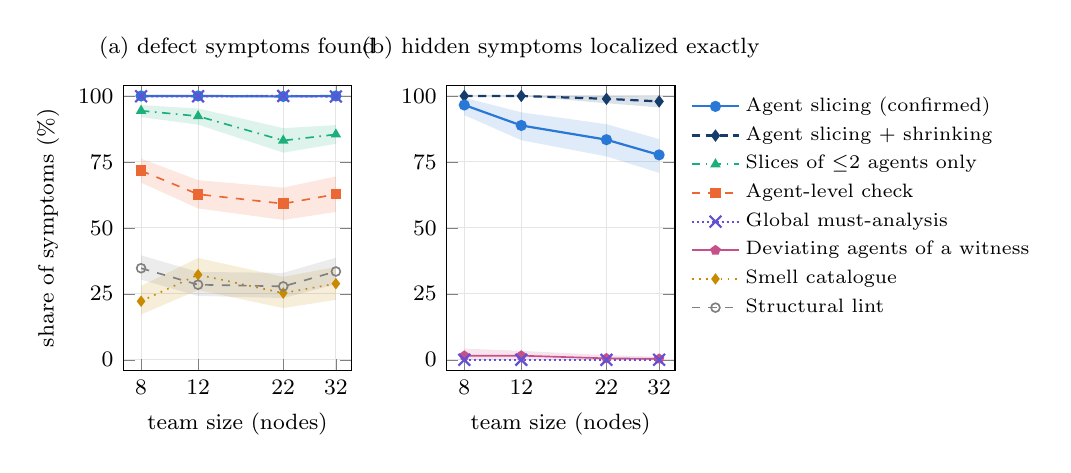
\begin{tikzpicture}
\begin{axis}[width=0.37\textwidth,height=5.2cm,xmode=log,log basis x=2,xtick={8,12,22,32},xticklabels={8,12,22,32},xmin=7.04,xmax=35.84,ymin=-4,ymax=104,ytick={0,25,50,75,100},xlabel={team size (nodes)},grid=major,grid style={gray!20},tick label style={font=\footnotesize},label style={font=\footnotesize},title style={font=\footnotesize},title={(a) defect symptoms found},ylabel={share of symptoms (\%)},name=left]
\addplot[fill=cA,fill opacity=0.15,draw=none,forget plot] coordinates {(8,100) (12,100) (22,99.4371) (32,100) (32,100) (22,100) (12,100) (8,100)} -- cycle;
\addplot[mark size=1.6pt,cA,thick,solid,mark=*,mark options={solid},forget plot] coordinates {(8,100) (12,100) (22,99.8193) (32,100)};
\addplot[fill=cC,fill opacity=0.15,draw=none,forget plot] coordinates {(8,91.9832) (12,89.1408) (22,78.5073) (32,81.8669) (32,88.948) (22,87.805) (12,95.2619) (8,96.5186)} -- cycle;
\addplot[mark size=1.6pt,cC,semithick,dashdotted,mark=triangle*,mark options={solid},forget plot] coordinates {(8,94.3966) (12,92.3429) (22,83.1075) (32,85.4145)};
\addplot[fill=cB,fill opacity=0.15,draw=none,forget plot] coordinates {(8,67.1161) (12,57.3767) (22,53) (32,56.0377) (32,69.5009) (22,65.2737) (12,68.1005) (8,76.2583)} -- cycle;
\addplot[mark size=1.6pt,cB,semithick,dashed,mark=square*,mark options={solid},forget plot] coordinates {(8,71.6595) (12,62.7429) (22,59.1689) (32,62.7492)};
\addplot[fill=cD,fill opacity=0.15,draw=none,forget plot] coordinates {(8,17.1734) (12,26.4341) (22,19.5971) (32,22.7219) (32,35.1872) (22,31.4382) (12,38.5899) (8,28.0188)} -- cycle;
\addplot[mark size=1.6pt,cD,semithick,dotted,mark=diamond*,mark options={solid},forget plot] coordinates {(8,22.1983) (12,32.2286) (22,25.2936) (32,28.8562)};
\addplot[fill=gray,fill opacity=0.15,draw=none,forget plot] coordinates {(8,30.3534) (12,24.193) (22,23.4007) (32,28.6427) (32,38.6839) (22,32.9529) (12,33.2909) (8,39.6147)} -- cycle;
\addplot[mark size=1.6pt,gray,semithick,dashed,mark=o,mark options={solid},forget plot] coordinates {(8,34.6983) (12,28.4571) (22,27.8229) (32,33.4732)};
\addplot[fill=cG,fill opacity=0.15,draw=none,forget plot] coordinates {(8,99.6458) (12,99.6324) (22,100) (32,99.4344) (32,100) (22,100) (12,100) (8,100)} -- cycle;
\addplot[mark size=1.6pt,cG,thick,densely dotted,mark=x,mark size=3pt,mark options={solid},forget plot] coordinates {(8,99.8922) (12,99.8857) (22,100) (32,99.7901)};
\end{axis}
\begin{axis}[width=0.37\textwidth,height=5.2cm,xmode=log,log basis x=2,xtick={8,12,22,32},xticklabels={8,12,22,32},xmin=7.04,xmax=35.84,ymin=-4,ymax=104,ytick={0,25,50,75,100},xlabel={team size (nodes)},grid=major,grid style={gray!20},tick label style={font=\footnotesize},label style={font=\footnotesize},title style={font=\footnotesize},title={(b) hidden symptoms localized exactly},at={(left.east)},anchor=west,xshift=1.2cm,legend pos=outer north east,legend cell align=left,legend style={font=\scriptsize,draw=none,fill=none}]
\addlegendimage{mark size=1.6pt,cA,thick,solid,mark=*,mark options={solid}}\addlegendentry{Agent slicing (confirmed)}
\addlegendimage{mark size=1.6pt,cA!50!black,thick,densely dashed,mark=diamond*,mark options={solid}}\addlegendentry{Agent slicing + shrinking}
\addlegendimage{mark size=1.6pt,cC,semithick,dashdotted,mark=triangle*,mark options={solid}}\addlegendentry{Slices of $\le$2 agents only}
\addlegendimage{mark size=1.6pt,cB,semithick,dashed,mark=square*,mark options={solid}}\addlegendentry{Agent-level check}
\addlegendimage{mark size=1.6pt,cG,thick,densely dotted,mark=x,mark size=3pt,mark options={solid}}\addlegendentry{Global must-analysis}
\addlegendimage{mark size=1.6pt,cE,semithick,solid,mark=pentagon*,mark options={solid}}\addlegendentry{Deviating agents of a witness}
\addlegendimage{mark size=1.6pt,cD,semithick,dotted,mark=diamond*,mark options={solid}}\addlegendentry{Smell catalogue}
\addlegendimage{mark size=1.6pt,gray,semithick,dashed,mark=o,mark options={solid}}\addlegendentry{Structural lint}
\addplot[fill=cA!50!black,fill opacity=0.15,draw=none,forget plot] coordinates {(8,100) (12,100) (22,97.2642) (32,95.6693) (32,99.6645) (22,100) (12,100) (8,100)} -- cycle;
\addplot[mark size=1.6pt,cA!50!black,thick,densely dashed,mark=diamond*,mark options={solid},forget plot] coordinates {(8,100) (12,100) (22,98.913) (32,97.9381)};
\addplot[fill=cA,fill opacity=0.15,draw=none,forget plot] coordinates {(8,92.7417) (12,83.2351) (22,77.1047) (32,70.863) (32,83.6513) (22,89.2944) (12,93.8054) (8,99.3468)} -- cycle;
\addplot[mark size=1.6pt,cA,thick,solid,mark=*,mark options={solid},forget plot] coordinates {(8,96.5779) (12,88.8199) (22,83.4239) (32,77.6632)};
\addplot[fill=cE,fill opacity=0.15,draw=none,forget plot] coordinates {(8,0) (12,0.293255) (22,0) (32,0) (32,1.14943) (22,1.77528) (12,3.37838) (8,4.23753)} -- cycle;
\addplot[mark size=1.6pt,cE,semithick,solid,mark=pentagon*,mark options={solid},forget plot] coordinates {(8,1.52091) (12,1.5528) (22,0.543478) (32,0.343643)};
\addplot[fill=cG,fill opacity=0.15,draw=none,forget plot] coordinates {(8,0) (12,0) (22,0) (32,0) (32,0) (22,0) (12,0) (8,0)} -- cycle;
\addplot[mark size=1.6pt,cG,thick,densely dotted,mark=x,mark size=3pt,mark options={solid},forget plot] coordinates {(8,0) (12,0) (22,0) (32,0)};
\end{axis}
\end{tikzpicture}}
\newcommand{\resMutBSixFalseRateNOneZero}{4.3\%}
\newcommand{\resMutBSixFalseRateNSix}{1.4\%}
\newcommand{\resMutBSixFalseRateNThreeZero}{4.4\%}
\newcommand{\resMutBSixFalseRateNTwoZero}{2.9\%}
\newcommand{\resMutOpAddRequirementALSilent}{25}
\newcommand{\resMutOpAddRequirementHidden}{31.9\%}
\newcommand{\resMutOpAddRequirementSingleHidden}{28.0\%}
\newcommand{\resMutOpAddRequirementSingleTeams}{109}
\newcommand{\resMutOpAddRequirementSingleUnclean}{102}
\newcommand{\resMutOpAddRequirementTeams}{548}
\newcommand{\resMutOpAddRequirementUnclean}{501}
\newcommand{\resMutOpAddRequirementUncleanShare}{91.4\%}
\newcommand{\resMutOpDropGuaranteeALSilent}{35}
\newcommand{\resMutOpDropGuaranteeHidden}{24.2\%}
\newcommand{\resMutOpDropGuaranteeSingleHidden}{7.3\%}
\newcommand{\resMutOpDropGuaranteeSingleTeams}{80}
\newcommand{\resMutOpDropGuaranteeSingleUnclean}{71}
\newcommand{\resMutOpDropGuaranteeTeams}{511}
\newcommand{\resMutOpDropGuaranteeUnclean}{445}
\newcommand{\resMutOpDropGuaranteeUncleanShare}{87.1\%}
\newcommand{\resMutOpForkToSwitchALSilent}{14}
\newcommand{\resMutOpForkToSwitchHidden}{24.7\%}
\newcommand{\resMutOpForkToSwitchSingleTeams}{65}
\newcommand{\resMutOpForkToSwitchSingleUnclean}{0}
\newcommand{\resMutOpForkToSwitchTeams}{404}
\newcommand{\resMutOpForkToSwitchUnclean}{138}
\newcommand{\resMutOpForkToSwitchUncleanShare}{34.2\%}
\newcommand{\resMutOpGateToAgentALSilent}{56}
\newcommand{\resMutOpGateToAgentHidden}{34.2\%}
\newcommand{\resMutOpGateToAgentSingleHidden}{12.7\%}
\newcommand{\resMutOpGateToAgentSingleTeams}{90}
\newcommand{\resMutOpGateToAgentSingleUnclean}{79}
\newcommand{\resMutOpGateToAgentTeams}{495}
\newcommand{\resMutOpGateToAgentUnclean}{415}
\newcommand{\resMutOpGateToAgentUncleanShare}{83.8\%}
\newcommand{\resMutOpRelaxJoinALSilent}{157}
\newcommand{\resMutOpRelaxJoinHidden}{67.1\%}
\newcommand{\resMutOpRelaxJoinSingleHidden}{86.2\%}
\newcommand{\resMutOpRelaxJoinSingleTeams}{80}
\newcommand{\resMutOpRelaxJoinSingleUnclean}{78}
\newcommand{\resMutOpRelaxJoinTeams}{403}
\newcommand{\resMutOpRelaxJoinUnclean}{369}
\newcommand{\resMutOpRelaxJoinUncleanShare}{91.6\%}
\newcommand{\resMutOpRemoveEdgeALSilent}{13}
\newcommand{\resMutOpRemoveEdgeHidden}{22.6\%}
\newcommand{\resMutOpRemoveEdgeSingleHidden}{11.1\%}
\newcommand{\resMutOpRemoveEdgeSingleTeams}{19}
\newcommand{\resMutOpRemoveEdgeSingleUnclean}{17}
\newcommand{\resMutOpRemoveEdgeTeams}{109}
\newcommand{\resMutOpRemoveEdgeUnclean}{94}
\newcommand{\resMutOpRemoveEdgeUncleanShare}{86.2\%}
\newcommand{\resMutOpShareOracleALSilent}{74}
\newcommand{\resMutOpShareOracleHidden}{36.3\%}
\newcommand{\resMutOpShareOracleSingleHidden}{10.9\%}
\newcommand{\resMutOpShareOracleSingleTeams}{117}
\newcommand{\resMutOpShareOracleSingleUnclean}{101}
\newcommand{\resMutOpShareOracleTeams}{565}
\newcommand{\resMutOpShareOracleUnclean}{461}
\newcommand{\resMutOpShareOracleUncleanShare}{81.6\%}
\newcommand{\resMutSingleChangeTeams}{560}
\newcommand{\resMutComboTeams}{1{,}120}
\newcommand{\resMutOpAddRequirementComboHidden}{32.6\%}
\newcommand{\resMutOpAddRequirementComboKeys}{1{,}632}
\newcommand{\resMutOpDropGuaranteeComboHidden}{26.1\%}
\newcommand{\resMutOpDropGuaranteeComboKeys}{1{,}350}
\newcommand{\resMutOpForkToSwitchComboHidden}{24.7\%}
\newcommand{\resMutOpForkToSwitchComboKeys}{377}
\newcommand{\resMutOpGateToAgentComboHidden}{36.0\%}
\newcommand{\resMutOpGateToAgentComboKeys}{990}
\newcommand{\resMutOpRelaxJoinComboHidden}{63.4\%}
\newcommand{\resMutOpRelaxJoinComboKeys}{1{,}100}
\newcommand{\resMutOpRemoveEdgeComboHidden}{24.1\%}
\newcommand{\resMutOpRemoveEdgeComboKeys}{203}
\newcommand{\resMutOpShareOracleComboHidden}{39.0\%}
\newcommand{\resMutOpShareOracleComboKeys}{970}
\newcommand{\figDepthByOp}{%
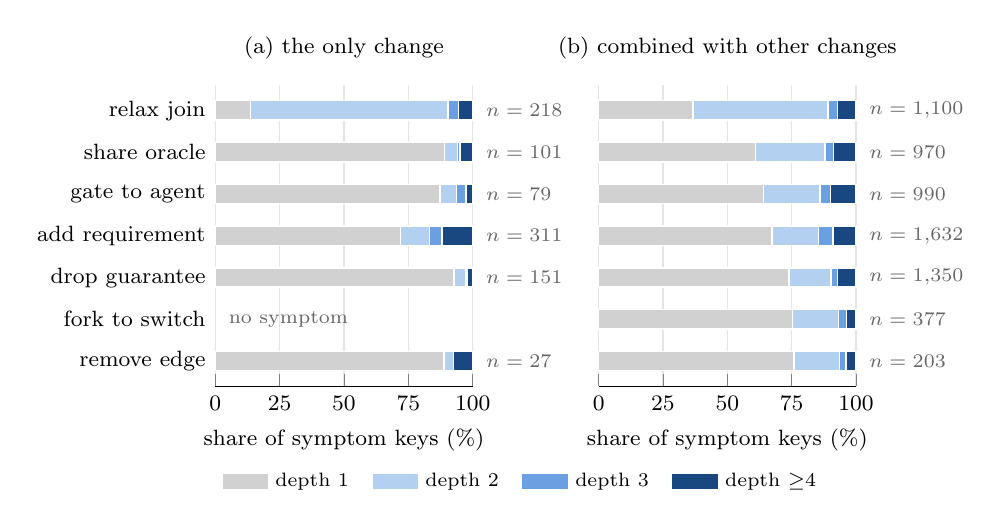
\begin{tikzpicture}
\begin{axis}[xbar stacked,bar width=7pt,width=0.40\textwidth,height=5.4cm,xmin=0,xmax=100,ytick={0,1,2,3,4,5,6},ymin=-0.6,ymax=6.6,xtick={0,25,50,75,100},xlabel={share of symptom keys (\%)},axis y line*=left,axis x line*=bottom,xmajorgrids,grid style={gray!20},y axis line style={draw=none},ytick style={draw=none},tick label style={font=\footnotesize},label style={font=\footnotesize},title style={font=\footnotesize},title={(a) the only change},clip=false,yticklabels={remove edge,fork to switch,drop guarantee,add requirement,gate to agent,share oracle,relax join},name=left]
\addplot[fill=black!18,draw=white,line width=0.5pt] coordinates {(88.89,0) (0,1) (92.72,2) (72.03,3) (87.34,4) (89.11,5) (13.76,6)};
\addplot[fill=cA!35,draw=white,line width=0.5pt] coordinates {(3.704,0) (0,1) (4.636,2) (11.25,3) (6.329,4) (4.95,5) (76.61,6)};
\addplot[fill=cA!70,draw=white,line width=0.5pt] coordinates {(0,0) (0,1) (0.6623,2) (4.823,3) (3.797,4) (0.9901,5) (4.128,6)};
\addplot[fill=cA!60!black,draw=white,line width=0.5pt] coordinates {(7.407,0) (0,1) (1.987,2) (11.9,3) (2.532,4) (4.95,5) (5.505,6)};
\node[font=\scriptsize,text=black!60,anchor=west] at (axis cs:100,0) {\,$n=27$};
\node[font=\scriptsize,text=black!60,anchor=west] at (axis cs:0,1) {\,no symptom};
\node[font=\scriptsize,text=black!60,anchor=west] at (axis cs:100,2) {\,$n=151$};
\node[font=\scriptsize,text=black!60,anchor=west] at (axis cs:100,3) {\,$n=311$};
\node[font=\scriptsize,text=black!60,anchor=west] at (axis cs:100,4) {\,$n=79$};
\node[font=\scriptsize,text=black!60,anchor=west] at (axis cs:100,5) {\,$n=101$};
\node[font=\scriptsize,text=black!60,anchor=west] at (axis cs:100,6) {\,$n=218$};
\end{axis}
\begin{axis}[xbar stacked,bar width=7pt,width=0.40\textwidth,height=5.4cm,xmin=0,xmax=100,ytick={0,1,2,3,4,5,6},ymin=-0.6,ymax=6.6,xtick={0,25,50,75,100},xlabel={share of symptom keys (\%)},axis y line*=left,axis x line*=bottom,xmajorgrids,grid style={gray!20},y axis line style={draw=none},ytick style={draw=none},tick label style={font=\footnotesize},label style={font=\footnotesize},title style={font=\footnotesize},title={(b) combined with other changes},clip=false,yticklabels={},at={(left.east)},anchor=west,xshift=1.6cm,area legend,legend columns=4,legend style={at={(-0.3,-0.25)},anchor=north,font=\scriptsize,draw=none,fill=none,/tikz/every even column/.append style={column sep=6pt}},legend cell align=left]
\addplot[fill=black!18,draw=white,line width=0.5pt] coordinates {(75.86,0) (75.33,1) (73.93,2) (67.4,3) (64.04,4) (61.03,5) (36.64,6)};
\addlegendentry{depth 1}
\addplot[fill=cA!35,draw=white,line width=0.5pt] coordinates {(17.73,0) (17.77,1) (16.37,2) (18.14,3) (21.92,4) (26.91,5) (52.45,6)};
\addlegendentry{depth 2}
\addplot[fill=cA!70,draw=white,line width=0.5pt] coordinates {(2.463,0) (3.183,1) (2.593,2) (5.453,3) (4.04,4) (3.299,5) (3.727,6)};
\addlegendentry{depth 3}
\addplot[fill=cA!60!black,draw=white,line width=0.5pt] coordinates {(3.941,0) (3.714,1) (7.111,2) (9.007,3) (10,4) (8.763,5) (7.182,6)};
\addlegendentry{depth $\ge$4}
\node[font=\scriptsize,text=black!60,anchor=west] at (axis cs:100,0) {\,$n=203$};
\node[font=\scriptsize,text=black!60,anchor=west] at (axis cs:100,1) {\,$n=377$};
\node[font=\scriptsize,text=black!60,anchor=west] at (axis cs:100,2) {\,$n=1{,}350$};
\node[font=\scriptsize,text=black!60,anchor=west] at (axis cs:100,3) {\,$n=1{,}632$};
\node[font=\scriptsize,text=black!60,anchor=west] at (axis cs:100,4) {\,$n=990$};
\node[font=\scriptsize,text=black!60,anchor=west] at (axis cs:100,5) {\,$n=970$};
\node[font=\scriptsize,text=black!60,anchor=west] at (axis cs:100,6) {\,$n=1{,}100$};
\end{axis}
\end{tikzpicture}}
\newcommand{\resEvoAllSlicesdecl}{0.0\%}
\newcommand{\resEvoAllSlicesedge}{41.4\%}
\newcommand{\resEvoAllSlicesgua}{6.6\%}
\newcommand{\resEvoAllSlicesjoin}{0.0\%}
\newcommand{\resEvoAllSliceskind}{0.0\%}
\newcommand{\resEvoAllSlicesreq}{0.0\%}
\newcommand{\resEvoAllSlicesroute}{0.0\%}
\newcommand{\resEvoFullMs}{3.6}
\newcommand{\resEvoIncMs}{1.9}
\newcommand{\resEvoMediandecl}{41.5\%}
\newcommand{\resEvoMedianedge}{96.6\%}
\newcommand{\resEvoMediangua}{56.6\%}
\newcommand{\resEvoMedianjoin}{9.4\%}
\newcommand{\resEvoMediankind}{10.2\%}
\newcommand{\resEvoMedianreq}{38.1\%}
\newcommand{\resEvoMedianroute}{10.7\%}
\newcommand{\resEvoSlicesNEightZero}{281}
\newcommand{\resEvoSlicesNFourZero}{145}
\newcommand{\resEvoSlicesNTwoZero}{78}
\newcommand{\resEvoSlowerdecl}{19.1\%}
\newcommand{\resEvoSloweredge}{66.6\%}
\newcommand{\resEvoSlowergua}{27.9\%}
\newcommand{\resEvoSlowerjoin}{0.0\%}
\newcommand{\resEvoSlowerkind}{0.2\%}
\newcommand{\resEvoSlowerreq}{16.1\%}
\newcommand{\resEvoSlowerroute}{0.4\%}
\newcommand{\resEvoSpeedupdecl}{1.4}
\newcommand{\resEvoSpeedupedge}{0.9}
\newcommand{\resEvoSpeedupgua}{1.2}
\newcommand{\resEvoSpeedupjoin}{3.4}
\newcommand{\resEvoSpeedupkind}{3.2}
\newcommand{\resEvoSpeedupreq}{1.4}
\newcommand{\resEvoSpeeduproute}{2.9}
\newcommand{\tabEvolutionDetail}{%
\multicolumn{13}{@{}l}{\textit{Node policy}}\\
\quad kind or oracle & $\{a\}$ & 465 & 11.3 & {\footnotesize[10.7, 11.8]} & 10.2 & 0.0 & 14.4 & 10.9 & 8.8 & 3.5 & 3.2 & 0.2 \\
\quad routing & $\{a\}$ & 258 & 11.6 & {\footnotesize[10.9, 12.3]} & 10.7 & 0.0 & 14.9 & 11.5 & 8.5 & 4.1 & 2.9 & 0.4 \\
\quad join policy & $\{a\}$ & 226 & 10.4 & {\footnotesize[9.7, 11.1]} & 9.4 & 0.0 & 12.9 & 10.1 & 8.2 & 3.3 & 3.4 & 0.0 \\
\addlinespace
\multicolumn{13}{@{}l}{\textit{Node contract}}\\
\quad requirement & $\anc^*(a)$ & 248 & 46.8 & {\footnotesize[43.6, 50.0]} & 38.1 & 0.0 & 52.1 & 47.5 & 42.2 & 4.6 & 1.4 & 16.1 \\
\quad declared evidence & $\anc^*(a)$ & 251 & 48.5 & {\footnotesize[45.2, 51.7]} & 41.5 & 0.0 & 54.5 & 47.6 & 41.5 & 3.0 & 1.4 & 19.1 \\
\quad guarantee & $\anc^*(Y)$ & 229 & 57.3 & {\footnotesize[53.6, 60.9]} & 56.6 & 6.6 & 60.4 & 53.7 & 57.2 & 3.8 & 1.2 & 27.9 \\
\addlinespace
\multicolumn{13}{@{}l}{\textit{Structure}}\\
\quad edge added or removed & $\anc^*(Y)$, both & 290 & 80.7 & {\footnotesize[77.7, 83.5]} & 96.6 & 41.4 & 84.7 & 85.3 & 71.8 & 3.1 & 0.9 & 66.6 \\
\midrule
All changes &  & 1{,}967 & 36.0 & {\footnotesize[34.6, 37.4]} & 21.7 & 6.9 & 41.5 & 34.5 & 32.1 & 3.6 & 1.9 & 17.6 \\}
\newcommand{\tabEvolutionTopology}{%
\multicolumn{9}{@{}l}{\textit{Node policy}}\\
\quad kind or oracle & 465 & 12.8 & 8.1 & 15.1 & 13.5 & 10.0 & 10.7 & 9.8 & 11.3 \\
\quad routing & 258 & 13.6 & 9.4 & 14.6 & 13.9 & 10.3 & 9.8 & 9.4 & 11.6 \\
\quad join policy & 226 & 13.3 & 7.9 & 11.9 & 11.0 & 9.6 & 8.2 & 10.4 & 10.4 \\
\addlinespace
\multicolumn{9}{@{}l}{\textit{Node contract}}\\
\quad requirement & 248 & 61.2 & 36.8 & 58.9 & 52.0 & 37.9 & 31.7 & 54.9 & 46.8 \\
\quad declared evidence & 251 & 60.3 & 29.4 & 64.3 & 57.6 & 43.0 & 40.6 & 40.9 & 48.5 \\
\quad guarantee & 229 & 71.5 & 36.3 & 72.6 & 61.1 & 60.7 & 37.3 & 53.2 & 57.3 \\
\addlinespace
\multicolumn{9}{@{}l}{\textit{Structure}}\\
\quad edge added or removed & 290 & 95.4 & 62.5 & 95.9 & 88.7 & 70.6 & 69.2 & 80.4 & 80.7 \\
\midrule
All changes & 1{,}967 & 42.0 & 25.4 & 45.2 & 44.7 & 31.2 & 30.8 & 32.1 & 36.0 \\}
\newcommand{\resEvoMedianAll}{21.7\%}
\newcommand{\resEvoRedoneTopochain}{42.0\%}
\newcommand{\resEvoRedoneTopoforkjoin}{45.2\%}
\newcommand{\resEvoRedoneTopolayered}{44.7\%}
\newcommand{\resEvoRedoneTopomixed}{32.1\%}
\newcommand{\resEvoRedoneToporandom}{30.8\%}
\newcommand{\resEvoRedoneToposp}{31.2\%}
\newcommand{\resEvoRedoneTopotree}{25.4\%}
% END GENERATED RESULTS

\begin{document}

\title[Agent Slicing: Localizing Blind Spots in Multi-Agent AI Teams]{Agent Slicing: Localizing Blind Spots in Multi-Agent AI Teams}

\author{Majid Babaei}
\orcid{0000-0002-1394-4030}
\affiliation{%
  \institution{University of the Fraser Valley}
  \country{Canada}}
\email{majid.babaei@ufv.ca}

\begin{abstract}
Teams of AI agents can lose software-quality guarantees through routing decisions, join policies, and shared-model failures. Individual-agent checks can miss these defects, while whole-team detection does not by itself isolate the interactions that explain them. We introduce \emph{agent slicing}, a method for detecting and localizing composition defects in declared team models before execution. Slicing analyzes convex groups of components exactly while taking the remainder at face value, confirms candidates against full-team runs, and shrinks confirming slices to focus explanations. We formalize slice contracts and defect \emph{depth}, the smallest number of components whose joint analysis confirms a symptom, and establish soundness, monotonicity, separation from individual-agent checking, compositionality conditions, and incremental rechecking rules. Across \resMutTeams{} generated teams subjected to random engineering changes, \resMutHiddenShare{} of defect symptoms escape individual-agent checks. Confirmed slicing detects \resMutRecallHiddenSL{} of these hidden symptoms without false findings; shrinking from the whole team identifies an inclusion-minimal confirming slice for \resMutShrinkExact{} of hidden symptoms scored for localization. A global must-analysis detects all hidden symptoms but produces false findings and identifies only symptom nodes. Six of nine encoded published designs exhibit hidden defects. These results establish agent slicing as a basis for diagnosing which component interactions undermine a team's declared guarantees.
\end{abstract}

\begin{CCSXML}
<ccs2012>
 <concept>
  <concept_id>10011007.10010940.10010992.10010993</concept_id>
  <concept_desc>Software and its engineering~Model checking</concept_desc>
  <concept_significance>500</concept_significance>
 </concept>
 <concept>
  <concept_id>10010147.10010178.10010187.10010188</concept_id>
  <concept_desc>Computing methodologies~Multi-agent systems</concept_desc>
  <concept_significance>500</concept_significance>
 </concept>
</ccs2012>
\end{CCSXML}
\ccsdesc[500]{Software and its engineering~Model checking}
\ccsdesc[500]{Computing methodologies~Multi-agent systems}

\maketitle

% Keep Figure 1 directly after CCS Concepts.
\begin{figure}[H]
\centering
\begin{adjustbox}{max width=\linewidth}
\figTeaser
\end{adjustbox}
\caption{Detection and localization of defects induced by random engineering changes, by team size; mean and 95\% bootstrap band over teams. Hidden symptoms are those no agent-level check can report.}
\label{fig:teaser}
\Description{Two plots against team size from 8 to 32 nodes. (a) Share of defect symptoms found: confirmed agent slicing and the global must-analysis are near 100 percent, slices of at most two agents near 85 to 95 percent, the agent-level check near 60 to 70 percent, and the structural lint and smell catalogue near 30 percent. (b) Share of hidden symptoms localized to exactly a minimal slice: agent slicing with shrinking stays near 100 percent, confirmed agent slicing falls from about 97 to about 78 percent, and the deviating agents of a whole-team witness and the global must-analysis stay near zero.}
\end{figure}


% =====================================================================
\section{Introduction}
Software development is becoming a team effort among large language model (LLM) agents, with specialized roles collaborating to design, code, review, and test software. MetaGPT assigns the roles of a software company to agents that exchange documents in a fixed order~\cite{hong2024metagpt}; ChatDev runs a chain of design, coding, review and testing phases~\cite{qian2024chatdev}; AgentCoder lets a programmer agent and a test-designer agent work in parallel and runs the tests with a script~\cite{huang2023agentcoder}; Agentless and MAGIS split issue resolution into localization, repair and validation stages~\cite{xia2025agentless,tao2024magis}. Surveys list dozens of such designs~\cite{he2025llmmas,hou2024llm4se,fan2023llmse}, and frameworks such as AutoGen make it easy to wire agents into new topologies~\cite{wu2024autogen}.

These teams are engineered artifacts, so we should be able to ask an engineering question about them before they run: \emph{is the composition justified?} If every agent does what its contract says, does the team deliver what the team promises? Current practice answers other questions. Benchmarks score the final output of runs~\cite{jimenez2024swebench,liu2024agentbench,yehudai2025survey}. Guardrails and runtime enforcement check one agent's inputs, outputs or actions~\cite{inan2023llamaguard,rebedea2023nemo,wang2026agentspec}, and security benchmarks probe one agent against injected content~\cite{debenedetti2024agentdojo,greshake2023not,ruan2024toolemu}. Failure studies collect traces and attribute a failure to an agent and a step after the fact~\cite{cemri2025why,zhang2025which}. Cemri et al.\ report that many failures of multi-agent LLM systems come from inter-agent misalignment and from verification steps that do not verify~\cite{cemri2025why}. These are properties of relationships among agents.

\textbf{This paper.} We propose \emph{agent slicing} to find and explain failures caused by interactions among agents. Checking agents individually can miss these failures because it assumes that the other components fulfill their contracts, hiding how routing decisions, joins, and shared models affect their combined behavior. Our approach selects groups of components, called \emph{slices} (Fig.~\ref{fig:overview}), and analyzes their behavior together while treating the rest of the team according to its contracts. It then checks each potential defect against the full team model to eliminate false alarms and searches for small confirming slices to identify the components involved. This connects detection with an explanation of which interactions allow the failure.

\textbf{Benefits of slicing.} Fig.~\ref{fig:teaser} illustrates two benefits: finding defects that individual-agent checks miss and identifying the components whose interactions explain them. First, analyzing agents together reveals how their combined behavior can leave a team goal unmet, even when checking each agent separately reports no problem. On our benchmark of defects induced by random engineering changes, confirmed slicing detects \resTeaserSlicingShare{} of the symptoms, compared with \resTeaserAgentShare{} for individual-agent checks (Fig.~\ref{fig:teaser}a). Confirmation against the full team model ensures that reported defects are possible in that model. Second, slicing narrows the explanation to a small group of components, helping a developer see which hand-offs, join policies, or shared-model dependencies to examine (Fig.~\ref{fig:teaser}b). Shrinking a confirming slice often identifies a minimal such group. A whole-team check or global must-analysis can detect a problem, but does not by itself provide this focused explanation.

We evaluate agent slicing through three research questions, covering its theoretical guarantees, its ability to find and explain defects, and its computational cost.

\textbf{RQ1, Formal foundation and expressiveness.} \emph{How can we define slices and their contracts so that reported defects are valid in the full team model and slice behaviors can be composed correctly? Can slice analysis preserve the findings of individual-agent checks while revealing defects they miss?}

\textbf{RQ2, Detection and localization.} \emph{How many defects does slicing find that individual-agent checks miss, and how precisely does it identify the components involved, compared with individual-agent and whole-team analysis?}

\textbf{RQ3, Cost and adaptation to changes.} \emph{How much computation does slicing require, how do slice size and selection strategy affect detection, false alarms, and cost, and how much rechecking can be avoided when a team changes?}

\textbf{Contributions.} This study makes five contributions:
\begin{itemize}
\item A formal model of agent teams that describes how contracts, routing, joins, and shared-model failures determine team behavior (Section~\ref{sec:background}).
\item An analysis method that examines groups of components, confirms potential defects against the full team model, and identifies small groups whose interactions explain each defect (Section~\ref{sec:approach}).
\item Slice contracts that describe what a group requires and guarantees, a measure of defect \emph{depth} that captures how many components must be analyzed together, and a taxonomy of the mechanisms behind blind spots (Section~\ref{sec:approach}).
\item Formal results establishing when findings are sound, when slice behaviors compose correctly, which defects individual-agent checks miss, and which slices require rechecking after a change. Paper proofs are supported by SMT checks of individual proof steps and comparisons with brute-force oracles on small teams (Section~\ref{sec:rq1}; Appendix~\ref{app:proofs}).
\item An implementation and reproducible evaluation using injected defects, random engineering changes, and models of nine published agent designs, with comparisons against six baselines (Sections~\ref{sec:implementation}--\ref{sec:rq3}).
\end{itemize}

\textbf{Lessons learned.} Checking every agent separately can leave substantial blind spots: \resMutHiddenShare{} of the defect symptoms caused by random engineering changes require analyzing multiple components together. Detecting a problem and explaining it are different tasks: a global must-analysis detects all hidden symptoms in this benchmark but produces some false findings and names only the symptom node; confirmed slicing eliminates false findings, and shrinking identifies a minimal explaining slice for \resMutShrinkExact{} of hidden symptoms (Section~\ref{sec:rq2}). Computational cost depends strongly on routing and join choices: whole-team checking is cheapest on switch-free teams, while large slices and whole-team checks can both become expensive on teams with many choices (Section~\ref{sec:rq3}). These findings favor combining detection, confirmation, and shrinking for diagnosis, with the choice of analysis guided by team structure (Section~\ref{sec:discussion}).

\textbf{Paper outline.} The rest of the paper is organized as follows. Section~\ref{sec:background} defines teams and their semantics and introduces the running example. Section~\ref{sec:approach} presents agent slicing and its theory. Section~\ref{sec:eval} answers the research questions. Section~\ref{sec:related} discusses related work, and Section~\ref{sec:conclusion} concludes. The appendices contain the proofs and the team specification language.

\begin{figure}[H]
\centering
\begin{adjustbox}{max width=\linewidth}
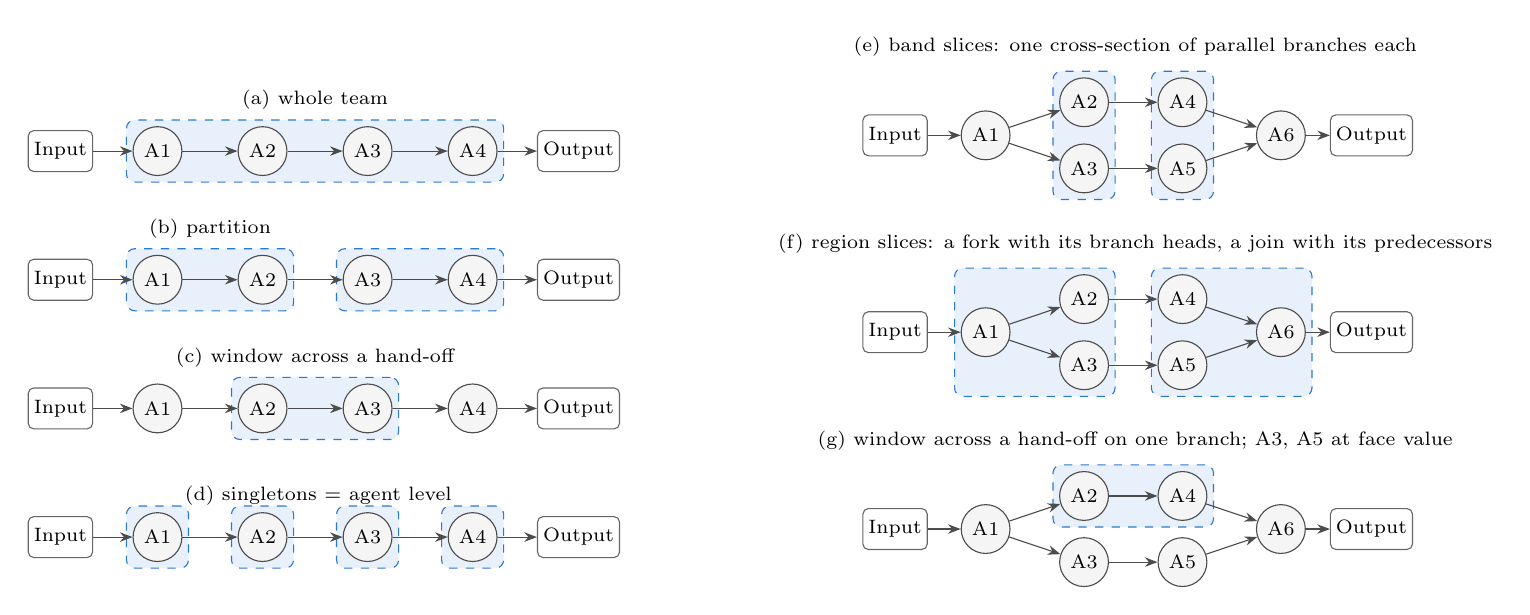
\begin{tikzpicture}[node distance=7mm]
\begin{scope}
\node[io] (i1) {Input};
\node[ag,right=5mm of i1] (a1) {A1};
\node[ag,right=of a1] (a2) {A2};
\node[ag,right=of a2] (a3) {A3};
\node[ag,right=of a3] (a4) {A4};
\node[io,right=5mm of a4] (o1) {Output};
\foreach \u/\v in {i1/a1,a1/a2,a2/a3,a3/a4,a4/o1} \draw[fl] (\u)--(\v);
\begin{scope}[on background layer]
\node[slc,fit=(a1)(a4),label={[font=\scriptsize]above:(a) whole team}] {};
\end{scope}
\node[io,below=11mm of i1] (i2) {Input};
\node[ag,right=5mm of i2] (b1) {A1};
\node[ag,right=of b1] (b2) {A2};
\node[ag,right=of b2] (b3) {A3};
\node[ag,right=of b3] (b4) {A4};
\node[io,right=5mm of b4] (o2) {Output};
\foreach \u/\v in {i2/b1,b1/b2,b2/b3,b3/b4,b4/o2} \draw[fl] (\u)--(\v);
\begin{scope}[on background layer]
\node[slc,fit=(b1)(b2),label={[font=\scriptsize]above:(b) partition}] {};
\node[slc,fit=(b3)(b4)] {};
\end{scope}
\node[io,below=11mm of i2] (i3) {Input};
\node[ag,right=5mm of i3] (c1) {A1};
\node[ag,right=of c1] (c2) {A2};
\node[ag,right=of c2] (c3) {A3};
\node[ag,right=of c3] (c4) {A4};
\node[io,right=5mm of c4] (o3) {Output};
\foreach \u/\v in {i3/c1,c1/c2,c2/c3,c3/c4,c4/o3} \draw[fl] (\u)--(\v);
\begin{scope}[on background layer]
\node[slc,fit=(c2)(c3),label={[font=\scriptsize]above:(c) window across a hand-off}] {};
\end{scope}
\node[io,below=11mm of i3] (i4) {Input};
\node[ag,right=5mm of i4] (d1) {A1};
\node[ag,right=of d1] (d2) {A2};
\node[ag,right=of d2] (d3) {A3};
\node[ag,right=of d3] (d4) {A4};
\node[io,right=5mm of d4] (o4) {Output};
\foreach \u/\v in {i4/d1,d1/d2,d2/d3,d3/d4,d4/o4} \draw[fl] (\u)--(\v);
\begin{scope}[on background layer]
\foreach \x in {d1,d2,d3,d4} \node[slc,fit=(\x)] {};
\node[font=\scriptsize,above=0.5mm of d1.north east,anchor=south west] {(d) singletons = agent level};
\end{scope}
\end{scope}
\def\fjteam#1{%
\node[io] (#1i) at (0,0) {Input};
\node[ag] (#1a1) at (1.15,0) {A1};
\node[ag] (#1a2) at (2.4,0.42) {A2};
\node[ag] (#1a3) at (2.4,-0.42) {A3};
\node[ag] (#1a4) at (3.65,0.42) {A4};
\node[ag] (#1a5) at (3.65,-0.42) {A5};
\node[ag] (#1a6) at (4.9,0) {A6};
\node[io] (#1o) at (6.05,0) {Output};
\foreach \u/\v in {i/a1,a1/a2,a1/a3,a2/a4,a3/a5,a4/a6,a5/a6,a6/o} \draw[fl] (#1\u)--(#1\v);}
\begin{scope}[xshift=10.6cm,yshift=0.2cm]
\fjteam{e}
\begin{scope}[on background layer]
\node[slc,fit=(ea2)(ea3)] {};
\node[slc,fit=(ea4)(ea5)] {};
\end{scope}
\node[font=\scriptsize,anchor=south] at (3.05,0.88) {(e) band slices: one cross-section of parallel branches each};
\end{scope}
\begin{scope}[xshift=10.6cm,yshift=-2.3cm]
\fjteam{f}
\begin{scope}[on background layer]
\node[slc,fit=(fa1)(fa2)(fa3)] {};
\node[slc,fit=(fa4)(fa5)(fa6)] {};
\end{scope}
\node[font=\scriptsize,anchor=south] at (3.05,0.88) {(f) region slices: a fork with its branch heads, a join with its predecessors};
\end{scope}
\begin{scope}[xshift=10.6cm,yshift=-4.8cm]
\fjteam{g}
\begin{scope}[on background layer]
\node[slc,fit=(ga2)(ga4)] {};
\end{scope}
\node[font=\scriptsize,anchor=south] at (3.05,0.88) {(g) window across a hand-off on one branch; A3, A5 at face value};
\end{scope}
\end{tikzpicture}
\end{adjustbox}
\caption{Slices of a chain (a--d, left) and of a team with a fork and a join (e--g, right). Slicing is defined on the team graph, not on a sequence: the same notions apply when agents branch and re-merge. A slice is a convex set of agents analyzed exactly while the rest of the team is taken at face value. Singleton slices (d) give agent-level analysis; the whole team (a) gives exact monolithic analysis. Slices in between expose and localize defects that live in hand-offs, joins and shared models. On the graph, slices may follow a cross-section of parallel branches (e), wrap a fork or a join (f), or follow one branch (g); a slice such as those in (e) need not be connected.}
\label{fig:overview}
\Description{Agent slicing on a chain and on a branching team. Highlighted convex subsets show whole-team, individual-agent, and intermediate analyses.}
\end{figure}

% =====================================================================
\section{Background: Agent Teams and Their Semantics}\label{sec:background}

This section gives the background and formal model needed to define agent slicing. We start with two small software teams that serve as running examples (Section~\ref{sec:running}). We then define teams, with their agents, gates and contracts (Section~\ref{sec:team}), and the runs that resolve a team's routing choices, join policies, and model failures. Next we define the symptoms used to assess safety, and show why these runs suffice to analyze every behavior that respects the contracts. Each definition is followed by a short example on the running teams. Table~\ref{tab:notation} summarizes the notation.

\begin{table}[tbp]
\caption{Notation}
\label{tab:notation}
\centering
\normalsize
\begin{tabularx}{\linewidth}{@{}lY@{}}
\toprule
Symbol & Meaning\\
\midrule
$\Props$ & properties (facts about the work product)\\
$\Phi,\Phi_c$ & goals of the team; critical goals\\
$f$ & fault budget: how many models may fail in one run\\
$N,E,\iota,\omega$ & nodes, edges, input node, output node\\
$\kappa(n)$ & kind of node $n$: agent or gate\\
$\rt(n),\jn(n)$ & routing (fork or switch) and join policy of $n$\\
$\req,\gua,\decl$ & requirements, guarantees, declared evidence of a node\\
$\orc(n)$ & the model (oracle) an agent uses\\
$\rho=(W,C,F)$ & a run: switch choices, contributor sets, failed oracles\\
$c(v),o(v)$ & content (what $v$ receives) and output of $v$ in a run\\
$\key{kind}{v}{p}$ & a symptom key: kind, node, property\\
$\Sym(T)$ & all symptoms of team $T$ (exact semantics)\\
$\sigma$ & a slice (convex node set)\\
$H_\sigma$ & hybrid semantics: $\sigma$ exact, rest at face value\\
$\Fd{\sigma}$ & raw findings of $\sigma$ (keys of $H_\sigma$)\\
$\mathcal{C}(\sigma)$ & confirmed findings of $\sigma$ (witness lifts to $T$)\\
$\depth(\kappa),\MMS(\kappa)$ & depth; minimal confirming slices of key $\kappa$\\
\bottomrule
\end{tabularx}
\end{table}

\subsection{Running Example}\label{sec:running}

We use two small software teams throughout (Fig.~\ref{fig:running}). Each is a pipeline of \emph{agents}, which are driven by language models, and \emph{gates}, which are deterministic programs such as a test runner. A step needs certain facts about the work product before it can start and establishes new facts when it finishes. The next subsections define these notions precisely, and each definition is followed by an example on these two teams.

\begin{figure}[!t]
\centering
\begin{adjustbox}{max width=\linewidth}
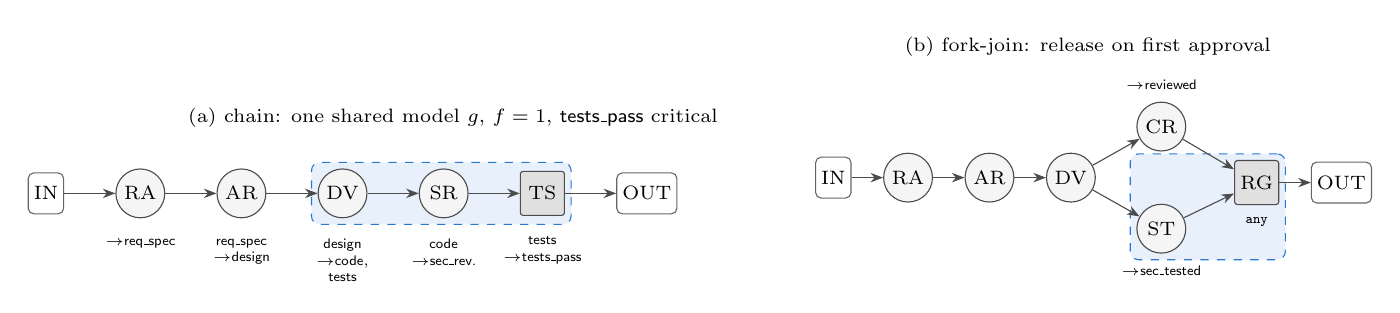
\begin{tikzpicture}[node distance=6.5mm]
\node[io] (in) {IN};
\node[ag,right=of in] (ra) {RA};
\node[ag,right=of ra] (ar) {AR};
\node[ag,right=of ar] (dv) {DV};
\node[ag,right=of dv] (sr) {SR};
\node[gt,right=of sr] (ts) {TS};
\node[io,right=of ts] (out) {OUT};
\foreach \u/\v in {in/ra,ra/ar,ar/dv,dv/sr,sr/ts,ts/out} \draw[fl] (\u)--(\v);
\begin{scope}[font=\tiny,align=center,inner sep=1pt]
\node[below=2.2mm of ra] {$\to$\p{req\_spec}};
\node[below=2.2mm of ar] {\p{req\_spec}\\$\to$\p{design}};
\node[below=2.2mm of dv] {\p{design}\\$\to$\p{code},\\\p{tests}};
\node[below=2.2mm of sr] {\p{code}\\$\to$\p{sec\_rev.}};
\node[below=2.2mm of ts] {\p{tests}\\$\to$\p{tests\_pass}};
\end{scope}
\begin{scope}[on background layer]
\node[slc,fit=(dv)(ts)] {};
\end{scope}
\node[font=\scriptsize,above=4mm of ar,anchor=south west,xshift=-8mm] {(a) chain: one shared model $g$, $f=1$, \p{tests\_pass} critical};
\begin{scope}[xshift=10.0cm,yshift=0.2cm]
\node[io] (in2) {IN};
\node[ag,right=4mm of in2] (ra2) {RA};
\node[ag,right=4mm of ra2] (ar2) {AR};
\node[ag,right=4mm of ar2] (dv2) {DV};
\node[ag,above right=2mm and 7mm of dv2] (cr2) {CR};
\node[ag,below right=2mm and 7mm of dv2] (st2) {ST};
\node[gt,below right=2mm and 7mm of cr2] (rg2) {RG};
\node[io,right=4mm of rg2] (out2) {OUT};
\foreach \u/\v in {in2/ra2,ra2/ar2,ar2/dv2,dv2/cr2,dv2/st2,cr2/rg2,st2/rg2,rg2/out2} \draw[fl] (\u)--(\v);
\node[font=\tiny,below=0.3mm of rg2] {\texttt{any}};
\node[font=\tiny,above=0.3mm of cr2] {$\to$\p{reviewed}};
\node[font=\tiny,below=0.3mm of st2] {$\to$\p{sec\_tested}};
\node[font=\scriptsize,above=11mm of ar2,anchor=south west,xshift=-12mm] {(b) fork-join: release on first approval};
\begin{scope}[on background layer]
\node[slc,fit=(st2)(rg2)] {};
\end{scope}
\end{scope}
\end{tikzpicture}
\end{adjustbox}
\caption{Running example. Circles are agents, squares are gates. Labels show requirements and ($\to$) guarantees. Checking each component alone reports nothing for either team. Shaded: the components whose interaction causes the defect, $\{$DV, SR, TS$\}$ for the chain (a robust loss of \p{tests\_pass}) and $\{$ST, RG$\}$ (one of two) for the fork-join team. Section~\ref{sec:approach} makes this precise.}
\label{fig:running}
\Description{Software-development team with developer, reviewer, test, and release gates. Highlighted slices expose lost approvals and guarantees that depend on a shared model.}
\end{figure}

\textbf{Chain.} A requirements analyst (RA) writes a specification. An architect (AR) turns it into a design. A developer (DV) writes code and tests. A security reviewer (SR) reviews the code. A deterministic test runner (TS) runs the tests and establishes that they pass. The team promises two things: the tests pass (\p{tests\_pass}) and the code is security reviewed (\p{sec\_reviewed}). The first is \emph{critical}: it must hold even if one language model fails ($f=1$). All four agents use the same model $g$.

Look at each component alone. AR needs \p{req\_spec}, which RA guarantees upstream. DV needs \p{design}, guaranteed by AR. SR needs \p{code} and TS needs \p{tests}, both guaranteed by DV. The critical goal is guaranteed by a gate, so it seems not to depend on any model. Every assumption is matched, so an agent-level check, which examines each component against its own contract, reports nothing. Yet the team is not robust. If the shared model $g$ fails, the tests DV writes are not adequate, TS cannot establish \p{tests\_pass}, and the release lacks its critical goal. The defect is neither in DV (it is allowed to fail, since $f=1$) nor in TS (it behaves correctly). It lies in the relationship: \emph{a deterministic gate's critical guarantee rests on a fallible agent's provision.}

\textbf{Fork-join.} The analyst, architect and developer again form a chain. The developer's code then forks to a code reviewer (CR), which guarantees \p{reviewed}, and a security tester (ST), which guarantees \p{sec\_tested}. Both feed a release gate (RG) with policy \texttt{any}: release on the first approval. Every requirement is matched and every goal is claimed by an ancestor of the output, so agent-level analysis is silent. But a run in which RG uses only CR's approval releases code that was not security tested, and the converse run releases code that was not reviewed.

\subsection{Agents, Gates and Contracts}\label{sec:team}

A team works on a shared artifact, for example a code change, and builds up facts about it: a design exists, adequate tests exist, the tests pass. We call such facts \emph{properties} and write $\Props$ for the finite set of properties a team mentions. A component \emph{requires} some properties before it can do its job, and it \emph{guarantees} others when it does its job. This is design by contract~\cite{meyer1992applying} applied to team members.

%Assume-guarantee reasoning connects these component contracts: each component assumes properties of its inputs and guarantees properties of its outputs, and composition requires discharging each assumption~\cite{misra1981proofs,jones1983tentative,abadi1993composing,benveniste2018contracts}. For agent teams, this means checking whether the guarantees actually delivered along the team's possible execution paths establish the requirements of downstream components and the team's goals.

%Properties are semantic claims, not artifacts. ``\p{tests}'' means that an adequate test suite exists, not that a file named \texttt{tests} was produced. When an agent's model fails, the agent may still produce an artifact, for example a weak test suite, but the property it claims does not hold. A downstream test runner that requires \p{tests} then cannot establish \p{tests\_pass}, even if it executes and reports success. So the model covers errors of commission (a wrong artifact presented as right, such as a test suite with vacuous assertions) as well as omission (no artifact at all, such as no tests written), at the level of properties: in both cases \p{tests} does not hold. What the model does not distinguish is what happens next. A symptom at the output says that the team can release without the property being established. It does not say whether the release is a false certification (the runner reports ``pass'' on weak tests) or a visible failure that a later step would catch (the runner reports ``fail'' and someone retries). Safety here is partial correctness: a run that never reaches the output produces no symptom, so a pipeline that blocks on a failed check is safe in the model only if the block is modeled as not reaching the output.

Two kinds of components matter. An \emph{agent} is driven by a language model. Its guarantee is \emph{conditional}: it holds only when the agent's requirements are met and its model (its \emph{oracle}) does not fail. A \emph{gate} is a deterministic program, such as a test runner or a schema check. A gate's guarantee is conditional on its requirements but never on a model.

%An agent may also \emph{declare} evidence for itself, for example ``I read the specification''. Declared evidence counts when we decide whether that agent can act, but it never flows to other components. Semantically, declaring $p$ is the same as removing $p$ from the agent's own requirements. We keep the notion because it records a common documentation practice and makes its locality explicit. For example, if DV declares \p{design} (``I read the design''), DV may act even when no upstream component supplies \p{design}, but TS downstream still does not receive \p{design} from DV.

\begin{definition}[Team]\label{def:team}
A \emph{team} $T$ consists of a graph, node contracts, models, coordination rules, and goals:
\begin{itemize}
\item Graph. A finite directed acyclic graph $(N,E)$ with a unique source $\iota$ (the input) and a unique sink $\omega$ (the output). Every node lies on a path from $\iota$ to $\omega$.
\item Node contracts. Each node $n$ has a kind $\kappa(n)\in\{\mathsf{agent},\mathsf{gate}\}$ and three sets of properties: requirements $\req(n)$, guarantees $\gua(n)$, and declared evidence $\decl(n)$, all subsets of $\Props$. The input $\iota$ and the output $\omega$ are gates, because they run no model. The guarantees $\gua(\iota)$ are the input facts.
\item Models. Each agent $n$ uses an oracle $\orc(n)$. Agents may share an oracle.
\item Coordination. Routing $\rt(n)\in\{\mathsf{fork},\mathsf{switch}\}$ says whether $n$ delivers to all successors or to exactly one. A node with several predecessors has a join policy $\jn(n)\in\{\mathsf{all}\}\cup\{1,\ldots,|\pred(n)|\}$, where a number is a quorum and \textnormal{\texttt{any}} is the quorum $1$.
\item Goals and faults. The goals $\Phi\subseteq\Props$ are required by the output ($\req(\omega)=\Phi$). The critical goals $\Phi_c\subseteq\Phi$ must survive failures, and the fault budget $f\in\mathbb{N}$ bounds how many oracles may fail in one run.
\end{itemize}
Formally, $T=(N,E,\iota,\omega,\kappa,\req,\gua,\decl,\orc,\rt,\jn,\Phi,\Phi_c,f)$.
\end{definition}

We write $\pred(n)$ and $\succs(n)$ for direct predecessors and successors, and $\anc(n)$ and $\desc(n)$ for proper ancestors and descendants. The starred forms $\anc^*$ and $\desc^*$ include the node itself. A switch with one successor is a fork.

\begin{example}[A team]\label{ex:team}
The Chain has seven nodes in a line: the input IN, the agents RA, AR, DV and SR, the gate TS, and the output OUT. The labels in Fig.~\ref{fig:running} give the contracts. For instance, $\req(\p{DV})=\{\p{design}\}$ and $\gua(\p{DV})=\{\p{code},\p{tests}\}$, while the gate TS has $\req(\p{TS})=\{\p{tests}\}$ and $\gua(\p{TS})=\{\p{tests\_pass}\}$. The four agents share one oracle, $\orc(\p{RA})=\orc(\p{AR})=\orc(\p{DV})=\orc(\p{SR})=g$. Every node has one successor and at most one predecessor, so routing and join policies play no role. The goals are $\Phi=\{\p{tests\_pass},\p{sec\_reviewed}\}$ with $\Phi_c=\{\p{tests\_pass}\}$, and $f=1$. The Fork-join team differs in its graph and policies: DV has two successors CR and ST, and the gate RG has two predecessors with join policy \texttt{any}.
\end{example}

\subsection{Runs}

A run fixes every choice the team leaves open and then computes what each node receives and produces. Three kinds of choice remain open: which successor a switch picks, which delivered inputs a quorum or \texttt{any} join actually uses, and which oracles fail.

\begin{definition}[Run]\label{def:run}
A \emph{run} $\rho=(W,C,F)$ consists of
\begin{itemize}
\item a \emph{switch choice} $W(n)\in\succs(n)$ for each switch $n$;
\item a \emph{contributor set} $C(n)$ for each node $n$ with several predecessors, namely the in-edges whose outputs $n$ uses;
\item a set $F$ of \emph{failed oracles} with $|F|\le f$.
\end{itemize}
A run is \emph{fault-free} if $F=\emptyset$. Given $\rho$, process the nodes in topological order. The input $\iota$ is reached, with content $c(\iota)=\emptyset$ and output $o(\iota)=\gua(\iota)$. For every other node $v$:
\begin{enumerate}
\item \emph{Delivery.} An edge $(u,v)$ is \emph{delivered} if $u$ is reached and either $u$ is a fork or $W(u)=v$. Let $D(v)$ be the set of delivered in-edges of $v$.
\item \emph{Reached.} $v$ is reached if $D(v)$ satisfies its join policy: all in-edges for \textsf{all} (and for a node with a single in-edge), at least $q$ in-edges for quorum $q$.
\item \emph{Contributors.} For \textsf{all}, $C(v)$ is all in-edges. For quorum $q$, $C(v)$ is a subset of $D(v)$ with $|C(v)|\ge q$.
\item \emph{Content.} The content of $v$ is the union of the outputs it uses: $c(v)=\bigcup_{(u,v)\in C(v)} o(u)$.
\item \emph{Applies.} $v$ \emph{applies} if $\req(v)\subseteq c(v)\cup\decl(v)$ and either $v$ is a gate or its oracle has not failed ($\orc(v)\notin F$).
\item \emph{Output.} $o(v)=c(v)\cup\gua(v)$ if $v$ applies, and $o(v)=c(v)$ otherwise.
\end{enumerate}
\end{definition}

Properties flow along the contributing lineage. A join that uses one branch forgets what the other branch established. This is what makes \texttt{any} and quorum joins interesting.

\begin{example}[Runs]\label{ex:run}
The Chain has no switches and no joins, so a run is determined by $F$. In the fault-free run $F=\emptyset$, every agent applies. RA outputs \p{req\_spec}, AR adds \p{design}, DV adds \p{code} and \p{tests}, SR adds \p{sec\_reviewed}, and TS adds \p{tests\_pass}. The content of OUT contains both goals. In the run $F=\{g\}$, all four agents use $g$, so none of them applies and none adds a property. TS receives no \p{tests}, cannot apply, and the content of OUT lacks \p{tests\_pass}. In the Fork-join team, the gate RG receives both CR's and ST's outputs but, with policy \texttt{any}, a run may choose $C(\p{RG})=\{(\p{CR},\p{RG})\}$. Then $c(\p{RG})$ contains \p{reviewed} but not \p{sec\_tested}, because the join forgets ST's branch.
\end{example}

\subsection{Symptoms and Safety}

A team can go wrong in three observable ways: a component acts without a property it requires, the output misses a goal, or the output misses a critical goal when up to $f$ oracles fail. We name each by a \emph{key}, a triple of kind, node and property.

\begin{definition}[Symptoms, safety]\label{def:sym}
The \emph{symptoms} $\Sym(T)$ of a team are the keys
\begin{itemize}
\item $\key{assume}{v}{p}$: some fault-free run reaches $v\neq\omega$ with $p\in\req(v)\setminus(c(v)\cup\decl(v))$;
\item $\key{goal}{\omega}{\varphi}$: some fault-free run reaches $\omega$ with $\varphi\in\Phi\setminus c(\omega)$;
\item $\key{robust}{\omega}{\varphi}$: $\key{goal}{\omega}{\varphi}\notin\Sym(T)$, and some run with $|F|\le f$ reaches $\omega$ with $\varphi\in\Phi_c\setminus c(\omega)$.
\end{itemize}
$T$ is \emph{safe} if $\Sym(T)$ contains no goal or robust key, and \emph{clean} if $\Sym(T)=\emptyset$.
\end{definition}

Two remarks on scope. Safety is a partial-correctness notion: a run in which the output is never reached (for example, an \textsf{all}-join behind a switch) produces no symptom. And under failures we check only critical goals at the output, since an agent acting without its requirements because an upstream model failed is the expected consequence of the failure, not a design defect.

\begin{example}[Symptoms]\label{ex:sym}
In the Chain, every fault-free run meets every requirement and delivers both goals, so $\Sym(T)$ has no assume key and no goal key. The run $F=\{g\}$ misses the critical goal \p{tests\_pass} at OUT, so $\Sym(T)$ contains the key $\key{robust}{\p{OUT}}{\p{tests\_pass}}$ and the Chain is not safe. (Under $F=\{g\}$ the downstream agents also act without their requirements, but this is the expected consequence of the failure, not a symptom.) In the Fork-join team, the run in which RG uses only CR misses \p{sec\_tested}, and the converse run misses \p{reviewed}. Its symptoms are therefore $\key{goal}{\p{OUT}}{\p{sec\_tested}}$ and $\key{goal}{\p{OUT}}{\p{reviewed}}$. An assume key would arise, for instance, if AR did not guarantee \p{design}: then $\key{assume}{\p{DV}}{\p{design}}$ would be a symptom.
\end{example}

\subsection{From Models to Runs}

A run assumes that a component knows exactly what it was told: its content, plus any evidence it declared. A real agent may know more. It may happen to hold a fact that nobody guaranteed, for example from its own training. We want conclusions that hold for every behavior that respects the contracts, so we describe such behaviors explicitly and then show that plain runs are enough.

\begin{definition}[Contract-respecting model]\label{def:model}
A \emph{model} of a team $T$ is a run $(W,C,F)$ together with an \emph{evidence set} $E(v)$ for every reached node $v$, where $E(v)\supseteq c(v)\cup\decl(v)$. The set $E(v)$ is everything $v$ knows when it acts: what it was told, what it declared, and possibly more. Two things change compared with Definition~\ref{def:run}.
\begin{itemize}
\item $v$ applies if $\req(v)\subseteq E(v)$ (instead of $\req(v)\subseteq c(v)\cup\decl(v)$) and its oracle has not failed.
\item The keys of Definition~\ref{def:sym} are read with $E(v)$ in place of $c(v)\cup\decl(v)$, and with $E(\omega)$ in place of $c(\omega)$.
\end{itemize}
Contents and outputs are otherwise computed as in a run. A run is the special case $E(v)=c(v)\cup\decl(v)$.
\end{definition}

\begin{example}[A model]\label{ex:model}
Take the Chain with $F=\{g\}$, so DV's model has failed and no \p{tests} reach TS. In the run, TS knows nothing and cannot apply, so \p{tests\_pass} is lost. A model may instead let TS know \p{tests} anyway, with $E(\p{TS})=\{\p{tests}\}$. Then TS applies and establishes \p{tests\_pass}, although no component guaranteed \p{tests}.
\end{example}

Models differ from runs only by this extra evidence. It is a modeling choice: a component may know more than it was told, but never less. Extra evidence can only make components apply, so it can hide a defect but never create one. The run with the least evidence is therefore the worst case, and the following lemmas show that runs, and only a few of them, suffice.

\begin{lemma}[Worst case]\label{lem:w}
A key is produced by some model if and only if it is produced by some run.
\end{lemma}

\begin{lemma}[Minimal choices]\label{lem:m}
Content is monotone in the contributor sets and antitone in the failure set. To decide $\Sym(T)$ it suffices to enumerate runs whose quorum joins use exactly $q$ contributors and whose failure sets have size $\min(f,|\Orc|)$.
\end{lemma}

The idea behind Lemma~\ref{lem:w} is that more evidence can only make more components apply, which only adds properties downstream. The minimal evidence $c(v)\cup\decl(v)$ is the worst case. Proofs are in Appendix~\ref{app:proofs}.

\begin{example}[Using the lemmas]\label{ex:lemmas}
In the example above, the model in which TS knows \p{tests} hides the defect, and the run exposes it (Lemma~\ref{lem:w}). In the Fork-join team, a run in which RG uses both branches contains more than either one-branch run, so it suffices to consider the runs in which RG uses exactly one branch (Lemma~\ref{lem:m}). In the Chain, $\min(f,|\Orc|)=1$, so it suffices to fail $g$.
\end{example}

% =====================================================================
\section{Agent Slicing}\label{sec:approach}

\subsection{Overview}\label{sec:approach-overview}

Agent slicing has three steps (Fig.~\ref{fig:method}). It analyzes groups of components together to find candidate defects, confirms each candidate against the whole team, and shrinks each confirmed defect to the few components involved.

The input is a declared team model $T$ (Section~\ref{sec:background}) and a \emph{slicing strategy}, which proposes a family $\mathcal{S}$ of convex slices. Singleton slices give agent-level analysis. Larger slices can span hand-offs, parallel branches, joins, and shared models. The following subsections define slices, their semantics, and when their results can be combined.

\begin{figure}[H]
\centering
\begin{adjustbox}{max width=\linewidth}
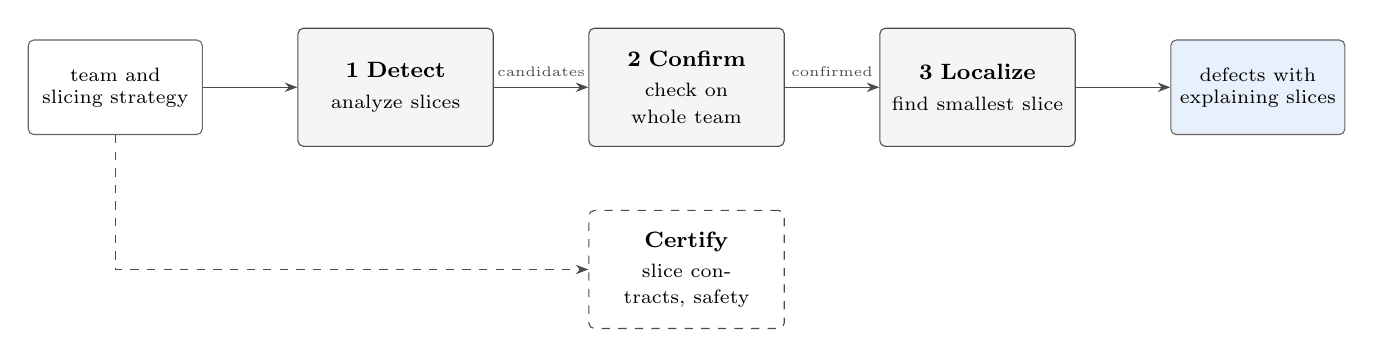
\begin{tikzpicture}[node distance=12mm,
  io/.style={rectangle,rounded corners=2pt,draw=black!60,align=center,font=\scriptsize,text width=2cm,inner sep=3pt,minimum height=1.2cm},
  st/.style={rectangle,rounded corners=2pt,draw=black!70,fill=black!4,align=center,font=\footnotesize,text width=2.2cm,inner sep=4pt,minimum height=1.5cm},
  sd/.style={st,dashed,fill=white},
  lb/.style={font=\tiny,text=black!70,inner sep=1pt}]
\node[io] (in) {team and\\slicing strategy};
\node[st,right=of in] (det) {\textbf{1~Detect}\\[0.5mm]\scriptsize analyze slices};
\node[st,right=of det] (con) {\textbf{2~Confirm}\\[0.5mm]\scriptsize check on whole team};
\node[st,right=of con] (loc) {\textbf{3~Localize}\\[0.5mm]\scriptsize find smallest slice};
\node[io,right=of loc,fill=slicefill] (out) {defects with\\explaining slices};
\draw[fl] (in)--(det);
\draw[fl] (det)--(con) node[lb,midway,above=1mm] {candidates};
\draw[fl] (con)--(loc) node[lb,midway,above=1mm] {confirmed};
\draw[fl] (loc)--(out);
\node[sd,below=8mm of con] (cert) {\textbf{Certify}\\[0.5mm]\scriptsize slice contracts, safety};
\draw[fl,dashed] (in.south) |- (cert.west);
\end{tikzpicture}
\end{adjustbox}
\caption{Overview of agent slicing. Steps 1--3 find, check, and explain defects. Certify (dashed) is separate and decides safety.}
\label{fig:method}
\Description{Pipeline from the team and slicing strategy through three numbered steps, Detect, Confirm and Localize, to defects with explaining slices. A separate dashed Certify box branches from the input.}
\end{figure}

\textbf{Detect.} For each slice $\sigma\in\mathcal{S}$, the checker explores the behavior of the members exactly and takes all other components at face value, meaning it assumes they keep their contracts. It records each symptom it finds together with a \emph{witness}: the choices and failures that expose it. Because the outside is only approximated, some candidates are false alarms.

\textbf{Confirm.} A candidate is reported only after \emph{lifting}. Some run of the whole team must show the symptom, and replaying that run's choices on the slice must show it as well. A confirmed finding is therefore a real defect of the declared team model. Confirming can require a search of the whole team, and a candidate whose search fails or exceeds its budget stays unconfirmed.

\textbf{Localize.} Confirmed findings are merged by symptom key. Each key is localized to its smallest confirming slices among those evaluated, ranked by size and then by number of choice points. The witness shows the mechanism at work: a switch routing around a component that provides the property, a join dropping a contribution, an unmet condition, or an oracle failure. A fixed family of slices can miss a defect or return a larger explanation than necessary. \emph{Shrinking} avoids this. It starts from a whole-team finding, removes a member whenever the remaining slice is still convex and still confirms the key, and repeats. It stops when no single member can be removed, which does not guarantee the smallest possible slice.

\textbf{Summarize and certify.} Slices also have entry assumptions, exit guarantees, and exact boundary behaviors, which describe what a group of components needs and provides. Safety is decided separately, either by exact whole-team checking or by composing boundary behaviors over a partition whose quotient graph is acyclic, using one global failure set (Theorem~\ref{thm:abs}). %Two cautions apply. A flat assumption--guarantee pair may not capture the exact behavior, and finding no confirmed defect in a bounded family of slices does not prove the team safe. Section~\ref{sec:implementation} maps these stages to the code and the reproduction workflow.

\subsection{Slices}

A slice should be a well-defined sub-computation: work that enters it should not leave it and come back. Otherwise the slice's behavior would depend on what happens outside in the middle of its own computation.

\begin{definition}[Slice]\label{def:slice}
A \emph{slice} is a nonempty set $\sigma\subseteq N$ that is \emph{convex}: for all $u,w\in\sigma$, every path from $u$ to $w$ lies in $\sigma$. Its \emph{entry edges} go from outside into $\sigma$, and its \emph{exit edges} go from $\sigma$ to outside. The \emph{hull} $\hull(U)=\anc^*(U)\cap\desc^*(U)$ is the smallest convex superset of $U\subseteq N$.
\end{definition}

Connectedness is not required. In the fork-join team, $\{$CR, ST$\}$ is a slice: there is no path between the two. $\{$RA, DV$\}$ is not a slice, because the path RA$\to$AR$\to$DV leaves it, and its hull is $\{$RA, AR, DV$\}$.

\begin{lemma}[Convexity]\label{lem:convex}
If $\sigma$ is convex, no node outside $\sigma$ is both an ancestor and a descendant of members. Hence outside predecessors of members have no member ancestor. Contracting $\sigma$ to one node (all other nodes kept) leaves a DAG if and only if $\sigma$ is convex.
\end{lemma}

\subsection{Hybrid Semantics}

To analyze a slice in isolation we must say what the rest of the team does. We take it at \emph{face value}: every outside component is assumed to keep its contract and to deliver everywhere.

\begin{definition}[Hybrid semantics]\label{def:hybrid}
For a slice $\sigma$, the \emph{hybrid semantics} $H_\sigma$ computes runs as in Definition~\ref{def:run}, except that members of $\sigma$ are analyzed exactly and all other nodes are taken at face value.
\begin{itemize}
\item \emph{Choices.} A run of $H_\sigma$ fixes only the choices made inside the slice: the switch choices and contributor sets of members, and a failure set $F\subseteq\orc(\sigma)$ with $|F|\le f$.
\item \emph{Outside nodes.} An outside node is reached if it is $\iota$ or if at least one of its in-edges is delivered, whatever its join policy. All its delivered in-edges contribute, it always applies, and it delivers to all its successors.
\item \emph{Entry edges.} Every entry edge into a member $v$ is delivered, and all entry edges carry the same \emph{environment}
\[\env_\sigma(v)=\bigcup_{u\in\pred(v)\setminus\sigma} o(u),\]
the union of the face-value outputs of the outside predecessors of $v$.
\item \emph{Findings.} The \emph{raw findings} $\Fd{\sigma}$ are the keys of Definition~\ref{def:sym} evaluated in $H_\sigma$ at every node. As in Definition~\ref{def:sym}, a robust key is raw only if the goal key of the same property is absent from $\Fd{\sigma}$.
\end{itemize}
Confirmation (Definition~\ref{def:confirmed}) uses a weaker condition on robust keys. A robust key is an \emph{unsuppressed} candidate whenever some run of $H_\sigma$ with failures misses a critical goal at $\omega$, whether or not the slice also shows the goal key.
\end{definition}

By Lemma~\ref{lem:convex}, the outside predecessors of a member are never influenced by members, so $\env_\sigma(v)$ is a fixed set. Outside nodes \emph{below} members are recomputed in each run. This is how an internal failure becomes visible at the output. With $\sigma=N$ nothing is outside, $H_N$ is the exact semantics, and $\Fd{N}=\Sym(T)$. With $\sigma=\emptyset$ every node applies, and $\Fd{\emptyset}$ are the requirements and goals that no ancestor claims at all (\emph{static} keys).

\begin{lemma}[Face value dominates content]\label{lem:face}
Let $\sigma\subseteq\sigma'$, let $\rho'$ be a run of $H_{\sigma'}$, and let $\rho$ be the run of $H_\sigma$ with the same choices on $\sigma$ and failures $F'\cap\orc(\sigma)$. Every node reached in $\rho'$ is reached in $\rho$, and its content in $\rho'$ is a subset of its content in $\rho$.
\end{lemma}

So, run by run, analyzing more components exactly can only remove content. But $H_\sigma$ also has runs with no counterpart in the team. An outside \textsf{all}-join is reached on a single input, and an outside switch delivers to both branches, so $H_\sigma$ over-approximates reachability while it under-approximates missing properties. Its raw findings are therefore neither a may- nor a must-approximation of $\Sym(T)$.

\begin{example}[A raw false alarm]\label{ex:falsealarm}
Let a switch gate $s$ route either to a gate $a$ (which guarantees $x$) or to the output, and let a gate $J$ with an \textsf{all}-join of $\iota$ and $a$ require $x$, and let the output join $s$ and $J$ with \texttt{any}. In the team, $J$ is reached only when $s$ routes to $a$, and then $x$ is present: $\Sym(T)=\emptyset$. In the singleton slice $\{s\}$, $J$ is outside and reached on $\iota$'s edge alone, so $\key{assume}{J}{x}\in\Fd{\{s\}}$.
\end{example}

We therefore never report a raw finding directly.

\begin{definition}[Confirmed findings]\label{def:confirmed}
A raw finding or robust candidate $\kappa$ of $\sigma$ \emph{lifts} if some run $\rho$ of $T$ exhibits $\kappa$ (for a robust key: misses the property at $\omega$ with $1\le|F|\le f$), and the \emph{replay} of $\rho$ on $\sigma$ exhibits $\kappa$ as well. The replay is the run of $H_\sigma$ that makes $\rho$'s switch and contributor choices at members, fails $F\cap\orc(\sigma)$, and, at members that $\rho$ does not reach (but $H_\sigma$ does), uses all delivered inputs and delivers to all successors if a fork and to none if a switch. The \emph{confirmed findings} $\mathcal{C}(\sigma)$ are the keys that lift.
\end{definition}

The definition ties a finding to the slice: the team must show the symptom, \emph{and} the slice must show it for the same internal choices. The implementation first searches team runs with the member switch choices of each recorded witness fixed (up to 64 witnesses per key), and then, if none lifts, searches all runs of the team. Each candidate run is replayed in $H_\sigma$. %The second search is complete. A search that exceeds its budget (e.g., 200{,}000 runs) is counted and the key is treated as unconfirmed, which happened \resConfExhausted{} times in E5. In the worst case, lifting is as hard as whole-team checking (Theorem~\ref{thm:cx}). In our benchmarks a slice finding needed \resSLLifts{} lift searches on average and each took milliseconds.

\subsection{Agent-Level Analysis}

Checking a team agent by agent means examining one component at a time. For each agent $v$, we ask whether $v$ can run into trouble in its own right: whether its requirements are met, whether its model can fail, and, if $v$ is a switch, which branch it takes. Every other component is taken at face value, so it is assumed to keep its contract and to deliver what it promises. This is exactly the hybrid semantics of the singleton slice $\{v\}$ (Definition~\ref{def:hybrid}): $v$ is analyzed exactly, and everything outside $v$ is at face value.

For example, checking DV in the Chain, AR is assumed to deliver \p{design}, so DV's requirement is met. DV's model may fail, but TS is outside the slice and is assumed to keep its contract, so it still delivers \p{tests\_pass}. The check reports nothing. The defect appears only when DV and TS are analyzed together.

\begin{definition}[Agent-level analysis]\label{def:al}
The raw agent-level findings are $\bigcup_{v}\Fd{\{v\}}$, and the (confirmed) agent-level findings are $\AL(T)=\bigcup_{v}\mathcal{C}(\{v\})$.
\end{definition}

\begin{proposition}[What agent level sees]\label{prop:al}
For every node $v$, $\Fd{\emptyset}\subseteq\Fd{\{v\}}$, and the keys located at $v$ in $\Fd{\{v\}}$ are exactly the static keys at $v$. Every key in $\Fd{\{v\}}\setminus\Fd{\emptyset}$ has a witness in which $v$ does not apply (its requirements are unclaimed upstream, or its oracle fails) or $v$ is a switch.
\end{proposition}

The proposition explains the silence in the running example. A singleton slice gives every entry edge the same environment, so a join's own singleton sees the union of its inputs and never the choice it makes. One agent's failure is seen, but never two agents failing together, and a gate never sees where its inputs came from. In the chain, $\Fd{\{v\}}=\emptyset$ for every $v$: the singleton $\{$DV$\}$ can fail, but TS outside still applies at face value.

\subsection{Slice Contracts}

A slice is a component, so it should have a contract. Within a slice, a member's requirement may be established by another member, or it may have to come from outside, and only the latter belong in the slice's assumptions. And the slice guarantees on an exit only what holds there on every behavior.

\begin{definition}[Derived slice contract]\label{def:contract}
For a slice $\sigma$ and an environment $X\subseteq\Props$ carried by every entry edge:
\begin{itemize}
\item the \emph{entry assumptions} $A_\sigma$ are the pairs $(v,p)$ with $v\in\sigma$ and $p\in\req(v)$ such that some fault-free internal run with empty environment reaches $v$ without $p$ in $c(v)\cup\decl(v)$;
\item the \emph{exit guarantee} $G_{\sigma,e}(X)$ of an exit edge $e$ is the intersection, over the fault-free internal runs that deliver $e$, of the output crossing $e$. $G^f_{\sigma,e}(X)$ is the same over runs with $|F|\le f$, and the uniform guarantee is $G_\sigma(X)=\bigcap_e G_{\sigma,e}(X)$;
\item the \emph{naive guarantee} $N_{\sigma,e}(X)$ is what composing member contracts at face value promises on $e$: $X$ plus every guarantee of a member that is an ancestor-or-self of the exit's source.
\end{itemize}
\end{definition}

The gap between naive and derived guarantees is what a slice adds. Each confirmed finding witnesses such a gap, and its witness tells \emph{why} a claimed property did not arrive. For a key $\kappa$ about property $p$ at node $x$, with confirming witness $\rho$ on $\sigma$, each claimer $u$ of $p$ among the ancestors of $x$ is in one of four states: \emph{route} ($u$ is unreached because a switch chose another branch), \emph{drop} ($u$ applied but a join did not take its output into $x$'s lineage), \emph{cond} ($u$ did not apply because a requirement was missing), or \emph{fault} ($u$ did not apply because its oracle failed). The \emph{emergent obligations} $X_\sigma$ are the slice-level conditions that exclude these states, and the taxonomy (Table~\ref{tab:classes}) classifies findings by the state that occurs. Joint coverage excludes \emph{drop}, non-bypass excludes \emph{route}, conditional backing excludes \emph{cond} under failures, and oracle independence excludes two \emph{fault} claimers on one oracle. No single member can carry these obligations: each speaks about two or more components.

Table~\ref{tab:contracts} shows derived contracts for the running example. For $\{$DV, SR, TS$\}$ the fault-free guarantee equals the naive one, but the robust guarantee loses \p{code}, \p{tests}, \p{sec\_reviewed} and \p{tests\_pass}. For $\{$SR, TS$\}$, with \p{tests} supplied from outside, the robust guarantee keeps \p{tests\_pass}, so the slice that \emph{explains} the defect must contain DV. For $\{$ST, RG$\}$ the naive guarantee contains \p{sec\_tested} but the derived one does not: joint coverage fails at RG.

\begin{table}[tbp]
  \caption{Derived and Naive Exit Guarantees in the Running Example (Beyond What the Entries Carry)}
  \label{tab:contracts}
  \centering
  \normalsize
  \begin{tabularx}{\linewidth}{@{}>{\hsize=0.5\hsize}X
                                >{\hsize=1.1667\hsize}X
                                >{\hsize=1.1667\hsize}X
                                >{\hsize=1.1667\hsize}X@{}}
  \toprule
  Slice & Entries carry & Naive $N_\sigma$ & Derived $G_\sigma$ / $G^f_\sigma$\\
  \midrule
  DV, SR, TS & \p{req\_spec}, \p{design} & \p{code}, \p{tests}, \p{sec\_rev.}, \p{tests\_pass} & $G$: same, $G^f$: nothing\\
  SR, TS & $+$\p{code}, \p{tests} & \p{sec\_rev.}, \p{tests\_pass} & $G$: same, $G^f$: \p{tests\_pass}\\
  ST, RG & \p{req\_spec}, \p{design}, \p{code} & \p{sec\_tested} & $G$: nothing\\
  CR, RG & same as above & \p{reviewed} & $G$: nothing\\
  \bottomrule
  \end{tabularx}
  \end{table}

\begin{definition}[Declared contract, exactness]\label{def:declared}
A \emph{declared contract} of $\sigma$ is a pair $(A^d,G^d)$. It is \emph{valid} if, when every entry carries $A^d$, every member's requirements hold in every fault-free internal run and $G^d\subseteq G_{\sigma,e}(A^d)$ for every exit $e$. A pair $(A,G)$ is \emph{exact} for exit $e$ if, for every environment $X$, $G_{\sigma,e}(X)=X\cup G$ when $A\subseteq X$ and $G_{\sigma,e}(X)=X$ otherwise.
\end{definition}

\begin{definition}[Boundary behavior]\label{def:beh}
For a slice $\sigma$ and a failure set $F$, $\Beh_\sigma$ maps each delivery pattern of the entry edges and each assignment of contents to entry edges to the set of possible outcomes: which exits are delivered, with what content, and which keys arise at members. Contents are tracked symbolically: a member's content is the union of the contents of the entry edges in its \emph{flow} plus what members add.
\end{definition}

\begin{theorem}[Slice abstraction]\label{thm:abs}
\begin{enumerate}
\item[(a)] Replacing a convex slice $\sigma$ by a macro component whose behavior is $\Beh_\sigma$ (evaluated with the run's global failure set) leaves every assume and goal key of $T$ unchanged, and leaves the set of properties missing at $\omega$ under each failure set unchanged. Hence $\Sym(T)$ is unchanged.
\item[(b)] Let $f=0$ and let every run of $T$ deliver either all or none of $\sigma$'s entry edges (as for single-entry slices). If $(A^d,G^d)$ is valid and the team in which $\sigma$ is replaced by a component that, when its entries carry $A^d$, delivers on any subset of its exits (possibly none) with content at least $A^d\cup G^d$, and otherwise delivers on any subset with any content, has no goal key, then $T$ has no goal key.
\item[(c)] An exit whose guarantee is $g$ if $r_1$ or $r_2$ enters (two members $r_1\to g$ and $r_2\to g$ feeding one exit node) has no exact single pair $(A,G)$, for any distinct $r_1,r_2,g$.
\item[(d)] Let $\{\sigma_1,\ldots,\sigma_m\}$ partition $N$ (including $\iota$ and $\omega$) into convex parts whose quotient graph is acyclic. Composing the parts' boundary behaviors in the quotient's topological order, with one global failure set per run, yields $\Sym(T)$. Robust keys are decided after composition. Convex parts alone do not suffice: $\{a,d\}$ and $\{b,c\}$ with edges $a\to b$ and $c\to d$ are convex and their quotient has a cycle. With a cyclic quotient, valid flat part contracts can certify an unsafe team.
\end{enumerate}
\end{theorem}

\emph{Proof idea.} (a) and (d) hold because a part's outcomes are a function of what crosses its entries and of the global failure set, and the symbolic flow makes the summary independent of the concrete entry contents. Failure sets must be global because one oracle can serve several parts. This is exactly what makes shared-model defects (S4) visible to composition. Robust keys depend on the absence of a goal key anywhere, so they are decided after composition. (b) follows from (a) because the declared component over-approximates $\Beh_\sigma$ under the stated delivery condition. (c) is the SMT obligation C2 (Table~\ref{tab:proofs}), stated over an uninterpreted sort of properties: exactness on the three environments $\emptyset$, $\{r_1\}$ and $\{r_2\}$ is already contradictory. For the cyclic example add $\iota\to a$, $\iota\to c$, $b\to\omega$, $d\to\omega$ and goals $\{x,y\}$. Let $a$ and $d$ require $y$ and guarantee $x$, and $b$ and $c$ require $x$ and guarantee $y$. The part contracts ``$\{a,d\}$: assume $y$, guarantee $x$'' and ``$\{b,c\}$: assume $x$, guarantee $y$'' are valid and discharge each other, but neither $x$ nor $y$ is ever established and the output misses both goals.

\subsection{Checking Slices and Soundness}

Algorithm~\ref{alg:check} is the slice-level checker. For each slice it enumerates the minimal internal runs (Lemma~\ref{lem:m}) by depth-first search over member choices, propagates each run's effect to outside descendants (stopping where content equals face-value content), collects every distinct witness per key, and confirms keys by lifting. Findings of all slices are merged by key (Proposition~\ref{prop:overlap}), and each key is localized to its inclusion-minimal confirming slices.

\begin{algorithm}[!t]
\caption{Confirmed slice-level checking and localization}\label{alg:check}
\begin{algorithmic}[1]
\REQUIRE team $T$, family of slices $\mathcal{S}$, run budget $B$
\STATE $M \leftarrow$ empty map from keys to (slice, witness) pairs
\FORALL{static keys $\kappa\in\Fd{\emptyset}$}
  \STATE \textbf{if} some run of $T$ reaches $\kappa$'s node \textbf{then} $M[\kappa]\leftarrow\{(\bot,\cdot)\}$
\ENDFOR
\FORALL{$\sigma\in\mathcal{S}$}
  \FORALL{$F\in\{\emptyset\}\cup\{F\subseteq\orc(\sigma):|F|=\min(f,|\orc(\sigma)|)\}$}
    \FORALL{minimal internal run $\rho$ of $\sigma$ with failures $F$ (DFS; abort after $B$)}
       \STATE evaluate members; propagate to outside descendants
       \STATE record each key of $H_\sigma$ with witness $\rho$
    \ENDFOR
  \ENDFOR
  \FORALL{recorded keys $\kappa$ (not static)}
    \STATE \textbf{if} some witness of $\kappa$ lifts (Def.~\ref{def:confirmed}) \textbf{then} add $(\sigma,\rho)$ to $M[\kappa]$
  \ENDFOR
\ENDFOR
\FORALL{keys $\kappa$ in $M$}
  \STATE $\MMS(\kappa)\leftarrow$ inclusion-minimal slices in $M[\kappa]$, ranked by size, then by number of choice points
  \STATE classify $\kappa$ by the claimer states of its witness (Table~\ref{tab:classes})
\ENDFOR
\RETURN $M$, $\MMS$, classes
\end{algorithmic}
\end{algorithm}

\begin{theorem}[Soundness]\label{thm:sound}
\begin{enumerate}
\item[(a)] If the family contains $N$, or if certification composes a partition with an acyclic quotient (Theorem~\ref{thm:abs}d), the verdict ``safe'' implies that $T$ is safe, and each counterexample is a run of $T$.
\item[(b)] Every confirmed finding is a symptom of $T$: $\kappa\in\mathcal{C}(\sigma)$ implies $\kappa\in\Sym(T)$, or, for a robust key, that $T$ loses the property at $\omega$ under at most $f$ failures (and $\Sym(T)$ then contains the robust key or the stronger goal key).
\item[(c)] Raw findings can be false alarms (Example~\ref{ex:falsealarm}).
\end{enumerate}
\end{theorem}

\subsection{A Taxonomy of Blind Spots}

Table~\ref{tab:classes} lists the blind-spot classes. Each is defined by the claimer states in a confirming witness (previous subsection), so the class of a finding is computed, not guessed. The first five classes are visible at agent level. S2--S6 involve a relationship among components, and of these only S5 is visible, at its switch.

\begin{table}[tbp]
\caption{Blind-Spot Classes, Defined by the Claimer States of a Confirming Witness. ``AL'': Visible to Agent-Level Analysis}
\label{tab:classes}
\centering
\normalsize
\begin{tabularx}{\linewidth}{@{}lYp{1.8cm}@{}}
\toprule
Class & Mechanism (witness states) & Agent-level visibility\\
\midrule
A1 & unowned goal: no component claims a goal (static) & yes\\
A2 & missing provider: a requirement no ancestor claims (static) & yes\\
A3 & ordering: the only claimer is not an ancestor of the consumer (static) & yes\\
A4 & single point of failure: the one fallible claimer of a critical goal is in state \emph{fault} & yes\\
S1 & interface gap: provided in a different view (\p{spec@raw} vs.\ \p{spec@summary}) & yes\\
S2 & joint-coverage gap: goal claimers in state \emph{drop} at an \texttt{any}/quorum join & no\\
S3 & path-merge dilution: as S2 for a fact consumed after the join & no\\
S4 & correlated evidence: two or more claimers of a critical goal in state \emph{fault} on one oracle & no\\
S5 & bypass: a claimer in state \emph{route} (a switch routes around it) & at switch\\
S6a & conditional collapse: a gate's critical claim in state \emph{cond} because an agent provision is in state \emph{fault} & no\\
S6b & conditional chain: a goal claimer in state \emph{cond} because a root assumption fails. The root is visible, but the lost goal is not & no\\
\bottomrule
\end{tabularx}
\end{table}

S5 is visible at the switch: the switch's singleton slice explores its choice, so its depth is one. S6b shows that ``visible'' is not ``explained'': agent-level analysis reports the unmet root assumption but never the goal lost several hand-offs later.

\subsection{Depth and Localization}

\begin{definition}[Depth, minimal confirming slices]\label{def:depth}
A slice $\sigma$ \emph{confirms} a key $\kappa$ if $\kappa\in\mathcal{C}(\sigma)$. A confirmed static key has depth $1$ and is localized at its node. Otherwise the \emph{depth} of $\kappa$ is the minimum size of a confirming slice, and $\MMS(\kappa)$ is the set of inclusion-minimal confirming slices. A symptom is \emph{hidden at agent level} if its depth is at least $2$.
\end{definition}

Depth and minimal slices are semantic: they are defined over confirmed findings, so a slice whose face-value world shows a symptom the team does not have, or shows a true symptom for a reason the team does not have, does not count. In the running example, the chain's robust loss of \p{tests\_pass} has depth \resRexChainDepth{} with the unique minimal slice $\{$DV, SR, TS$\}$. SR is included because a slice must be convex. Each goal loss of the fork-join team has depth \resRexFjDepth{} with \resRexFjMinimal{} minimal slices, $\{$CR, RG$\}$ and $\{$ST, RG$\}$: the join together with the branch it may take alone.

\begin{theorem}[Separation]\label{thm:sep}
\begin{enumerate}
\item[(a)] For each class S2, S3, S4, S6a and S6b there is a family of teams, parametric in the number $\ell\ge 0$ of hand-offs between the interacting components (and, for S2 and S3, in the number $m\ge 2$ of branches), in which $\AL(T)$ contains no key of the defect (for S6b: not the goal key), the team is unsafe or unclean, and the defect has depth exactly $2$ (S2, S3) or exactly $\ell+2$ (S4, S6a, S6b).
\item[(b)] Let a \emph{view} of node $v$ be its contract, kind, oracle, policies and the set of properties claimed by its ancestors. Call an analysis \emph{view-disjunctive} if it flags a team if and only if some node's view satisfies a fixed predicate. For S2, S4 and S6a there are safe teams whose views together contain every view of an unsafe team, so no view-disjunctive analysis is both sound and free of false alarms on these classes.
\item[(c)] Recovery: every confirmed agent-level finding is confirmed by every slice that contains its singleton, and every static key at a node $v$ is a raw finding of every slice in which $v$ is reached in some run.
\end{enumerate}
\end{theorem}

Part (b) is a limit on agent-local methods, but only on those that decide one node at a time. An analysis that combines views, such as a check that two claimers share an oracle, escapes it, and so does a global must-analysis, which propagates facts along paths. We compare against both in Section~\ref{sec:eval}. Part (c) follows from the monotonicity of confirmed findings (Theorem~\ref{thm:loc}c). It does not hold for raw findings: a raw agent-level finding can disappear in a larger slice, because the larger slice shows that the singleton's witness was impossible. Together, (a) and (c) make confirmed slice-level analysis strictly more expressive than confirmed agent-level analysis.

\begin{theorem}[Localization]\label{thm:loc}
\begin{enumerate}
\item[(a)] If $\kappa\in\Sym(T)$ then $\MMS(\kappa)\neq\emptyset$. In particular, $N$ confirms $\kappa$.
\item[(b)] $\MMS(\kappa)$ need not be a single slice. It is a single slice if and only if the intersection of the minimal confirming slices is nonempty and confirms $\kappa$.
\item[(c)] Confirmed findings are monotone: if $\sigma\subseteq\sigma'$ are slices, then $\mathcal{C}(\sigma)\subseteq\mathcal{C}(\sigma')$. Hence the confirming slices of a key are closed upward, and $\depth(\kappa)\le k$ iff some slice of size at most $k$ confirms $\kappa$.
\item[(d)] Raw findings are not monotone: there are teams and slices $\sigma\subset\sigma'$ with $\kappa\in\Fd{\sigma}\setminus\Fd{\sigma'}$.
\end{enumerate}
\end{theorem}

For (d), let a switch $s$ route either to a gate $x$ or to the output, let $x$ join $s$ and a provider $y$ of the goal $g$ with \texttt{any}, and let the output join $s$ and $x$ with \textsf{all}. The team is clean. In $\sigma=\{s,x,y\}$ the output is outside and reached on one input. The run in which $s$ routes to $x$ and $x$ uses only $s$'s input misses $g$. In $\sigma\cup\{\omega\}$ that run no longer reaches the output. Larger slices therefore remove raw false alarms as well as reveal deeper defects. Confirmation makes the picture monotone.

\begin{proposition}[Overlap]\label{prop:overlap}
Keys do not depend on the slice that produced them, so findings of overlapping slices merge by key without double counting. A slice only reports the presence of keys, so findings of different slices cannot contradict each other. The family of all convex slices of size at most $k$ confirms every key of depth at most $k$.
\end{proposition}

\subsection{Slicing Strategies}

\begin{definition}[Slicing]\label{def:slicing}
A \emph{slicing} is a family of slices. A \emph{partition slicing} partitions $N$ into slices whose quotient graph is acyclic. A \emph{covering slicing} is any family, and its slices may overlap.
\end{definition}

We compare these strategies. \emph{Singleton} is agent level. \emph{Whole} is the slice $N$. \emph{Window-$k$} takes, for each node, the hull of the node and its descendants within $k-1$ hops. On a chain these are the intervals of length $k$ (Fig.~\ref{fig:overview}c). \emph{Band-$w$} takes the hull of $w$ consecutive longest-path levels, a cross-section of parallel branches (Fig.~\ref{fig:overview}e). \emph{Region} takes single-entry single-exit regions: each fork or switch with its immediate post-dominator, each join with its immediate dominator, and each join with its direct predecessors~\cite{johnson1994program,lengauer1979fast}. \emph{Goal-directed} is the analogue of a backward slice~\cite{weiser1984program}: for each requirement $(v,p)$, the hull of $v$, the ancestors that claim $p$, and the ancestors that claim those claimers' requirements. \emph{Exhaustive-$k$} takes every convex slice of size at most $k$. \emph{SL} is singleton $\cup$ window-2 $\cup$ region $\cup$ goal-directed. \emph{Shrink} starts from the whole team (or a whole-team witness) and greedily removes one member at a time while the slice stays convex and still confirms the key, which yields a slice that is minimal under single removals. The analogy with program slicing is loose: only goal-directed slices have a slicing criterion, and we prove no projection property for them.

\subsection{Complexity}

\begin{theorem}[Complexity]\label{thm:cx}
\begin{enumerate}
\item[(a)] Deciding whether an assume or goal key is in $\Sym(T)$ is NP-complete, already for teams of gates only, without forks, and with $f=0$. Deciding whether a robust key is in $\Sym(T)$ is in $\mathrm{D}^p$ and both NP-hard and coNP-hard. Deciding safety is coNP-complete. Deciding whether a node is reached in some run is NP-complete. Deciding $\depth(\kappa)\le k$ for an assume or goal key is NP-complete.
\item[(b)] Computing $\Fd{\sigma}$ takes $O(R_\sigma\cdot(|N|+|E|)\cdot\lceil|\Props|/w\rceil + R'_\sigma)$ time, where $R_\sigma$ is the number of minimal internal runs, $w$ the machine word size, and $R'_\sigma$ the (quadratic) cost of filtering minimal contributor sets. $R_\sigma$ is bounded by the product of member switch fan-outs, binomial coefficients of member quorum joins, and $1+\binom{|\orc(\sigma)|}{f}$, so it is polynomial when the member choice points and $f$ are bounded. Confirming a finding can cost as much as whole-team checking.
\item[(c)] A team can have $2^{\Theta(|N|)}$ convex slices, and all convex slices of size at most $k$ are enumerated with $O(|N|^k)$ hull tests.
\item[(d)] Singleton, window, band and region strategies produce $O(|N|)$ slices, computable in $O(|N|(|N|+|E|))$ total time, while goal-directed produces at most $\sum_v|\req(v)|$ slices.
\end{enumerate}
\end{theorem}

The hardness of assume and goal keys uses a CNF encoding: one switch per variable chooses a branch that provides $t_i$ or $f_i$, the branches merge with \texttt{any}, and one gate per clause requires the facts that falsify all its literals and guarantees \p{bad}~\cite{cook1971complexity}. The output requires \p{bad}, so a run misses it exactly when the formula is satisfiable. For robust keys, add an agent providing a token after the variable gadgets and make every clause gate require the token and guarantee a critical goal $c$. Failing the agent's oracle always loses $c$, and fault-free runs lose $c$ iff the formula is satisfiable, so the robust key is present iff the formula is unsatisfiable. Hence robust-key membership is not in NP unless NP $=$ coNP. Safety stays coNP-complete because ``some goal or robust key exists'' is equivalent to ``some fault-free run misses a goal or some run with at most $f$ failures misses a critical goal''. Because reachability is NP-hard, Definition~\ref{def:team} requires only that every node lies on an input-output path. A node that no run reaches produces no confirmed finding.

\subsection{Incremental Recertification}

Teams change: a prompt is rewritten, a model is swapped, a join policy is relaxed. Slices make re-verification local.

\begin{theorem}[Incremental recertification]\label{thm:inc}
Let a change modify node $a$, and let $\Delta$ be the symmetric difference of $a$'s old and new guarantees. The dynamic raw findings $\Fd{\sigma}\setminus\Fd{\emptyset}$ of a slice $\sigma$ that is convex in both versions are unchanged unless $\sigma$ intersects $\mathit{Dep}$, where
\begin{itemize}
\item $\mathit{Dep}=\{a\}$ for a change of oracle, kind, routing or join policy;
\item $\mathit{Dep}=\anc^*(a)$ for a change of $\req(a)$ or $\decl(a)$;
\item $\mathit{Dep}=\anc^*(Y)$ with $Y=\{a\}\cup\{y\in\desc(a):\req(y)\cap\Delta\neq\emptyset\}$ for a change of $\gua(a)$.
\end{itemize}
For an edge change $(u,v)$, let $\Delta$ be $u$'s face-value output in either version, and $Y$ be $\{u,v\}$ plus the descendants of $v$ in either version that require a property of $\Delta$. Then $\mathit{Dep}$ is $\anc^*(Y)$ taken in both versions. Static findings are recomputed in linear time. Slices that lose convexity, and slices that a strategy newly generates, are evaluated from scratch. The theorem concerns raw findings. Confirmation depends on the whole team, so stored findings are re-confirmed after each change (one lift search per finding).
\end{theorem}

\emph{Proof idea.} An outside node is taken at face value, so its oracle, kind, routing and policy are invisible to $H_\sigma$. A requirement matters only at its node, which affects $\sigma$'s dynamic findings only if the node is a member or lies below one. A guarantee change alters contents only in the bits of $\Delta$, and those bits matter only at nodes that require them (the output requires the goals).

% =====================================================================
\section{Evaluation}\label{sec:eval}

\subsection{Implementation and Reproducibility}\label{sec:implementation}

The source code and replication package are available in the AgentSlicing GitHub repository~\cite{babaei2026agentslicing}. The replication package implements the approach as a Python library, \texttt{slicing}, with separate modules for the analysis stages outlined in Section~\ref{sec:approach-overview}. Experiments call these modules directly rather than maintaining separate implementations of the proposed checker. The implementation analyzes declared models on CPUs. It neither calls a language model nor requires a GPU. Appendix~\ref{app:grammar} gives the input language and an executable example for a reader's own team.

\subsubsection{From approach components to code}

\textbf{Model representation.} \path{slicing/model.py} defines immutable node records and the \texttt{Team} container, including JSON loading, structural validation, and edits that construct a new team. Construction computes a topological order, predecessor and successor lists, and ancestor and descendant masks. Property names are interned to bit positions, so requirements, guarantees, evidence, and run contents are represented by Python integer bit masks. Slices use a separate node mask. Consequently, union, intersection, membership, and containment checks in the semantics are bitwise operations, while user-facing keys and reports retain node and property names.

\textbf{Candidate generation and hybrid checking.} \path{slicing/slices.py} implements convexity tests, hull closure, exhaustive enumeration, and the singleton, window, band, region, and goal-directed strategies. The analysis accepts the resulting family of node masks, so the strategy can be changed without changing the checker. \path{slicing/semantics.py} caches face-value outputs and static findings for each team and implements \texttt{findings(team, sigma)}. The checker enumerates internal choices using the minimal-contributor and maximal-failure reductions of Lemma~\ref{lem:m}, and records symptom keys with witnesses containing choices and failed oracles. Setting the slice to all nodes gives the exact team semantics through \texttt{symptoms}. Run bounds and deadlines stop expensive searches rather than treating an unfinished search as a safety verdict.

\textbf{Confirmation and localization.} \path{slicing/analysis.py} provides the main entry point, \texttt{check\_confirmed}. It confirms static keys, invokes hybrid checking for each candidate, and calls \texttt{confirm} to search for a lifting run and replay it on the slice. Confirmed keys are collected in a map from a symptom to its confirming slices and witnesses. \texttt{localize} removes non-minimal evaluated slices and ranks the remaining ones, and \texttt{diagnose} assigns the mechanism class from the witness. The returned report contains these findings and statistics on slices, lifting attempts, unconfirmed candidates, run-limit events, exhausted searches, and time-outs. The same module implements the baselines and \texttt{shrink}, which repeatedly removes a node when the remaining slice stays convex and the key remains confirmed. This implementation is greedy: it establishes that no single node can be removed, not that the final slice has globally minimum size.

\textbf{Boundary summaries and recertification.} \path{slicing/contracts.py} implements entry assumptions, per-exit and robust guarantees, declared-contract checks, and the gap from naive composition. \texttt{PartSummary} constructs boundary outcomes lazily and caches them by relevant entry contents, delivery, and failures. \texttt{quotient\_symptoms} composes partition summaries with a global failure set, implementing Theorem~\ref{thm:abs}d. For evolving teams, \path{slicing/incremental.py} computes dependency sets and reuses unaffected \emph{raw} slice findings through \texttt{recertify}. This reuse does not certify previously lifted findings after a change: confirmation still depends on the updated whole team, as stated in Theorem~\ref{thm:inc}.

\subsubsection{Validation and experiment drivers}

Three semantic oracles support conformance testing. The \emph{model oracle}, in \path{slicing/oracle.py}, enumerates contract-respecting models (Definition~\ref{def:model}) with all switch choices, admissible contributor sets, failure sets with $|F|\le f$, and evidence assignments between the realized minimum and that minimum plus the node's requirements and goals. The \emph{replay oracle}, in \path{slicing/conformance.py}, enumerates runs of $H_\sigma$ and replays them with an evaluator that shares no code with the checker's enumerator. The \emph{run oracle} in the same module enumerates runs of $T$ and decides confirmed findings directly from Definition~\ref{def:confirmed}, without the lifting search. These are distinct enumeration procedures, but not completely independent implementations: the replay and run oracles share a replay evaluator with the lifting search's candidate validation. They share no code with the checker's enumerator or the lifting search itself. \path{formal/prove.py} and \path{formal/mutate.py} check the per-node SMT obligations and proof mutants using Z3~\cite{demoura2008z3} version \resZThreeVersion{}. These checks do not mechanize the paper's inductive proofs.

The scripts in \path{experiments/} assemble these components into the evaluations. E1 checks conformance. E2 measures detection and localization on injected defects. E3 analyzes the published-design encodings in \path{experiments/architectures.py}. E4b varies hand-off distance and slice size. E5 measures scalability. E6 checks edits and incremental reuse. E7 measures sensitivity, ablation, and false findings. E8 applies random engineering changes. The topology and contract generator is \path{slicing/generator.py}, the controlled defect injector is \path{slicing/injector.py}, and E8's mutation operators are defined in \path{experiments/e8_mutation.py}. The distinction matters for reproduction: injected classes and depths are controlled inputs in E2, whereas E8 measures the symptoms that result from the selected changes.

%\subsubsection{Reproducing the results}

%Listing~\ref{lst:reproduce} gives the commands from the replication package's root directory. Python~3.12 is the reported environment, and \path{requirements.txt} pins the Python dependencies. The full run is CPU-based and uses process workers according to the available core count. A TeX installation with the ACM class, bibliography style, and packages used by the manuscript is needed only for the PDF build.

%\begin{lstlisting}[float=htbp,language=sh,caption={Reproduction commands, executed from the repository root. The quick and full runs are alternative experiment modes.},label={lst:reproduce}]
% python3 -m venv .venv
% .venv/bin/python -m pip install -r requirements.txt
% make test

% # Quick validation using the bundled remaining results:
% make quick

% # Full regeneration of all experiments and summaries:
% make all

% # Typeset the bundled TOSEM manuscript and preview:
% make -C docs/TOSEM
% \end{lstlisting}

% \texttt{make test} runs the unit and property-based tests. \texttt{make quick} runs the proof obligations, proof mutants, tests, running example, E1, E3, and postprocessing. It does not rerun E2, E4b, or E5--E8. Thus its postprocessed summaries also use the bundled result files for the omitted experiments. For a complete reproduction, use \texttt{make all}, which invokes \path{experiments/run_all.py} and runs every experiment before postprocessing. The driver runs each stage as a separate process, writes its output to \path{results/logs/}, and stops at the first failed stage. A selected stage can also be rerun by name, for example \texttt{.venv/bin/python experiments/run\_all.py e8\_mutation process}. Postprocessing then combines the new E8 file with the other available results. Experiment runs replace their result files, so comparisons with the bundled snapshot should use a separate checkout or a preserved copy.

% \textbf{From executions to reported numbers.} Experiment scripts save raw measurements and findings as \path{results/*.json}. Shared utilities record the commit identifier, working-tree status, Python and numerical-library versions, platform, available CPUs, start time, and elapsed time. Generator and experiment seeds and search budgets are fixed in the scripts. Statistical resampling uses NumPy seed 20261104. \path{scripts/process_results.py} reads the JSON files, computes the statistics and confidence intervals, and writes \path{results/macros.json}, LaTeX result macros, table bodies, and figures. The same script generates the opening figure (Fig.~\ref{fig:teaser}) from the E8 file. Its current output directory is \path{docs/TSE}, and it also replaces the marked generated-results block in that directory's \texttt{main.tex}. The TOSEM source bundles the corresponding numerical snapshot with revised presentation, including merged result tables. Consequently, \texttt{make -C docs/TOSEM} typesets that snapshot. It does not execute experiments or automatically import fresh postprocessor output. A reader can compare a fresh run's generated macros and table bodies with the TOSEM values, and inspect the raw JSON and stage logs when a number differs.

% Reproduction should compare semantic findings, class counts, and statistical summaries together with their recorded seeds and budgets, rather than require byte-identical files: provenance and timings necessarily change. Hardware and load can also change which runs finish within a wall-time budget, affecting censored timings and budget-limited detection coverage. Such differences must be interpreted with the recorded time-out and exhaustion indicators. The supplied JSON files allow the reported snapshot to be audited and its statistics recomputed without rerunning the expensive scalability experiment. This is distinct from independently regenerating the experimental data.

\subsection{Experimental Setup}\label{sec:setup}

An experiment plan with hypotheses, metrics, tests and decision rules was written before the first experiment and is in the replication package, with a deviation log. The plan was not registered with an external service, so its timing cannot be verified independently. Later changes to the method (confirmation), added baselines and benchmarks, and replaced analyses are logged and summarized in Section~\ref{sec:threats}.

Table~\ref{tab:hyp} lists the outcome of each planned hypothesis. E4b and E8 were added after the original plan and are exploratory.

\begin{table}[tbp]
\caption{Planned Hypotheses and Their Outcome}
\label{tab:hyp}
\centering
\normalsize
\begin{tabularx}{\linewidth}{@{}lYY@{}}
\toprule
Hypothesis & Statement & Outcome\\
\midrule
H1.1 & The SMT obligations have their expected validity or countermodel outcomes, and proof mutants are rejected. & Supported.\\
H1.2 & The implementation agrees with brute-force semantic oracles. & Supported on the small teams checked.\\
H2.1 & Slice-level analysis detects relational defects missed by agent-level analysis. & Holds by construction for the injected hidden classes (Theorem~\ref{thm:sep}a); reported as counts.\\
H2.2 & Slicing localizes defects exactly more often than the whole-team and random-slice baselines. & Supported against random slices and the whole-team witness deviation set; not against whole-team detection followed by shrinking.\\
H2.3 & At most 5\% of clean or decoy teams raise a false alarm. & Supported: no alarms on these benchmarks.\\
H3.1 & Slicing strategies have polynomial empirical scaling, whereas whole-team checking does not. & Not supported: behavior depends on topology and choice points.\\
H3.2 & Recall saturates as the maximum slice size $k$ increases. & Follows from the injected gadget sizes; E4b varies hand-off distance and host size.\\
H3.3 & Incremental recertification re-verifies fewer than half of the slices. & Supported in aggregate on non-chain topologies; wall-time savings are small.\\
\bottomrule
\end{tabularx}
\end{table}

\textbf{Benchmarks.} We use three.
\emph{(i) Mutation benchmark (E8).} The generator builds clean teams in seven topologies: chain, tree, fork-join, layered DAG, series-parallel, random DAG, and \emph{mixed} (series-parallel with switches and \texttt{any}-joins). It assigns contracts in topological order, drawing each requirement from a sound lower bound on the node's content, so teams are clean by construction (the exact semantics confirms this). One goal is critical and $f=1$. Each team then receives one to three random engineering changes (retried until that many apply): relax a join from \textsf{all} to a quorum, let two agents share a model, drop a guarantee, turn a gate into an agent, add a requirement, turn a fork into a switch, or remove an edge. Whatever symptoms result are the ground truth, computed with the exact semantics and cross-checked with the replay oracle on teams of up to 12 nodes. Neither the class nor the depth of a defect is chosen by us. We build \resMutTeams{} teams (7 topologies, inner sizes of 6, 10, 20 and 30 nodes, 20 seeds, and 1--3 changes). Symptoms deeper than the enumeration bound (\resMutDeepKeys{} keys) count as hidden, but their localization is not scored.
\emph{(ii) Injected benchmark (E2).} The injector adds exactly one defect of a chosen class to a clean team, as a small gadget with fresh property names, and records the class, the root-cause nodes and the symptom keys (verified with the exact semantics). It also builds \emph{clean} teams and four \emph{decoys}: structures that look suspicious but are safe (an \texttt{any}-join whose branches claim all goals, shared-model reviewers backed by a gate, a switch whose both branches provide the fact, and a fallible provider backed by an independent gate). For each of 7 topologies, 2 host sizes, 10 seeds and 16 classes we build one team, in a \emph{small} benchmark (\resBenchNodesSmallMin--\resBenchNodesSmallMax{} nodes) and a \emph{medium} one (\resBenchNodesMediumMin--\resBenchNodesMediumMax{} nodes). Because each gadget is fixed per class and cannot interact with its host, this benchmark tests per-class behavior. Its class mix, not nature, decides prevalence, so we report no prevalence from it.
\emph{(iii) Published designs (E3)}, encoded with a written protocol (Section~\ref{sec:rq2}).

\textbf{Ground truth for depth and localization.} On teams of at most 16 nodes we enumerate every convex slice of size at most 6, otherwise at most 5, and compute confirmed findings. The inclusion-minimal confirming slices of a key are its true minimal slices. This uses the same hybrid semantics as the checkers, but confirmation is checked against the independent run oracle (Section~\ref{sec:rq1}).

\textbf{Checkers.} \emph{B1} is agent-level analysis (confirmed singleton slices), and \emph{B1-raw} omits confirmation. \emph{SL} and the single strategies are confirmed slice families, and \emph{SL-raw} omits confirmation. \emph{B2} is the exact whole-team checker, which returns a verdict and one witness per key. We localize its findings in three ways: the hull of the witness's contributing lineage (which always contains the input and is therefore the symptom node's whole ancestor cone), the \emph{deviation set} of the witness (failed agents, agents that did not apply, switches, and quorum joins that used fewer inputs than they received, together with the symptom node), which needs no slices, and \emph{B2+shrink}, which shrinks the whole team slice by slice (Section~\ref{sec:approach}). \emph{B3} draws random convex slices matched to SL in number and size. \emph{B4} is a structural lint (coverage by set difference over all claims, ignoring paths). \emph{B5} is a pattern-based smell detector that flags the shapes of S2--S6 without semantics. \emph{B6} is a global must-analysis: a Kildall-style lower bound on content with union at \textsf{all}-joins and intersection at \texttt{any}/quorum joins, run once without failures and once per failure set of size $\min(f,|\Orc|)$, which reports a key wherever the lower bound lacks a required property. It is path-insensitive and linear per failure set, and it localizes to the symptom node.

\textbf{Metrics.} A checker \emph{detects} a key if it reports it. On the injected benchmark the pre-registered metric is ``reports any ground-truth key'', and we also report the defect's primary key (for S6b the lost goal rather than the unmet root assumption), which is what separates the classes. A reported key is \emph{false} if it is not a symptom (a robust key also counts as correct when the team loses the property without failures). Localization uses the top-ranked slice of a key: it is \emph{exact} if it is one of the true inclusion-minimal confirming slices, \emph{minimum} if its size equals the depth, and \emph{precise} if it lies within the hull of the injected root cause. The \emph{size ratio} is its size over $|N|$, and \emph{cost} counts slice checks.

\textbf{Statistics.} Where outcomes are deterministic per class (0\% or 100\% on every seed), we report exact counts and one-sided 95\% Clopper--Pearson bounds instead of tests. For localization we compare per-unit exact rates (unit: topology $\times$ seed) with one-sided Wilcoxon signed-rank tests~\cite{wilcoxon1945individual}, Holm correction~\cite{holm1979simple} and Vargha--Delaney $\hat A_{12}$~\cite{vargha2000critique}, and give 95\% cluster-bootstrap intervals~\cite{efron1993introduction} that resample hosts (topology, size, seed), because each host is reused across classes and checkers~\cite{arcuri2011practical}.

\textbf{Environment.} All experiments run on one machine (20 CPU cores, Linux, Python 3.12, NumPy, SciPy, Z3), with seeds fixed in the scripts. Each result file records the commit, library versions and wall time. One command regenerates all results, tables, figures and every number in this paper.

\subsection{RQ1: Formal Foundation and Expressiveness}\label{sec:rq1}

\textbf{Method.} We validate the theory in three ways. (i) SMT obligations. The per-node steps of the proofs are formulas over arrays from an uninterpreted sort of properties to Booleans, so each holds for every property universe and every contract. An obligation is valid if its negation is unsatisfiable. These are one-step set identities. They guard the definitions against slips, not the inductions over topological order, which are proved on paper. Six \emph{proof mutants} each change one definition (for example, letting declared evidence flow on) and must break the obligation that depends on it. (ii) Conformance. On \resWildTeams{} random ``wild'' teams with arbitrary contracts, policies, switches and faults (3--7 inner nodes) and on \resBenchTeams{} small injected teams (4--7 inner nodes before injection), we compare the implementation with the three oracles and check each computational theorem statement directly, for all convex slices of size at most 3 (2 for the run oracle). (iii) The hardness reductions of Theorem~\ref{thm:cx} on \resReductionFormulas{} random 3-CNF formulas, and the view-disjunctive constructions of Theorem~\ref{thm:sep}b.

\begin{table}[H]
\caption{SMT Proof Obligations (Z3 \resZThreeVersion). ``Valid'': the Negation Is Unsatisfiable, ``Countermodel'': a Satisfying Model Exists, as Intended}
\label{tab:proofs}
\centering
\normalsize
\begin{tabularx}{\linewidth}{@{}lYp{0.20\linewidth}ll@{}}
\toprule
ID & Obligation & Used in & Kind & OK\\
\midrule
\tabProofs
\bottomrule
\end{tabularx}
\end{table}

\begin{table}[H]
\caption{Conformance Against Brute-Force Oracles: Teams Checked (Wild, Injected) and Teams With Any Mismatch}
\label{tab:conformance}
\centering
\normalsize
\begin{tabularx}{\linewidth}{@{}Yrrr@{}}
\toprule
Check & Wild & Inj. & Mism.\\
\midrule
\tabConformance
\bottomrule
\end{tabularx}
\end{table}

\textbf{Results.} All \resProofObligations{} obligations behave as expected (\resProofSteps{} valid steps and \resProofCountermodels{} intended countermodel; Table~\ref{tab:proofs}). The countermodel shows that the conditional transfer does not distribute over intersection, which is why a must-analysis cannot be exact. All \resMutantsKilled{} of \resMutants{} mutants are killed. Table~\ref{tab:conformance} shows \resConformanceMismatches{} mismatching teams in \resConformanceComparisons{} team-check pairs, including confirmed findings against the run oracle, the monotonicity of confirmed findings, partition composition, and incremental recertification after node and edge changes. The model oracle agrees with the run semantics on \resModelOracleTeams{} teams. The reductions agree with a SAT solver on all formulas (\resReductionDisagreements{} disagreements for goal keys, \resReductionRobustDisagreements{} for robust keys, which are present exactly when the formula is unsatisfiable), and the view-disjunctive constructions behave as Theorem~\ref{thm:sep}b states (\resFoolingAllHold{} conditions hold). These checks cover small teams only. They are evidence, not proof, for larger teams.

Conformance testing found two real bugs, both logged in the replication package. A switch with one successor was treated as choosing nothing. Every evaluator read the same field the same way, so the oracles agreed with the checker until a theorem check exposed it. And the first version of lifting fixed the witness's contributor sets, which missed liftable witnesses that differ only in which entry edge or which non-minimal contributor set they use. The run oracle exposed it. Oracles that share a data model can share a misreading of it, and we return to this in Section~\ref{sec:threats}.

\answer{RQ1}{Yes, with qualifications. A slice is a convex set of agents with a hybrid semantics, per-exit derived contracts, and emergent obligations defined over witnesses. Raw slice findings approximate in both directions, but confirmed findings are sound (Theorem~\ref{thm:sound}b) and monotone in the slice (Theorem~\ref{thm:loc}c). The singleton slicing is agent-level analysis, and larger slices recover every confirmed agent-level finding and reveal defect families that it misses (Theorem~\ref{thm:sep}a,c), so confirmed slice-level analysis is strictly more expressive. Analyses that judge one agent's view at a time cannot separate safe from unsafe teams on S2, S4 and S6a (Theorem~\ref{thm:sep}b), but analyses that combine views, such as a global must-analysis, are not covered. Slice abstraction is compositional over partitions with an acyclic quotient and a global failure set (Theorem~\ref{thm:abs}d), and exact slice contracts are not single set-valued assumption-guarantee pairs (Theorem~\ref{thm:abs}c). Confirmation needs a whole-team search, so confirmed analysis is not local (Theorem~\ref{thm:cx}b). Per-node steps are SMT-checked, and the inductions are proved on paper, some steps in sketch form. The \resConformanceComparisons{} oracle comparisons on small teams show no mismatch.}

\subsection{RQ2: Detection and Localization Power}\label{sec:rq2}

\subsubsection{Defects from engineering changes (E8)}

Of the \resMutTeams{} mutated teams, \resMutUnclean{} have at least one symptom and \resMutUnsafe{} are unsafe. Together they have \resMutKeys{} symptom keys. The replay oracle agrees with the exact semantics on all \resMutOracleTeams{} teams it checked (\resMutOracleDisagree{} disagreements).

\textbf{How often are defects hidden?} Most symptoms are visible to an agent-by-agent check: \resMutDepthOne{} keys have depth~1. But \resMutHiddenKeys{} keys (\resMutHiddenShare) have depth at least two: \resMutDepthTwo{} of depth 2, \resMutDepthThree{} of depth 3, \resMutDepthFour{} of depth 4, \resMutDepthFive{} of depth 5 and \resMutDepthSix{} of depth 6. \resMutDeepKeys{} of the hidden keys are deeper than the enumeration bound. \resMutTeamsWithHidden{} teams have at least one hidden key, and in \resMutALDeclaredClean{} of the \resMutUnclean{} defective teams (\resMutALDeclaredCleanUnsafe{} of them unsafe) the confirmed agent-level check reports nothing, so it would declare the team clean. The hidden share depends on team size: \resMutHiddenShareNSix{} at 8 nodes, \resMutHiddenShareNOneZero{} at 12, \resMutHiddenShareNTwoZero{} at 22 and \resMutHiddenShareNThreeZero{} at 32. Agent-level recall on hidden keys is \resMutRecallHiddenBOne{} at every size, and the false rate of the must-analysis B6 stays low, from \resMutBSixFalseRateNSix{} at 8 nodes to \resMutBSixFalseRateNThreeZero{} at 32. The per-size breakdown, with confidence intervals for the localization rates, is in \path{results/e8_mutation.json} of the replication package.

\textbf{Which changes create hidden defects?} Table~\ref{tab:mutop} breaks the results down by change operator. A team can receive up to three changes, so the left block counts every team that contains the operator, and the right block counts only the \resMutSingleChangeTeams{} teams whose single change is that operator, which attributes symptoms more cleanly. Relaxing an \textsf{all}-join is the most dangerous change. \resMutOpRelaxJoinHidden{} of the keys in teams containing it are hidden, and in \resMutOpRelaxJoinALSilent{} of its \resMutOpRelaxJoinUnclean{} defective teams the agent-level check reports nothing. Alone, it creates symptoms in \resMutOpRelaxJoinSingleUnclean{} of \resMutOpRelaxJoinSingleTeams{} teams, and \resMutOpRelaxJoinSingleHidden{} of their keys are hidden. Letting two agents share a model (\resMutOpShareOracleHidden{} hidden) and turning a gate into an agent (\resMutOpGateToAgentHidden{}) come next. Their symptoms are mostly visible when they are the only change (\resMutOpShareOracleSingleHidden{} and \resMutOpGateToAgentSingleHidden{} hidden), so most of their hidden defects arise in combination with other changes. Turning a fork into a switch never creates a symptom alone (\resMutOpForkToSwitchSingleUnclean{} of \resMutOpForkToSwitchSingleTeams{} teams), yet it appears in \resMutOpForkToSwitchUnclean{} defective teams when combined with other changes. Adding a requirement, dropping a guarantee, and removing an edge produce mostly visible defects.

Fig.~\ref{fig:depthbyop} shows how deep these defects are and how the picture changes when changes combine. Alone, relaxing a join is the only change whose symptoms are mostly hidden, and most of them have depth~2: the join together with the branch it may take alone. In teams with two or three changes, every operator takes part in hidden symptoms, from \resMutOpRemoveEdgeComboHidden{} of the keys for removing an edge to \resMutOpRelaxJoinComboHidden{} for relaxing a join, with sharing a model second (\resMutOpShareOracleComboHidden). Sharing a model rises from \resMutOpShareOracleSingleHidden{} hidden alone to \resMutOpShareOracleComboHidden{} in combination, and turning a gate into an agent from \resMutOpGateToAgentSingleHidden{} to \resMutOpGateToAgentComboHidden. This is consistent with the mechanisms of Table~\ref{tab:classes}: correlated evidence (S4) needs two claimers on one model, and a conditional collapse (S6a) needs a gate whose input comes from a fallible agent, so a single change often supplies only one of the two ingredients. Symptoms of depth~3 or more are a minority under every operator. A review that checks each modified agent on its own therefore misses many of the defects that arise when independent changes interact.

\begin{figure}[tbp]
\centering
\begin{adjustbox}{max width=\linewidth}
\figDepthByOp
\end{adjustbox}
\caption{Depth of the symptom keys produced by each change operator in the mutation benchmark (E8): (a) teams whose only change is the operator; (b) teams that combine it with one or two other changes. Depth~1 (gray) is visible to agent-level analysis, and depths of 2 or more (blue) are hidden. $n$: symptom keys. Keys deeper than the enumeration bound are counted in depth~$\ge$4. Operators are ordered by the hidden share in (b).}
\label{fig:depthbyop}
\Description{Two panels of horizontal 100 percent stacked bars, one bar per change operator, split into depth 1, 2, 3 and at least 4. Alone, only relaxing a join produces mostly hidden symptoms, nearly all of depth 2. Combined with other changes, every operator produces hidden symptoms, between about a quarter and two thirds of its keys, with sharing a model and relaxing a join highest.}
\end{figure}

\begin{table}[tbp]
\caption{Mutation Benchmark by Change Operator. Teams: Teams Containing the Operator. Unclean: Those With at Least One Symptom (\%). Keys: Their Symptom Keys. Hidden: Share of Those Keys That Are Hidden (\%). AL Silent: Defective Teams Where the Confirmed Agent-Level Check Reports Nothing. Right Block: Only Teams Whose Single Change Is the Operator}
\label{tab:mutop}
\centering
\normalsize
\setlength{\tabcolsep}{4pt}
\begin{adjustbox}{max width=\linewidth}
\begin{tabular}{@{}lrrrrr@{\hspace{12pt}}rrr@{}}
\toprule
 & \multicolumn{5}{c}{All teams containing the operator} & \multicolumn{3}{c}{Single-change teams}\\
\cmidrule(lr){2-6}\cmidrule(l){7-9}
Operator & Teams & Unclean (\%) & Keys & Hidden (\%) & AL silent & Teams & Unclean (\%) & Hidden (\%)\\
\midrule
\tabMutationByOp
\bottomrule
\end{tabular}
\end{adjustbox}
\end{table}

\begin{table}[tbp]
\caption{Mutation Benchmark: Detection (\% of All and of Hidden Keys), False Findings, and Exact Localization of Hidden Keys}
\label{tab:mutation}
\centering
\normalsize
\setlength{\tabcolsep}{4pt}
\begin{tabularx}{\linewidth}{@{}Yrrrr@{}}
\toprule
Checker & All & Hidden & False/reported & Exact loc.\\
\midrule
\tabMutation
\bottomrule
\end{tabularx}
\end{table}

\textbf{Detection and false findings.} Table~\ref{tab:mutation} compares the checkers. Confirmed agent-level analysis (B1) finds \resMutRecallBOne{} of all keys and \resMutRecallHiddenBOne{} of the hidden ones. Confirmed SL finds \resMutRecallSL{} of all keys and \resMutRecallHiddenSL{} of the hidden ones with no false finding (\resMutFalseSL{} false keys). The few it misses are deeper than any of its slices. Without confirmation, SL would report \resMutFalseSLraw{} false keys (\resMutFalseRateSLraw{} of its findings), and agent-level analysis \resMutFalseRateBOneraw. The global must-analysis B6 is a strong detector: it finds \resMutRecallBSix{} of all keys and \resMutRecallHiddenBSix{} of the hidden ones in linear time per failure set, but \resMutFalseBSix{} of its \resMutReportedBSix{} findings (\resMutFalseRateBSix) are false, because a lower bound on content does not know which nodes are reachable together. The smell detector B5 flags \resMutRecallHiddenBFive{} of the hidden keys but \resMutFalseRateBFive{} of its findings are false, and the lint B4 finds no hidden key.

\textbf{Localization.} For hidden keys, B6 names only the symptom node, which is never a minimal confirming slice of a hidden key. SL's top slice is an exact minimal slice in \resMutExactSL{} of cases, falling from \resMutExactSLNSix{} at 8 nodes to \resMutExactSLNThreeZero{} at 32 nodes: on larger teams its fixed strategies more often return a confirming slice that is not minimal. Shrinking a whole-team witness slice by slice is exact in \resMutShrinkExact{} of cases and minimum-size in \resMutShrinkMinimum, at about \resMutShrinkChecks{} slice checks per key (median \resMutTimeShrink~ms), and it is at least \resMutShrinkExactNThreeZero{} at every size. Combined with the must-analysis as detector, the pipeline detect--confirm--shrink is exact for \resMutPipeExact{} of the hidden keys it detects. Median times per team are \resMutTimeBSix~ms for B6, \resMutTimeBTwo~ms for the exact whole-team check, and \resMutTimeSL~ms for confirmed SL. The deviation set of the whole-team witness, which needs no slices, is exact in only \resMutDevExact{} of cases and covers \resMutDevRatio{} of the team on average: it names every agent that deviated in the run, including those whose deviation does not matter for the symptom.

\subsubsection{Injected defects by class (E2)}

\begin{table}[tbp]
\caption{Injected Benchmark: Recall (\%) of the Primary Injected Symptom by Class and Checker (Small and Medium). Depth From Exhaustive Confirmed Enumeration (Small)}
\label{tab:recall}
\centering
\normalsize
\setlength{\tabcolsep}{2pt}
\begin{tabular*}{\linewidth}{@{\extracolsep{\fill}}llrrrrrrrrrrr@{}}
\toprule
Class & Depth & B1 & SL & Win-2 & Band-1 & Region & Goal & B2 & B3 & B4 & B5 & B6\\
\midrule
A1 & 1 & 100.0 & 100.0 & 100.0 & 100.0 & 100.0 & 100.0 & 100.0 & 100.0 & 100.0 & 0.0 & 100.0\\
A2 & 1 & 100.0 & 100.0 & 100.0 & 100.0 & 100.0 & 100.0 & 100.0 & 100.0 & 100.0 & 0.0 & 100.0\\
A3 & 1 & 100.0 & 100.0 & 100.0 & 100.0 & 100.0 & 100.0 & 100.0 & 100.0 & 0.0 & 0.0 & 100.0\\
S1 & 1 & 100.0 & 100.0 & 100.0 & 100.0 & 100.0 & 100.0 & 100.0 & 100.0 & 100.0 & 0.0 & 100.0\\
A4 & 1 & 100.0 & 100.0 & 100.0 & 100.0 & 0.0 & 100.0 & 100.0 & 100.0 & 100.0 & 0.0 & 100.0\\
S5 & 1 & 100.0 & 100.0 & 100.0 & 100.0 & 100.0 & 100.0 & 100.0 & 100.0 & 0.0 & 100.0 & 100.0\\
S2 & 2 & 0.0 & 100.0 & 100.0 & 0.0 & 100.0 & 100.0 & 100.0 & 99.6 & 0.0 & 100.0 & 100.0\\
S3 & 2 & 0.0 & 100.0 & 100.0 & 0.0 & 100.0 & 100.0 & 100.0 & 100.0 & 0.0 & 100.0 & 100.0\\
S4 & 2--4 & 0.0 & 100.0 & 34.6 & 0.0 & 0.0 & 100.0 & 100.0 & 98.2 & 0.0 & 100.0 & 100.0\\
S6a & 2--4 & 0.0 & 100.0 & 28.2 & 0.0 & 0.0 & 100.0 & 100.0 & 96.1 & 0.0 & 100.0 & 100.0\\
S6b & 2--4 & 0.0 & 100.0 & 34.6 & 0.0 & 0.0 & 100.0 & 100.0 & 98.9 & 0.0 & 0.0 & 100.0\\
\bottomrule
\end{tabular*}
\par\smallskip\raggedright
Win-2: window-2; Goal: goal-directed.
\end{table}

Table~\ref{tab:recall} gives recall of the primary key by class on the \resBenchTotal{} injected teams. The six agent-level classes have depth one and are found by B1. Every injected S2, S3, S4, S6a and S6b defect has depth at least two. B1 finds none of their primary keys (\resRecallHiddenNsingleton{} of \resHiddenTeams), and SL finds all of them (\resRecallHiddenNSL). This contrast is a consequence of Theorem~\ref{thm:sep}a, which the gadgets instantiate, not an independent finding. The experiment confirms that theory and implementation agree across all seven topologies. Under the pre-registered metric (any ground-truth key), B1 detects \resRecallPlanHiddensingleton{} of the hidden-class teams: it reports the unmet root assumption of every S6b team (\resRecallPlanSSixbsingleton), but never the goal that is lost. The must-analysis B6 also finds every primary key here, and raises no alarm on clean or decoy teams.

Strategies matter. Band slices cut across parallel branches but never contain a join together with a branch, nor two components at different depths, so band-1 misses every hidden class. Region slices find S2 and S3 but miss S4 and S6, whose interacting components are not inside one single-entry single-exit region. Window-2 misses S4 and S6 whenever at least one hand-off separates the interacting components ($\ell\ge 1$), which is why it finds about a third of them. Goal-directed slices find every class. Random slices of matched size find \resRecallHiddenBThree{}: on teams of this size, many slices happen to contain the interacting pair.

\begin{table}[tbp]
\caption{Localization of Hidden Injected Defects (Small Benchmark, Detected Cases). Exact: the Top Slice Is a True Minimal Confirming Slice (\%, With 95\% Cluster-Bootstrap CI). Min.: Its Size Equals the Depth (\%). Precise: It Lies Within the Root-Cause Hull (\%). Size: Nodes in the Top Slice. Ratio: Size Over $|N|$. Cost: Slice Checks. Every Checker Meets the Root Cause in 100\% of Cases}
\label{tab:loc}
\centering
\normalsize
\setlength{\tabcolsep}{4pt}
\begin{tabularx}{\linewidth}{@{}Yrrrrrrrr@{}}
\toprule
Checker & $n$ & Exact & 95\% CI & Min. & Precise & Size & Ratio & Cost\\
\midrule
\multicolumn{9}{@{}l}{\emph{Slicing strategies}}\\
SL (combined) & 700 & 86.9 & [85.3, 88.4] & 86.9 & 86.9 & 2.8 & 0.21 & 36\\
goal-directed & 700 & 40.0 & [40.0, 40.0] & 40.0 & 40.0 & 3.4 & 0.25 & 8\\
region & 280 & 0.0 & [0.0, 0.0] & 0.0 & 100.0 & 3.2 & 0.23 & 5\\
window-2 & 416 & 100.0 & [100.0, 100.0] & 100.0 & 100.0 & 2.0 & 0.15 & 13\\
\midrule
\multicolumn{9}{@{}l}{\emph{Baselines}}\\
B3 random slices & 687 & 49.8 & [46.3, 53.3] & 49.8 & 53.6 & 4.5 & 0.34 & 36\\
B2 witness lineage hull & 700 & 0.0 & [0.0, 0.0] & 0.0 & 0.0 & 12.4 & 0.92 & 1\\
B2 witness deviation set & 700 & 0.0 & [0.0, 0.0] & 38.9 & 0.0 & 3.4 & 0.26 & 1\\
B2 + slice shrinking & 700 & 100.0 & [100.0, 100.0] & 90.0 & 100.0 & 2.7 & 0.20 & 15\\
\bottomrule
\end{tabularx}
\end{table}

\textbf{Localization.} Table~\ref{tab:loc} reports localization on the small benchmark. Per-class values are in \path{results/e2_detection.json} of the replication package. The witness lineage hull covers \resLocRatioBTwo{} of the team and is never minimal. As noted above, this is a property of the lineage hull, not an empirical finding, and we keep it only for reference. The witness deviation set is a fair whole-team baseline: it is small (\resLocRatioBTwodev{} of the team) but exact in \resLocExactBTwodev{} of cases, because it always includes nodes that deviated without mattering (all agents on a failed shared model, for instance). SL is exact in \resLocExactSL{} [\resLocExactLoSL, \resLocExactHiSL] of cases, against \resLocExactBThree{} for random slices of matched size (Holm-adjusted Wilcoxon $p\resHTwoTwoPBThree$, $\hat A_{12}=\resHTwoTwoABThree$), and better than the deviation set ($p\resHTwoTwoPBTwodev$, $\hat A_{12}=\resHTwoTwoABTwodev$). The aggregate hides one weak class. SL's top slice is exact in every case on S2, S3, S6a and S6b, and the witness deviation set is exact in none of them. On S4, however, SL's top slice is exact in only \resLocExactSLSFour{} of cases, close to random slices, because no SL strategy targets the pair of claimers of one critical goal, so its top slice is usually a larger confirming slice than the minimal hull of the pair. Shrinking is exact on all five classes. Shrinking a whole-team witness is exact in \resLocExactBTwoshrink{} of cases (minimum-size in \resLocMinimumBTwoshrink) at about \resLocCostBTwoshrink{} slice checks, and it is better than SL ($p\resShrinkVsSLP$, $\hat A_{12}=\resShrinkVsSLA$). On the medium benchmark, without exhaustive ground truth, SL's top slice covers \resMedRatioSL{} of the team and is precise in \resMedPreciseSL{} of cases, and shrinking covers \resMedRatioBTwoshrink.

\textbf{False alarms.} On clean and decoy teams, every checker except the smell detector is silent, including the unconfirmed variants of B1 and SL (0 alarms on \resCleanTeams{} clean and \resDecoyTeams{} decoy teams; per-checker counts are in \path{results/e2_detection.json}). The one-sided 95\% upper bounds on the alarm rate of SL are \resAlarmHicleanSL{} (clean) and \resAlarmHidecoySL{} (decoys). B5 alarms on \resAlarmcleanBFive{} of clean teams and \resAlarmdecoyBFive{} of decoys: the shape of a defect is not the defect. Because the gadgets do not interact with their hosts, these numbers say little about unstructured teams, but E8 and E7 do.

\subsubsection{Published designs (E3)}

We encoded nine published designs with the protocol below and analyzed them with confirmed exhaustive slices up to size~5.
\begin{itemize}
\item[P1] Each documented role or pipeline stage is a node. A step described as a program (test execution, compilation, a sample input/output check) is a gate. Every LLM role is an agent whose oracle is the backbone model of the paper's main configuration.
\item[P2] Edges follow the documented hand-off order. Parallel roles fork, and aggregation steps are joins with the documented policy (concatenate or synthesize: \textsf{all}; majority: quorum; first or selected candidate: \texttt{any}). A manager that picks the next speaker is a switch.
\item[P3] A role guarantees the artifact it produces and requires every artifact it consumes. Goals are the quality claims the design's evaluation relies on, and the claim resting on executed tests is critical, with $f=1$.
\item[P4] Iterative loops (debate rounds, debugging loops, group-chat turns) are unrolled once.
\end{itemize}
All contracts were declared by one team of encoders (us) from the published descriptions, and there is no second encoder. They are hypotheses about the designs, not measurements of their behavior. P3 with $f=1$ asks a specific question of every design: does any critical claim rest on a single model? Table~\ref{tab:arch} lists the most informative finding per design and varies the oracle assignment, the fault budget and the join policy.

\begin{table}[tbp]
\caption{Encoded Published Designs. Finding: the Most Informative Finding Under the Documented Configuration. Reported by: Whether Agent-Level Analysis (AL), the Smell Detector (B5) and the Must-Analysis (B6) Report It. Last Four Columns: Classes of All Findings After Changing the Encoding (``safe'': No Finding; ``--'': Join Policy Does Not Apply). The Documented Classes Are the Class Column, Plus S5 for AutoGenGroup}
\label{tab:arch}
\centering
\small
\setlength{\tabcolsep}{3.5pt}
\begin{adjustbox}{max width=\linewidth}
\begin{tabular}{@{}lrllrlccc@{\hspace{12pt}}llll@{}}
\toprule
 & & \multicolumn{4}{c}{Finding} & \multicolumn{3}{c}{Reported by} & \multicolumn{4}{c}{Classes when the encoding changes}\\
\cmidrule(lr){3-6}\cmidrule(lr){7-9}\cmidrule(l){10-13}
Design & $|N|$ & Key & Class & Depth & Minimal slice & AL & B5 & B6 & Shared & Distinct & $f{=}0$ & Alt.\ join\\
\midrule
MetaGPT~\cite{hong2024metagpt} & 8 & robust: \textsf{tests\_pass} & S6a & 2 & QA, TestRun & no & yes & yes & S6a & S6a & safe & --\\
ChatDev~\cite{qian2024chatdev} & 8 & robust: \textsf{correct} & A4 & 1 & Testing & yes & no & yes & A4 & A4 & safe & --\\
AgentCoder~\cite{huang2023agentcoder} & 5 & robust: \textsf{tests\_pass} & S6a & 2 & Programmer, Executor & no & yes & yes & S6a & S6a & safe & S3/S6b\\
MapCoder~\cite{islam2024mapcoder} & 7 & robust: \textsf{samples\_pass} & S6a & 2 & Coding, SampleIO & no & yes & yes & S6a & S6a & safe & --\\
SelfCollab~\cite{dong2024selfcollab} & 5 & robust: \textsf{tested} & A4 & 1 & Tester & yes & no & yes & A4 & A4 & safe & --\\
Debate~\cite{du2024debate} & 9 & robust: \textsf{answer\_ok} & S4 & 3 & R1, R2, R3 & no & yes & yes & S4 & S6a & safe & S2\\
MoA~\cite{wang2024moa} & 9 & robust: \textsf{answer\_ok} & A4 & 1 & Aggregator & yes & no & yes & A4 & A4 & safe & S3/S6b\\
AutoGenGroup~\cite{wu2024autogen} & 7 & goal: \textsf{runs} & S6b & 3 & Coder, Merge, Executor & no & no & yes & S5/S6b & S5/S6b & S5/S6b & --\\
Agentless~\cite{xia2025agentless} & 9 & robust: \textsf{issue\_fixed} & S6a & 3 & ReproGen, Validate1, Validate2 & no & yes & yes & S6a & S6a & safe & S6a\\
\bottomrule
\end{tabular}
\end{adjustbox}
\end{table}

Under the documented configuration, all \resArchUnsafeDocumented{} designs have a symptom, and \resArchHiddenDocumented{} have one that agent-level analysis does not report. With $f=0$, \resArchSafeFZero{} of the nine are safe: the findings are about robustness to one model failure, which P3 deliberately asks about. The recurring pattern is S6a: a deterministic gate (MetaGPT's test run, AgentCoder's executor, MapCoder's sample input/output check, Agentless's validation runs) certifies a critical property using tests or code written by an LLM agent, so the gate's guarantee is only as robust as that agent's model. The minimal slice \{writer, gate\} says exactly that. The repair is to back the gate's input with an independent source, as AgentCoder does for its tests but not for its code. In the running example, an independent test designer on another model makes the chain safe (\resRexIndepSymptoms{} symptoms). In multi-agent debate, the three revisers run on one backbone (S4, depth 3). With distinct models the finding changes to S6a (the vote rests on the round-one answers). ChatDev's critical claim rests on one LLM tester (A4, visible at agent level). The AutoGen group-chat encoding loses \p{runs} when the manager routes to the critic (S6b, depth 3, together with depth-one bypass findings). This finding depends on unrolling the chat once. The smell detector reports the hidden finding in \resArchHiddenSmell{} and the must-analysis in \resArchHiddenMust{} of the \resArchHiddenDocumented{} designs, but neither says which agents form the defect. These are findings about our encodings. In particular, a robust symptom says only that the critical claim is not established when one model fails. It does not distinguish a gate that would then falsely certify (weak LLM-written tests that pass) from one that would visibly fail (MapCoder's sample check uses input/output pairs from the problem statement, so a wrong program fails it). Whether the real systems mitigate the findings, for example by retries, repeated sampling or human review, is outside our model.

\answer{RQ2}{On defects induced by random engineering changes, \resMutHiddenShare{} of the symptoms have depth at least two, a share that is lower on the smallest teams (\resMutHiddenShareNSix{} at 8 nodes) than on larger ones (up to \resMutHiddenShareNTwoZero{}). An agent-by-agent check reports none of them by definition, and for \resMutALDeclaredClean{} of \resMutUnclean{} defective teams it reports nothing at all. Confirmed slice analysis finds \resMutRecallHiddenSL{} of the hidden symptoms with no false finding, whereas raw slice findings are \resMutFalseRateSLraw{} false. A global must-analysis detects \resMutRecallHiddenBSix{} of the hidden symptoms but \resMutFalseRateBSix{} of its findings are false and it names only the symptom node. For localization, shrinking a whole-team witness slice by slice is exact for \resMutShrinkExact{} of hidden symptoms, the combined slicing strategy for \resMutExactSL{} (less on larger teams), and the witness's deviation set for \resMutDevExact. In \resArchHiddenDocumented{} of nine encoded designs, our declared contracts admit a defect that agent-level analysis does not report (the must-analysis reports it). Mostly, a gate's critical claim rests on an artifact written by one model.}

\subsection{RQ3: Cost, Slicing Strategy, and Evolution}\label{sec:rq3}

\textbf{Slice size and hand-off distance (E4).} How large must slices be? On the injected benchmark, recall of exhaustive-$k$ rises from \resRecallKOne{} at $k=1$ to \resRecallKTwo{} at $k=2$, \resRecallKThree{} at $k=3$ and \resRecallKFour{} at $k=4$, but this curve only restates the injector, which draws the number of hand-offs $\ell$ between interacting components from $\{0,1,2\}$. We therefore ran a dedicated sweep (E4b, \resDepthSweepTeams{} teams) with $\ell=0,\ldots,5$ and confirmed exhaustive slices up to $k=\resDepthSweepKmax$. The result is a sharp threshold: for every class and hand-off distance, confirmed recall is $0$ for every $k$ below the defect's depth and $1$ from the depth on. For S4, S6a and S6b the depth is exactly $\ell+2$ (in \resDepthIsEllPlusTwo{} of teams), and for S2 and S3 it is always $2$ (\resDepthTwoForJoins), whatever the length of the branches. This is what Theorem~\ref{thm:sep}a predicts from the gadget shape and convexity, so E4b confirms the implementation rather than discovering a law. To check that depth does not grow with the rest of the team, we repeated the sweep with a 12-node host (\resDepthSweepBigNodesMin--\resDepthSweepBigNodesMax{} nodes, enumerating slices up to size $\ell+2$): the depth is again $\ell+2$ (\resDepthBigIsEllPlusTwo) and $2$ for joins (\resDepthBigTwoForJoins). The number of slices grows with $k$ (\resDepthSweepSlicesKTwo{} slices per team at $k=2$, \resDepthSweepSlicesKMax{} at $k=\resDepthSweepKmax$), and no clean or decoy team raised an alarm at any $k$ (\resAlarmKFive). On the mutation benchmark, \resMutDepthOne{} of \resMutKeys{} symptoms have depth one and only \resMutDepthFive{} and \resMutDepthSix{} have depth five and six.

\textbf{Scalability (E5).} Published agent teams have tens of agents, a range that E8 covers with confirmed analysis. E5 asks how the methods behave far beyond it, to see where each one breaks. We generate teams of 10 to 5{,}000 nodes in four topologies, inject one hidden defect, and run each strategy with a budget of \resScaleBudget{}~s per team (\resScaleTeams{} teams). E5 measures raw slice analysis. Confirmation adds one lift search per finding. Time-outs are censored at the budget, and a defect counts as detected only when the run finished. Fig.~\ref{fig:scale} and Table~\ref{tab:scale} report wall time. On the three switch-free topologies every strategy finishes on almost every team and the censored log-log slopes stay close to 2 (SL: \resSlopeSLfree, upper bound \resSlopeHiSLfree, window-2: \resSlopewindowTwofree, band-1: \resSlopebandOnefree). But on these teams the exact whole-team checker is the cheapest method of all (slope \resSlopewholefree, and \resTimeBigwholefree~s at 5{,}000 nodes): without switches and with \textsf{all}-joins a team has one fault-free run plus one run per failure set, and checking it is a linear pass. The global must-analysis is also cheap (\resTimeBigmustfree~s at 5{,}000 nodes) and detects every defect. On the \emph{mixed} topology the picture changes. The whole-team checker's cost grows with the number of choice points and it exceeds the budget on \resTimeoutswholemixed{} of \resTeamsmixed{} teams. Singleton and window-2 slices time out on \resTimeoutssingletonmixed{} and \resTimeoutswindowTwomixed{} of them, but SL times out on \resTimeoutsSLmixed{} teams, because its goal-directed and region slices are hulls that grow with the team and contain many choice points (\resLimitedSL{} slices exceeded the per-slice run budget and were skipped). Counted over all teams, SL detects the defect in \resDetectSLmixed{} of \resTeamsmixed{} mixed teams and the whole-team checker in \resDetectwholemixed. Under the pre-registered decision rule, H3.1 is \emph{not supported}: band-1, region, goal-directed and SL exceed slope 2 on mixed teams, and whole-team checking is not super-polynomial on switch-free teams. The refined reading, that cost is driven by the choice points inside a slice rather than by the number of members, is exploratory. Peak memory of SL stayed below \resPeakMemSL~MB. Confirmation adds cost on top of raw slicing. On teams of up to 200 nodes we also ran confirmed SL: at 200 nodes its median time is \resConfTimeTwoHundredfree~s on switch-free teams and \resConfTimeTwoHundredmixed~s on mixed teams (raw SL: \resRawTimeTwoHundredfree~s and \resRawTimeTwoHundredmixed~s), it times out on \resConfTimeoutsfree{} of \resConfTeamsfree{} switch-free and \resConfTimeoutsmixed{} of \resConfTeamsmixed{} mixed teams of at most 200 nodes, and \resConfExhausted{} lift searches exceeded their budget.

\begin{figure}[!t]
\centering
\figScalability
\caption{Wall time per team versus team size (log-log), median and interquartile band over seeds and topologies, with time-outs counted at the budget. Left: switch-free topologies (layered, series-parallel, random). Right: mixed topologies with switches and \texttt{any}-joins.}
\label{fig:scale}
\Description{Two log-log plots of median analysis time against team size, with interquartile bands. Choice-rich mixed teams reach the sixty-second budget more often than switch-free teams.}
\end{figure}

\begin{table}[tbp]
\caption{Scalability on Switch-Free and Mixed Topologies (Switches and \texttt{any}-Joins). Slope: Log-Log Slope of Time Against Team Size for $|N|\ge 50$, With Time-Outs Counted at the Budget [95\% Bootstrap CI]. Time: Median Seconds per Team at 5{,}000 Nodes (Censored). Time-Outs and Defects Detected (by Finished Runs) Are Counts Over All Teams of All Sizes}
\label{tab:scale}
\centering
\small
\setlength{\tabcolsep}{3.5pt}
\begin{adjustbox}{max width=\linewidth}
\begin{tabular}{@{}lrrrr@{\hspace{14pt}}rrrr@{}}
\toprule
 & \multicolumn{4}{c}{Switch-free} & \multicolumn{4}{c}{Mixed}\\
\cmidrule(lr){2-5}\cmidrule(l){6-9}
Strategy & Slope [CI] & Time (s) & Time-outs & Detected & Slope [CI] & Time (s) & Time-outs & Detected\\
\midrule
singleton (B1) & 1.51 [1.37, 1.64] & 0.64 & 0/270 & 0/270 & 1.73 [1.55, 1.90] & 2.78 & 0/90 & 0/90\\
window-2 & 1.70 [1.53, 1.87] & 14.90 & 0/270 & 198/270 & 1.88 [1.70, 2.05] & 7.92 & 0/90 & 64/90\\
band-1 & 1.26 [1.15, 1.38] & 0.09 & 0/270 & 0/270 & 2.33 [2.15, 2.52] & 24.18 & 4/90 & 0/90\\
region & 1.88 [1.72, 2.05] & 19.44 & 9/270 & 161/270 & 2.59 [2.40, 2.78] & 60.00 & 12/90 & 46/90\\
goal-directed & 1.91 [1.79, 2.03] & 19.30 & 8/270 & 262/270 & 2.34 [2.13, 2.60] & 60.00 & 29/90 & 61/90\\
SL (combined) & 1.94 [1.85, 2.03] & 46.82 & 13/270 & 257/270 & 2.20 [1.97, 2.46] & 60.00 & 30/90 & 60/90\\
\midrule
B6 must-analysis & 1.94 [1.92, 1.96] & 1.18 & 0/270 & 270/270 & 2.02 [1.95, 2.10] & 1.62 & 0/90 & 90/90\\
B2 whole team & 1.14 [1.07, 1.21] & 0.02 & 0/270 & 270/270 & 2.89 [2.55, 3.24] & 60.00 & 36/90 & 54/90\\
\bottomrule
\end{tabular}
\end{adjustbox}
\end{table}

\textbf{Evolution (E6).} We take \resEvoChanges{} random changes on \resEvoTeams{} teams of 20, 40 and 80 nodes (seven topologies, ten seeds, where teams whose full verification exceeds 60~s are skipped, which happened \resEvoSkipped{} times): a change of a requirement, guarantee or declared evidence, of an agent's kind or oracle, of a routing or join policy, or the addition or removal of an edge. After each change we re-verify incrementally with Theorem~\ref{thm:inc} and compare with full re-verification of all SL slices. The incremental result agrees with full re-verification in \resEvoAgree{} of the changes. Over all changes, \resEvoRedone{} of the slices are re-verified (median \resEvoMedianAll), \resEvoRedoneNonChain{} on non-chain topologies (95\% CI upper bound \resEvoRedoneNonChainHi) against \resEvoRedoneChain{} on chains.

Table~\ref{tab:evo}a and Fig.~\ref{fig:evo} show that the saving follows the dependency set of Theorem~\ref{thm:inc}. A change of kind or oracle, routing or join policy affects only the slices that contain the changed node (\resEvoRedonekind, \resEvoRedoneroute{} and \resEvoRedonejoin{} re-verified), and no such change re-verified every slice. A change of a requirement or declared evidence affects the slices that meet the node's ancestors (\resEvoRedonereq{} and \resEvoRedonedecl), and a change of a guarantee also the ancestors of the descendants that require the changed property (\resEvoRedonegua). Edge changes are the most expensive. They alter ancestor relations, so their dependency set is taken in both versions of the team: the median edge change re-verifies \resEvoMedianedge{} of the slices, and \resEvoAllSlicesedge{} of them re-verify every slice. For requirement and declared-evidence changes the median lies well below the mean (\resEvoMedianreq{} and \resEvoMediandecl), so a minority of changes, those at nodes with many ancestors, account for much of the re-verification. The share falls with team size (\resEvoRedoneNTwoZero, \resEvoRedoneNFourZero{} and \resEvoRedoneNEightZero{} at 20, 40 and 80 inner nodes, with \resEvoSlicesNTwoZero, \resEvoSlicesNFourZero{} and \resEvoSlicesNEightZero{} SL slices per team on average), most clearly for node-policy changes, whose dependency set does not grow with the team. Table~\ref{tab:evo}b shows the effect of topology. Fork-join, layered and chain teams re-verify the most (\resEvoRedoneTopoforkjoin, \resEvoRedoneTopolayered{} and \resEvoRedoneTopochain), and trees the least (\resEvoRedoneTopotree). This ordering is consistent with the dependency sets, which are ancestor sets: in a chain, or behind a fork-join or layer boundary, a node has many ancestors, while in a tree the ancestors of a node form a single path.

In wall time the saving is small. Full re-verification of a team takes a median of \resEvoFullMs~ms, and incremental re-verification \resEvoIncMs~ms. The median speed-up is \resEvoSpeedup$\times$ overall: about $3\times$ for node-policy changes (\resEvoSpeedupkind$\times$, \resEvoSpeeduproute$\times$, \resEvoSpeedupjoin$\times$), \resEvoSpeedupreq$\times$ to \resEvoSpeedupgua$\times$ for contract changes, and \resEvoSpeedupedge$\times$ for edge changes. Incremental re-verification is \emph{slower} than full re-verification in \resEvoSlower{} of all changes and in \resEvoSloweredge{} of the edge changes, because on teams of this size each slice is checked in microseconds, and computing the dependency set is a noticeable share of the cost. The share of slices saved is the robust result. The time saved depends on how expensive slices are. We expect it to be larger on teams whose slices contain many choice points (E5), but we did not measure incremental recertification there.

\begin{figure}[!t]
\centering
\figEvolution
\caption{Fraction of SL slices that incremental recertification re-verifies, by changed attribute, for chains and for other topologies. Bands are 95\% bootstrap CIs.}
\label{fig:evo}
\Description{Fraction of slices re-verified for seven kinds of team edits. Two lines compare chains with other topologies; shaded bands show 95 percent bootstrap confidence intervals.}
\end{figure}

\begin{table}[tbp]
\caption{Incremental Recertification (E6): Share (\%) of SL Slices Re-Verified After \resEvoChanges{} Random Changes on \resEvoTeams{} Teams, by Changed Attribute, Team Size and Topology, With Wall Time}
\label{tab:evo}
\centering
\footnotesize
\setlength{\tabcolsep}{3pt}
\begin{tabular*}{\linewidth}{@{\extracolsep{\fill}}llrrlrrrrrrrr@{}}
\multicolumn{13}{@{}l}{\small\textit{(a) By changed attribute}}\\[3pt]
\toprule
& & & \multicolumn{4}{c}{Slices re-verified (\%)} & \multicolumn{3}{c}{By team size (\%)} & \multicolumn{3}{c}{Wall time}\\
\cmidrule(lr){4-7}\cmidrule(lr){8-10}\cmidrule(l){11-13}
Change & $\mathit{Dep}$ & $n$ & Mean & [95\% CI] & Median & All & 20 & 40 & 80 & Full (ms) & Speed-up & Slower (\%)\\
\midrule
\tabEvolutionDetail
\bottomrule
\end{tabular*}

\bigskip
\begin{tabular*}{\linewidth}{@{\extracolsep{\fill}}lrrrrrrrrr@{}}
\multicolumn{10}{@{}l}{\small\textit{(b) By topology: mean share of slices re-verified (\%)}}\\[3pt]
\toprule
Change & $n$ & Chain & Tree & Fork-join & Layered & Series-par. & Random & Mixed & All\\
\midrule
\tabEvolutionTopology
\bottomrule
\end{tabular*}
\par\smallskip\raggedright
$\mathit{Dep}$: dependency set of Theorem~\ref{thm:inc}; $a$ is the changed node, $Y$ is $a$ together with its descendants that require a changed property, and for edges the set is taken in both versions of the team. Mean: over changes, with a 95\% bootstrap CI. All: share of changes that re-verify every slice. By team size: number of inner nodes. Full: median time of full re-verification. Speed-up: median ratio of full to incremental time. Slower: share of changes for which incremental re-verification is slower than full re-verification.
\end{table}

\textbf{False findings, sensitivity and ablation (E7).} \emph{False findings on unstructured teams.} The injected benchmark is built from clean teams, which may flatter precision. On \resWildFATeams{} random wild teams with arbitrary contracts, policies and switches, we ran every convex slice of size at most 3: \resWildFAFalse{} of \resWildFAFindings{} raw findings (\resWildFARate) are not symptoms of the team, and \resWildFASliceRate{} of the \resWildFASlices{} slices report at least one false key. These are the false alarms of Theorem~\ref{thm:sound}c. Confirmation removes all of them (\resWildFAConfirmedFalse{} false among \resWildFAConfirmed{} confirmed findings) at a total lifting cost of \resWildFALiftSeconds~s. It also drops \resWildFATrueLost{} findings that are true symptoms of the team but whose witnesses in that slice do not lift. A larger slice confirms them (Theorem~\ref{thm:loc}c). Non-convex slices (a convex slice minus one interior node) have a false-finding rate of \resWildNCFalseRate{} on the same teams, close to convex ones. In our data convexity is justified by the semantics (a well-defined environment, Lemma~\ref{lem:convex}, and the abstraction theorem), not by fewer false findings. \emph{Sensitivity.} Varying the share of gates, the number of distinct oracles and the number of requirements per node on \resSensTeams{} injected teams of 15 nodes does not change the per-class outcome. Since the gadget is fixed per class, this is expected. \emph{Ablation.} On \resAblTeams{} injected teams of 12 nodes with one hidden defect each, SL with the full semantics detects every class. Each ablation removes exactly the classes whose mechanism it disables. If the analysis treats every join as \textsf{all}, S2 and S3 are no longer detected (recall \resAbljoinsasallSTwo{} and \resAbljoinsasallSThree), and without fault reasoning S4 and S6a are lost (\resAblnofaultsSFour{} and \resAblnofaultsSSixa). The other classes keep full recall under both ablations. In particular, S6b survives both because it involves neither a join nor a failure. On the same teams, the \resAblNonconvexTried{} non-convex slices we tried produced \resAblNonconvexFalse{} false keys. The per-team records are in \path{results/e7_ablation.json} (field \texttt{ablation}), and \path{scripts/process_results.py} summarizes them per class.

\answer{RQ3}{Slices must be as large as the distance between the interacting agents plus two: depth is $\ell+2$ for $\ell$ hand-offs and $2$ for joins, independently of the host's size. On switch-free teams, small slices (singleton, window-2, band) scale polynomially to \resScaleMaxNodes{} nodes. On mixed teams singleton and window-2 time out on \resTimeoutssingletonmixed{} and \resTimeoutswindowTwomixed{} of \resTeamsmixed{} teams and band-1 on \resTimeoutsbandOnemixed. Confirmed SL on teams of up to 200 nodes never exceeded the budget (\resConfTimeoutsmixed{} time-outs on mixed teams). Large slices pay for the choice points they contain: on choice-rich teams SL times out on \resTimeoutsSLmixed{} of \resTeamsmixed{} teams and whole-team checking on \resTimeoutswholemixed. On switch-free teams whole-team checking and the must-analysis are cheaper than any slicing. The pre-registered scalability hypothesis is therefore not supported. Incremental recertification always agreed with full re-verification and re-verifies \resEvoRedoneNonChain{} of the slices on non-chain topologies. The share follows the dependency set: about a tenth for changes of a node's kind, oracle, routing or join policy, about half for contract changes, and most slices for edge changes. It saves little wall time on small slices (median \resEvoSpeedup$\times$, about $3\times$ for node-policy changes, and slower than full re-verification for most edge changes). Raw slice findings are \resWildFARate{} false on unstructured teams. Confirmation removes them all.}

\subsection{Discussion}\label{sec:discussion}

\textbf{What slices add, and what they do not.} Detection alone does not need slices: an exact whole-team check finds every symptom, and a linear global must-analysis finds essentially all of them, at the price of some false findings. What slices add is \emph{which agents}. A confirmed finding comes with the smallest set of agents whose joint behavior already exhibits it, together with the obligation that fails (joint coverage, non-bypass, conditional backing, independence). Neither a whole-team witness (whose deviation set names every agent that misbehaved, relevant or not) nor a must-analysis (which names the node where a fact is missing) gives that. Confirmation removes the false findings that face value would otherwise produce.

\textbf{Which defects hide?} Every defect whose mechanism is a join policy, a shared model, or a conditional guarantee resting on a fallible provision is hidden at agent level (Proposition~\ref{prop:al}). Defects whose mechanism is a missing claim are visible. In the mutation benchmark, relaxing an \textsf{all}-join is the change most likely to create a hidden defect. An \texttt{any} or quorum join is not dangerous by itself: the decoy whose branches all claim every goal is safe. The danger is a join whose branches carry \emph{different} guarantees, which slices see because they compute what each branch establishes.

\textbf{How large should slices be?} As large as the distance between the interacting agents, plus two. For joins this is two, whatever the branch length. For conditional and correlated claims it grows by one per hand-off. Larger slices only enlarge explanations.

\textbf{Choosing a strategy.} For certification, use the whole team when it has few switches and quorum joins: it is exact and cheap. For choice-rich teams, a partition with an acyclic quotient keeps each part's choices local (Theorem~\ref{thm:abs}d). We did not measure its cost. For diagnosis, the most precise localization in our experiments came from the pipeline \emph{detect, confirm, shrink}: detect with the whole team or with the must-analysis, confirm each finding against the team, and shrink the slice of each confirmed finding until no member can be removed. The slicing strategies are then useful as candidate generators when a whole-team run is too expensive, as on choice-rich teams: the combined strategy (singleton, window-2, region, goal-directed) needs no whole-team run. Goal-directed slices are the best single strategy for detection. Window-2 gives the smallest explanations and never timed out in E5 (\resTimeoutswindowTwofree{} of \resTeamsfree{} switch-free and \resTimeoutswindowTwomixed{} of \resTeamsmixed{} mixed teams), but it misses interactions separated by a hand-off. Region slices always lie within the root-cause hull but are never minimal (Table~\ref{tab:loc}). On large choice-rich teams, slices should be capped by their number of choice points rather than their number of members, since choice points drive the cost (Theorem~\ref{thm:cx}b).

\textbf{Using the findings.} A practitioner obtains contracts from the artifacts each role reads and writes (prompts, tool schemas, orchestration code) and from the checks the pipeline runs. A finding then suggests a repair through its obligation: a joint-coverage gap suggests an \textsf{all} or quorum policy, or claims on every branch. Correlated evidence suggests distinct models for redundant claimers. A conditional collapse suggests an independent source for the gate's input. A bypass suggests a check after the merge. The running example shows that a plausible repair can fail: a deterministic test generator placed after the developer still depends on the developer's model (depth \resRexDownDepth{} instead of \resRexChainDepth), while an independent test designer on another model makes the chain safe.

\textbf{Slices versus failure attribution.} Automated failure attribution names the agent and step responsible for a failed run~\cite{zhang2025which}. Slices answer a different question before any run: which group of agents, under which obligation, makes a failure possible. A minimal confirming slice is a hypothesis for where attribution should look.

\subsection{Threats to Validity}\label{sec:threats}

\textbf{Construct validity.} Contracts are declared, not measured. Whether an LLM agent establishes \p{design}, or a gate's tests are adequate, is outside the model. Our findings are relative to the declared contracts. Properties are Boolean, but real quality is graded. A model failure is modeled as ``the claimed property does not hold'', which covers wrong artifacts presented as right, but not partial degradation. %No experiment links a finding to an observed failure of a real system. Mapping slice findings to failure traces~\cite{cemri2025why} or to fault-injection runs of open-source pipelines is future work.

\textbf{Internal validity.} The generator, injector, mutation operators and checkers come from the same authors and share the data model. We mitigated this with three independent oracles (model, replay, run), a fresh exact verification of every ground-truth key, proof mutants, decoys and ablations. Two bugs were found this way (Section~\ref{sec:rq1}), and others may remain. %Ground-truth depth and minimal slices use the hybrid semantics, and confirmation, which decides them, is checked against the run oracle only on small teams. The injected benchmark's per-class results are close to guaranteed by Theorem~\ref{thm:sep}. Its value is to test that theory and implementation agree across topologies. The mutation benchmark avoids choosing classes and depths, but its operator set and its uniform mix are our choice. Departures from the original plan are recorded in the deviation log: the detection metric now reports the pre-registered definition alongside the primary key, ground truth uses slices up to size 6 on small teams as planned, degenerate tests were replaced by counts, and the E3 encodings were revised for consistency with the protocol, which changed some findings in both directions.

\textbf{External validity.} Teams are acyclic, loops are unrolled once, and shared mutable state is not modeled. The nine encoded designs are a sample encoded by one team of authors without a second encoder or agreement measure. Other encoders might choose other contracts, which is why we report a sensitivity analysis and describe the findings as properties of our encodings. Teams in the conformance and mutation experiments are small.

\textbf{Conclusion validity.} Many outcomes are deterministic per class, so we report counts and exact bounds rather than tests for them. Localization comparisons use ten seeds per topology, with cluster-bootstrap intervals and Holm correction. In E5, time-outs are censored at the budget, so slopes for strategies with many time-outs are lower bounds. E5 also rotates the injected class with the seed, so class and seed are confounded there, and S5 and S6b are not injected.

% =====================================================================
\section{Related Work}\label{sec:related}

\textbf{LLM multi-agent systems for software engineering.} Role-based teams (MetaGPT~\cite{hong2024metagpt}, ChatDev~\cite{qian2024chatdev}, self-collaboration~\cite{dong2024selfcollab}), code-generation pipelines (AgentCoder~\cite{huang2023agentcoder}, MapCoder~\cite{islam2024mapcoder}), issue-resolution pipelines (Agentless~\cite{xia2025agentless}, MAGIS~\cite{tao2024magis}) and general frameworks (AutoGen~\cite{wu2024autogen}, CAMEL~\cite{li2023camel}, multi-agent debate~\cite{du2024debate}, mixture-of-agents~\cite{wang2024moa}) define the topologies we encode. He et al.\ survey LLM-based multi-agent systems in software engineering and call for principled ways to engineer them~\cite{he2025llmmas}, as do broader surveys~\cite{hou2024llm4se,fan2023llmse}. None of these works reasons about sub-teams as contracts before execution.

\textbf{Evaluating, testing and guarding agents.} Benchmarks evaluate run outputs~\cite{jimenez2024swebench,liu2024agentbench,yehudai2025survey}. ToolEmu emulates tools to expose risky actions~\cite{ruan2024toolemu}. AgentDojo and indirect prompt injection attack single agents~\cite{debenedetti2024agentdojo,greshake2023not}. Failure taxonomies and attribution~\cite{cemri2025why,zhang2025which} analyze executions after the fact. Guardrails filter one model's inputs and outputs~\cite{inan2023llamaguard,rebedea2023nemo}, and AgentSpec enforces rules on one agent's actions at run time~\cite{wang2026agentspec}. In our model a guardrail is a gate or an agent with a contract, and slicing asks whether the guardrails, placed where they are, justify the team's goals.

\textbf{Static defect detection and empirical studies of agent bugs.} Agentable defines eight types of defects in LLM-based autonomous agents and combines code property graphs with LLM analysis to detect implementation and natural-language mismatches~\cite{ning2024agentable}. Thus, pre-execution defect detection in agent software already exists; our contribution concerns interactions in a declared team model, including routing, joins and shared failure domains, with full-model confirmation and minimal confirming slices. Islam et al.\ characterize agent bugs, root causes, effects and affected components, and introduce BugReAct for automated annotation~\cite{islam2026whenagentsfail}. Shah et al.\ study fault types, symptoms, root causes and cross-component propagation in agentic systems~\cite{shah2026characterizing}. These empirical taxonomies motivate reliability analysis, while our blind-spot taxonomy classifies mechanisms in a formal team semantics and measures how many components must be analyzed together to expose a symptom.

\textbf{Agents for defect localization and discovery.} LIDL uses a knowledge graph across code, prompts and configuration, combines error evidence, and applies counterfactual reasoning to localize integration defects~\cite{tan2026lidl}. It addresses cross-artifact interactions in implemented LLM-integrated software; our analysis instead derives missing obligations from declared contracts and confirms them against runs of the team model. Impossible Mission Finder combines program slicing, an auditor agent, tester agents and log analysis to discover and dynamically validate autopilot logic flaws~\cite{liang2026mission}. Here the agents perform the analysis of target software. In agent slicing, the analyzed object is the composition of the agents and gates themselves, and confirmation is relative to the declared model.

\textbf{Contracts and compositional reasoning.} Design by contract~\cite{meyer1992applying}, assume-guarantee reasoning for networks of processes~\cite{misra1981proofs}, rely-guarantee~\cite{jones1983tentative}, composition of specifications~\cite{abadi1993composing}, interface automata~\cite{dealfaro2001interface} and contract theories~\cite{benveniste2018contracts} provide the foundation. Hierarchical contract-based design checks refinement level by level over a component hierarchy, as in OCRA~\cite{cimatti2015contracts} and AGREE~\cite{cofer2012compositional}. There, the decomposition is given by the architecture, while we choose sub-structures by strategy or by shrinking, allow non-connected ones, and measure defects by the size of the smallest sub-structure that exposes them. Circular assume-guarantee rules are sound only under side conditions~\cite{mcmillan1999circular,namjoshi2010completeness}. Our acyclic-quotient condition is a simple instance for dataflow teams. Learning assumptions~\cite{cobleigh2003learning} computes a component's weakest assumption. Our derived entry assumptions are the analogue for a slice, and our observation that exact slice contracts are not single set-valued pairs echoes that interfaces need input-dependent guarantees. Predicate-based contracts, as in OCRA and AGREE, can state the disjunctive guarantee of Theorem~\ref{thm:abs}c directly.

\textbf{Abstraction and counterexample explanation.} Analyzing some components exactly and abstracting the rest is localization abstraction, refined in CEGAR when an abstract counterexample is spurious~\cite{clarke2003cegar}. Our confirmation step plays the role of the spuriousness check, and shrinking plays the role of a search for the smallest precise sub-model. Unlike CEGAR, we use the size of that sub-model as the result. Counterexample explanation localizes errors in traces by comparing them with correct traces~\cite{ball2003symptom,groce2006error}. Our witness deviation set is a simple instance, which our experiments show to be imprecise for relational defects. Fault localization ranks program elements~\cite{wong2016survey,jones2005empirical}, and delta debugging isolates failure-inducing changes~\cite{zeller2002simplifying}. Shrinking is delta debugging over slices.

\textbf{Program slicing, regions and convex subgraphs.} Weiser's slices~\cite{weiser1984program} and dependence-graph slicing~\cite{horwitz1990interprocedural,ferrante1987program} select statements relevant to a criterion. Our goal-directed strategy is a backward slice over the team graph, but we prove no projection property. Single-entry single-exit regions and dominators~\cite{johnson1994program,lengauer1979fast} define our region strategy, and workflow nets~\cite{vanderaalst1998application} are a related formalism for fork and join. Enumerating convex subgraphs of DAGs is well studied in instruction-set extension~\cite{pozzi2006exact}, which bounds the same exponential growth we observe.

\textbf{Slicing agent programs and LLM-based systems.} Winikoff et al.\ develop program slicing for BDI agent programs to improve model-checking efficiency~\cite{winikoff2019slicing}. This is a direct antecedent for applying slicing to agent verification. Their slices reduce agent-program internals relevant to a verification property; ours select components of a team for exact analysis, retain outside components at face value, and use minimal confirming slice size to characterize defect depth. SliceMate uses synthesis, verification and refinement agents to compute static slices of source programs~\cite{chang2025slicemate}. Its output is a set of program statements, whereas our output identifies interacting team components. CASPER groups semantically related regression-test instances into slices and prioritizes them after prompt or model changes using execution-log information~\cite{muse2026casper}. Its slices partition test instances; our slices are convex subsets of a team graph, and incremental recertification checks obligations affected by changes to that graph or its contracts.

\textbf{Diagnosis, redundancy and safety analysis.} Model-based diagnosis computes minimal sets of components whose abnormality explains an observation~\cite{reiter1987theory}. Minimal confirming slices are minimal sets of components whose \emph{exact} analysis exposes a symptom, a dual notion computed before any observation. Fault trees and their minimal cut sets~\cite{ruijters2015fault}, and contract-based fault-tree generation~\cite{bozzano2014formal}, analyze how component failures combine. A minimal confirming slice of a robust key is close to a minimal cut set, S4 is a common-cause failure, and S6a a dependent failure. N-version programming relies on independent versions~\cite{avizienis1985nversion}. Knight and Leveson showed that independently developed versions fail together more often than independence predicts~\cite{knight1986experimental}, and Littlewood and Miller modeled coincident failures~\cite{littlewood1989conceptual}. Feature interactions~\cite{calder2003feature} are an earlier case of defects that arise only in combination, and systems-theoretic safety analysis treats safety as a property of interactions~\cite{leveson2011engineering}. Model checkers for multi-agent systems verify epistemic and temporal properties~\cite{lomuscio2017mcmas}, but we target a simpler contract-level question.

% =====================================================================
\section{Conclusion and Future Work}\label{sec:conclusion}

A team of AI agents can fail even when every agent keeps its contract, and the failure lives in a relationship among a few agents. Agent slicing makes such relationships analyzable: a slice is a convex set of agents analyzed exactly while the rest is taken at face value, and a finding counts only when its witness lifts to a run of the team. The theory gives sound, monotone confirmed findings, compositional abstraction over acyclic partitions with a global failure set (with declared contracts, only without failures), a separation from analyses that judge one agent's view at a time, and local recertification of raw findings. On defects induced by random engineering changes, \resMutHiddenShare{} of the symptoms are not reported by an agent-by-agent check, and the share is lowest on the smallest teams. Confirmed slices find them without false findings. A global must-analysis detects them cheaply but imprecisely. A whole-team witness alone names too many agents, while shrinking that witness slice by slice names the few agents involved. Confirmation and shrinking need whole-team searches, so the method is a diagnosis aid, not a local check.

Future work includes validating findings against executions and failure traces of real agent pipelines, extracting team graphs and contracts mechanically from orchestration code, independent encodings, distinguishing a gate that rejects from one that falsely certifies, cycles and retries beyond bounded unrolling, shared mutable state, graded and probabilistic contracts, strategies bounded by choice points, and contract discovery from orchestration code.

\section*{Declaration on the Use of AI}
Generative AI tools were used to assist with organizing the repository code and checking the manuscript for grammatical errors. The author reviewed the generated suggestions and takes full responsibility for the accuracy and integrity of all claims, proofs, references, and the final manuscript.

% =====================================================================
\appendix

\section{Proofs}\label{app:proofs}

Throughout, contents, outputs and keys refer to Definitions~\ref{def:run}--\ref{def:confirmed}. Inductions run over a fixed topological order. We use these per-node facts, each an SMT obligation of Table~\ref{tab:proofs}. (L1) If $c\subseteq c'$ and the oracle is sound in the first setting only if it is sound in the second, then $o\subseteq o'$. (L2) The exact output is below the face-value output $c'\cup\gua(v)$ whenever $c\subseteq c'$. (L3) The union of the outputs of a contributor subset is below the union of all delivered outputs when each output is pointwise smaller. (L4) Missing requirements $\req\setminus(c\cup\decl)$ are antitone in $c$. (L5) The output is monotone in the evidence. (L7) Any nonempty selection of entries that all carry $\env$ yields $\env$. (L10, L11) A failed oracle yields $o=c$, below the fault-free output. (L12, L13) Declared evidence enables application but never reaches the output.

\textbf{Lemma~\ref{lem:w} (worst case).} ($\Leftarrow$) A run is the model with $E(v)=c(v)\cup\decl(v)$, and its keys coincide. ($\Rightarrow$) Take a model $(\rho,E)$ and the run $\rho$ itself. Reachability depends only on $W$ and $C$, which are shared. By induction, the run's output at each node is below the model's (L5 at the node, L3 for contents), so the run's content is below the model's content and the run's missing requirements, goals and critical goals are supersets of the model's (L4). Goal and assume keys of the model are therefore keys of the run. The robust condition refers to $\Sym(T)$ in both cases, and the run misses every critical property the model misses. \qed

\textbf{Lemma~\ref{lem:m} (minimal choices).} Shrinking a contributor set shrinks the content at that node (L3) and, by induction with L1, everywhere below. Adding failures shrinks outputs (L10). Reachability does not depend on contributor sets or failures. So every key of a run is a key of the run with the same switch choices, contributor sets of size exactly $q$ chosen inside the original ones, and a failure set of size $\min(f,|\Orc|)$ containing the original one. \qed

\textbf{Lemma~\ref{lem:convex} (convexity).} If $x\notin\sigma$ were a descendant of $u\in\sigma$ and an ancestor of $w\in\sigma$, the path $u\leadsto x\leadsto w$ would leave $\sigma$. An outside predecessor $x$ of a member $w$ is an ancestor of $w$, hence not a descendant of a member. A cycle in the contracted graph must leave and re-enter the contracted node, which gives a path from a member through outside nodes to a member, and conversely. \qed

\textbf{Lemma~\ref{lem:face} (face value dominates content).} By induction we show, for every node $v$: if $v$ is reached in $\rho'$ then it is reached in $\rho$, $c_{\rho'}(v)\subseteq c_\rho(v)$ and $o_{\rho'}(v)\subseteq o_\rho(v)$. \emph{Delivery:} if $(u,v)$ is delivered in $\rho'$, then $u$ is reached in $\rho$; if $u\in\sigma$ the switch choice is the same, and if $u\notin\sigma$ it delivers to all successors in $H_\sigma$. \emph{Reachability:} for $v\in\sigma$, entry edges are always delivered in $H_\sigma$ and member edges are delivered in $\rho$ whenever in $\rho'$, so $v$'s policy is met in $\rho$; for $v\notin\sigma$, reachability in $H_\sigma$ needs one delivered edge. \emph{Content:} for $v\in\sigma$ with contributor set $C$ in $\rho'$, the same $C$ is admissible in $\rho$. Its member contributors have larger outputs in $\rho$ by induction. Its entry contributors carry $\env_\sigma(v)$, the union of the face-value outputs of all outside predecessors; each such output dominates the predecessor's output in $\rho'$ (by induction applied with $\emptyset\subseteq\sigma'$, the face-value output is the largest). L3 and L7 give the claim. For $v\notin\sigma$, all delivered in-edges contribute in $\rho$, a superset of $\rho'$'s contributors. \emph{Output:} for $v\in\sigma$, $\orc(v)\in F'$ iff $\orc(v)\in F'\cap\orc(\sigma)$, so L1 applies; for $v\notin\sigma$, L2 applies. \qed

\textbf{Proposition~\ref{prop:al}.} By Lemma~\ref{lem:face} with $\emptyset\subseteq\{v\}$, contents in $H_{\{v\}}$ are below face-value contents. Every node is reached in some run of $H_{\{v\}}$: $v$ is reached (all its in-edges are entries) and every other node is reached when $v$'s switch, if any, picks a successor on a path to it; so every static key persists (L4). All of $v$'s in-edges are entries, so its content is $\env_{\{v\}}(v)$, the union of the face-value outputs of its predecessors, for every contributor choice (L7): keys at $v$ are static keys. If $v$ applies and is not a switch, its output is the face-value output and the run equals the face-value run, which has only static keys. \qed

\textbf{Theorem~\ref{thm:abs}.} (a) Let $T'$ be $T$ with $\sigma$ contracted to a macro node $M$ with the same entry and exit edges; $T'$ is a DAG by Lemma~\ref{lem:convex}. Fix a global failure set $F$. A run of $T$ restricts to an entry pattern of $\sigma$ (delivered entry edges and their contents), an internal run of $\sigma$ with failures $F\cap\orc(\sigma)$, and outside choices. By definition of $\Beh_\sigma$, the exit outcome and the member keys of the internal run are an outcome of $\Beh_\sigma$ for that pattern. Conversely, an outcome of $\Beh_\sigma$ for the pattern produced by a run of $T'$ comes from an internal run of $\sigma$; combined with the outside choices it is a run of $T$, with the same outside contents, because outside contents depend on $\sigma$ only through the exits. Content is tracked symbolically as the set of entry edges whose content reaches a member (its flow) plus the properties members add, so each member's content is a function of the entry contents. Hence fault-free runs of $T$ and $T'$ produce the same assume and goal keys (outside keys from outside contents, member keys from the macro), and runs with failures produce the same missing properties at $\omega$; so the robust keys, which are defined from these, coincide.
(b) Under the delivery condition, every entry pattern of a run of $T$ delivers all entries or none. If all are delivered and carry at least $A^d$, validity gives that every member requirement holds and every delivered exit carries at least $A^d\cup G^d$, and with smaller entry contents, the replacement component may behave arbitrarily. So every outcome of $\Beh_\sigma$ is an outcome of the replacement, up to larger contents on exits, which can only remove keys downstream (L1, L4). If $T$ had a goal key, the run exhibiting it would map to a run of the abstracted team with the same choices and no larger contents at $\omega$, which is a goal key there.
(c) Obligation C2 shows, over an uninterpreted sort with distinct $r_1,r_2,g$, that no sets $A,G$ make the exit guarantee $X\cup(\{g\}\text{ if } r_1\in X\text{ or } r_2\in X)$ equal to $X\cup G$ for $A\subseteq X$ and to $X$ otherwise on the three environments $\emptyset,\{r_1\},\{r_2\}$: equality at $\{r_1\}$ and $\{r_2\}$ forces $A\subseteq\{r_1\}\cap\{r_2\}=\emptyset$ and $g\in G$, and then equality at $\emptyset$ fails.
(d) Induction over the quotient's topological order, applying (a) to one part at a time, with the same global failure set for all parts. Each part's entries come from parts already evaluated. Robust keys are decided after composition, from the missing properties at $\omega$ and the presence of goal keys. The cyclic example is in Section~\ref{sec:approach}. Each flat contract is valid in isolation, and each part's assumption is the other's guarantee, but in $T$ neither $a$ nor $c$ ever receives what it requires, and $\omega$ misses both goals. \qed

\textbf{Theorem~\ref{thm:sound}.} (a) $H_N$ has no outside node, so $\Fd{N}=\Sym(T)$ and its witnesses are runs of $T$. Partition certification computes $\Sym(T)$ by Theorem~\ref{thm:abs}d. (b) By Definition~\ref{def:confirmed}, a confirmed finding comes with a run of $T$ that exhibits the key (for a robust key: misses the property under at most $f$ failures, which is a robust or goal key of $T$ by Definition~\ref{def:sym}). (c) Example~\ref{ex:falsealarm}. \qed

\textbf{Theorem~\ref{thm:sep}.} (a) We give the families and show that every slice smaller than the claimed depth fails to confirm, and a slice of the claimed size confirms. \emph{S2}: a fork into $m\ge 2$ branches, branch $i$ a chain of $\ell_i\ge 1$ agents whose first agent claims goal $g_i$, joined by a gate $J$ with quorum $q<m$. Static findings are empty (every goal is claimed upstream, no requirements). In a singleton $\{v\}$ every entry carries $\env_{\{v\}}(v)$; $J$'s singleton sees the union of its inputs, and no other node is a switch or fails, so $\AL=\emptyset$ (Proposition~\ref{prop:al}). The run in which $J$ uses $q$ branches other than $i$ misses $g_i$; in the slice $\{b_i,J\}$ of the last agent of branch $i$ and the join, $b_i$'s entry carries $g_i$ at face value and $J$ can choose the other entries, and the team run with the same choice at $J$ lifts it. So the depth is $2$. \emph{S3}: as S2 with a fact and a consumer after the join. In all families, the $\ell$ intermediate nodes are agents with empty requirements and guarantees, each on its own oracle, so they create no symptom of their own, and any slice that contains neither of the two interacting nodes sees both claims at face value. \emph{S4}: two agents $r_1,r_2$ on one oracle, both claiming a critical goal, separated by $\ell$ such agents, with $f=1$. A slice that contains only one of $r_1,r_2$ can fail only that one; the other is outside and applies at face value, so the critical goal arrives. A slice containing both contains their hull, of size $\ell+2$. Failing the shared oracle removes both claims, and the team run with the same failure lifts it. \emph{S6a}: an agent $a$ providing $x$, $\ell$ hand-offs, a gate $G$ requiring $x$ and guaranteeing a critical goal. A slice without $a$ sees $x$ at face value, and a slice without $G$ has $G$ outside, applying at face value. The hull of $\{a,G\}$ has $\ell+2$ nodes and confirms the robust key. \emph{S6b}: a gate $y$ that fails to provide $p$, an agent $a$ requiring $p$ and guaranteeing $z$, $\ell$ hand-offs, a gate $G$ requiring $z$ and guaranteeing a goal. $\key{assume}{a}{p}$ is static, but a slice without $G$ has $G$ applying at face value, and a slice without $a$ sees $z$ at face value, and the hull of $\{a,G\}$ confirms the goal key. The test suite and the depth sweep (E4b) check these families for $\ell\le 5$.
(b) Let $P$ be a view predicate and let the analysis flag a team iff some view satisfies $P$. If the analysis is sound, the unsafe team is flagged, so some view $u$ of it satisfies $P$. By construction $u$ is also a view of one of the safe teams, which is then flagged: a false alarm. The constructions (S4: reviewers on oracles $(o_1,o_2)$ and $(o_2,o_1)$ versus $(o_1,o_1)$; S2: an \textsf{all}-join with split claims and an \texttt{any}-join whose branches claim both goals, versus an \texttt{any}-join with split claims; S6a: a gate provider, and a fallible provider with a backup gate, versus a fallible provider alone) are in the replication package and checked by E1.
(c) Static persistence: in a run of $H_\sigma$ that reaches $v$, its content is below its face-value content (Lemma~\ref{lem:face} with $\emptyset\subseteq\sigma$), so the static requirement is still unmet (L4). Recovery of confirmed findings is Theorem~\ref{thm:loc}c with $\{v\}\subseteq\sigma$. \qed

\textbf{Theorem~\ref{thm:loc}.} (a) $N$ confirms every symptom (Theorem~\ref{thm:sound}a). Confirming slices form a finite nonempty family, which has inclusion-minimal elements. (b) The fork-join example has two minimal slices. If $\MMS(\kappa)=\{\sigma\}$, the intersection is $\sigma$. Conversely, a nonempty intersection of convex sets is convex. If it confirms $\kappa$, it is a confirming subset of each minimal slice, so all minimal slices equal it. (c) Let $\rho$ be the lifted run of $T$ for $\kappa\in\mathcal{C}(\sigma)$, $\rho_\sigma$ its replay in $H_\sigma$ (which exhibits $\kappa$), and $\rho_{\sigma'}$ its replay in $H_{\sigma'}$ (choices of $\rho$ on $\sigma'$, failures $F\cap\orc(\sigma')$). Apply Lemma~\ref{lem:face} twice. With $\sigma'\subseteq N$: the symptom node $x$ is reached in $\rho$, so it is reached in $\rho_{\sigma'}$. With $\sigma\subseteq\sigma'$: $\rho_\sigma$ is the restriction of $\rho_{\sigma'}$ (its failures are $(F\cap\orc(\sigma'))\cap\orc(\sigma)=F\cap\orc(\sigma)$), so $x$'s content in $\rho_{\sigma'}$ is below its content in $\rho_\sigma$, and the property is still missing (L4). Hence $\rho_{\sigma'}$ exhibits the same missing property at $x$, and $\rho$ lifts it. For a robust key, the replay on $\sigma$ has failures $F\cap\orc(\sigma)\neq\emptyset$, so the replay on $\sigma'$ has failures $F\cap\orc(\sigma')\supseteq F\cap\orc(\sigma)$, and the key is an (unsuppressed) robust candidate of $\sigma'$. In all cases $\rho$ lifts $\kappa$ for $\sigma'$. Upward closure and the depth characterization follow. (d) The team of Section~\ref{sec:approach}: in $\sigma=\{s,x,y\}$ the output is outside and reached on one input, which gives a raw goal key; in $\sigma\cup\{\omega\}$ the output requires both inputs and no run of $H_{\sigma\cup\{\omega\}}$ reaches it without $g$. \qed

\textbf{Proposition~\ref{prop:overlap}.} Keys are triples of kind, node and property, defined independently of $\sigma$. Merging is set union, and the localization keeps, per key, the list of confirming slices. The last claim is Definition~\ref{def:depth} with Theorem~\ref{thm:loc}c. \qed

\textbf{Theorem~\ref{thm:cx}.} (a) Assume and goal keys: a run is a polynomial certificate, evaluated in linear time. Lemma~\ref{lem:w} shows that runs suffice. Hardness is the CNF encoding in Section~\ref{sec:approach}: for each assignment there is exactly one run (the switches), in which variable $i$ contributes exactly one of $t_i,f_i$. Clause gate $j$ applies iff all its literals are false, so $\omega$ misses \p{bad} iff no clause is false, i.e.\ iff the assignment satisfies the formula. Robust keys: ``some run with at most $f$ failures misses $\varphi$'' is in NP and ``no fault-free run misses $\varphi$'' is in coNP, so membership is in $\mathrm{D}^p$. NP-hardness: after the clause chain, add a gate $P$ that requires \p{bad} and guarantees the critical goal $\varphi$, followed by an agent $A$ (on its own oracle) that also guarantees $\varphi$, with $f=1$. Fault-free, $A$ always provides $\varphi$, so the goal key is absent; failing $A$'s oracle misses $\varphi$ iff no clause is falsified, i.e.\ iff the formula is satisfiable. CoNP-hardness: the token construction of Section~\ref{sec:approach}, where the robust key is present iff the formula is unsatisfiable. Safety: $T$ is unsafe iff some fault-free run misses a goal or some run with at most $f$ failures misses a critical goal, which is in NP, with hardness from the goal reduction. Reachability: a run is a certificate. For hardness, let one switch per variable choose a literal node, let one \texttt{any}-join per clause receive the literal nodes that satisfy it, and let an \textsf{all}-join $R$ receive all clause nodes, and $R$ is reached iff the formula is satisfiable. E1 checks all four constructions against a SAT oracle. Depth: a certificate for $\depth(\kappa)\le k$ is a convex slice $\sigma$ with $|\sigma|\le k$ and a run $\rho$ of $T$; checking that $\rho$ exhibits $\kappa$ and that its replay on $\sigma$ exhibits $\kappa$ takes polynomial time. Hardness: $N$ confirms every symptom, so $\depth(\kappa)\le|N|$ iff $\kappa\in\Sym(T)$, which is NP-hard for assume and goal keys. (b) Each internal run evaluates members once and propagates to outside descendants once, each in $O(|N|+|E|)$ word operations on property bit sets; filtering minimal contributor sets is quadratic in their number. Lifting searches runs of $T$ with member switches fixed, which in the worst case is whole-team checking. (c) An antichain of $w$ nodes has $2^w$ convex subsets; for fixed $k$, enumerating subsets of size $\le k$ and testing $\hull(U)=U$ with bit sets gives $O(|N|^k)$ tests. (d) Each strategy emits at most a constant number of slices per node (window, band, region) or per requirement (goal-directed), each a hull computed in $O(|N|+|E|)$. \qed

\textbf{Theorem~\ref{thm:inc}.} (i) Oracle, kind, routing and policy of $a$ enter $H_\sigma$ only if $a\in\sigma$, since outside nodes are at face value. (ii) $\req(a)$ and $\decl(a)$ enter the applicability of $a$ (only if $a\in\sigma$) and the keys at $a$; keys at $a$ are dynamic findings of $\sigma$ only if $a$ is a member or below a member, i.e.\ if $\sigma\cap\anc^*(a)\neq\emptyset$. (iii) A change of $\gua(a)$ changes face-value outputs and run contents only in the bits of $\Delta$. These bits affect applicability and keys only at nodes $y$ with $\req(y)\cap\Delta\neq\emptyset$ (for $\omega$: goals), all in $\desc(a)$, and at $a$ through its output. If $\sigma$ contains no ancestor-or-self of a node of $Y$, no member applies differently, no key at a node of $Y$ is a dynamic finding of $\sigma$ (it would lie below a member), and all other contents differ only in irrelevant bits. (iv) An edge change $(u,v)$ changes the predecessors of $v$ and the successors of $u$; the content of $v$ and of its descendants changes only in bits of $u$'s face-value output, and ancestor relations change only for $v$'s descendants and $u$'s ancestors. Taking $Y$ as stated and ancestors in both versions covers every member whose behavior or environment can change and every node whose keys can change. The conformance experiment compares incremental and full re-verification after random node and edge changes on every wild and injected team. \qed

\section{Team Specification Language}\label{app:grammar}

The replication package represents a team as a JSON document, loaded by \texttt{Team.from\_json} in \texttt{slicing/model.py}. The document describes an architecture and its declared contracts. It does not contain prompts, executable tools, or measured model accuracies. The same representation supports chains, trees, parallel branches, switches, and joins, provided that the graph is acyclic and satisfies the well-formedness conditions of Definition~\ref{def:team}. This appendix explains how to construct such a model and run the implemented analyses.

\subsection{Fields and Defaults}

The following schema summarizes the accepted fields. Bracketed default annotations are explanatory notation rather than JSON syntax, while actual files use ordinary JSON objects and arrays.

\begin{lstlisting}[float=htbp,caption={Team specification schema. Optional fields carry their parser defaults.},label={lst:tsl-schema}]
team ::= {
  "name": string,                 [default "team"]
  "input": [property],            [default []]
  "goals": [property],            [default []]
  "critical": [property],         [default []]
  "fault_budget": integer,        [default 0]
  "output_join": join,            [default "all"]
  "nodes": [node],
  "edges": [[source_id, target_id]]
}
node ::= {
  "id": string,
  "kind": "agent" | "gate",       [default "agent"]
  "req": [property],              [default []]
  "gua": [property],              [default []]
  "decl": [property],             [default []]
  "oracle": string,               [required for agents]
  "route": "fork" | "switch",     [default "fork"]
  "join": join                    [default "all"]
}
join ::= "all" | "any" | "quorum:q" | positive_integer
property ::= string
\end{lstlisting}

\textbf{Properties and contracts.} A property is an atomic name whose meaning is supplied by the modeler: for example, \texttt{code}, \texttt{reviewed}, or \texttt{tests\_pass}. There is no implicit entailment between names. In particular, \texttt{spec@raw} and \texttt{spec@summary} are distinct properties, and the suffix records a view but does not perform a conversion. A node's \texttt{req} lists the facts required to establish its \texttt{gua}. When reached, a node passes on its contributing input facts and adds its guarantees only if its requirements are met and, for an agent, its oracle has not failed. Otherwise, it forwards the contributing facts without adding guarantees. The local \texttt{decl} facts can discharge that node's requirements, but are not forwarded. Thus a declaration that an agent has seen a specification does not itself supply that specification to downstream agents.

\textbf{Agents, gates, and failure domains.} Use \texttt{agent} for a fallible reasoning step and \texttt{gate} for a deterministic step under the model. Every agent needs an explicit \texttt{oracle} identifier when loading JSON. Agents with the same identifier share one failure domain: one failure can suppress all of their guarantees. Distinct identifiers encode distinct failure domains, not evidence of statistical independence. The nonnegative \texttt{fault\_budget} bounds the number of failed oracle identifiers in a run. The \texttt{critical} array must be a subset of \texttt{goals}. These are the goals additionally checked under failures. A deterministic gate's guarantee remains conditional on its requirements, so declaring a test executor as a gate does not make an LLM-written test artifact reliable.

\textbf{Edges, routing, and joins.} Each edge transfers the source's output to the target. A node with \texttt{route: "fork"} delivers to every successor. A \texttt{switch} chooses exactly one successor. The checker explores these choices rather than evaluating a routing predicate. A switch with fewer than two successors is normalized to a fork. Routing and joining are independent attributes of a node. An \texttt{all} join needs every incoming edge to deliver and unions their contents. An \texttt{any} join needs one delivered edge, and a quorum of $q$ needs at least $q$ delivered edges. The semantics explores admissible contributing subsets of delivered inputs, so an \texttt{any} join must not be interpreted as concatenating every available result. An integer quorum and its \texttt{quorum:q} spelling are parsed to the same policy. Choose $1\le q\le d$ for a node of in-degree $d$.

\textbf{Boundary nodes.} If absent from \texttt{nodes}, \texttt{IN} and \texttt{OUT} are created as gates. The created \texttt{IN} guarantees \texttt{input}. The created \texttt{OUT} requires \texttt{goals} and uses \texttt{output\_join}. Their incident edges are \emph{not} inserted automatically: the edge list must connect them to the team. If these nodes are explicitly provided, their node fields take precedence. In particular, \texttt{OUT.req} must equal \texttt{goals}, and input facts belong in \texttt{IN.gua}. The optional name identifies the team in results and does not affect its semantics.

\subsection{Constructing a Team}

A model can be built from an orchestration design in five steps.
\begin{enumerate}
\item \emph{Choose the analysis boundary and property vocabulary.} State which facts are supplied at entry and which claims the final artifact must satisfy. Distinguish the existence of an artifact from its quality: \texttt{tests} and \texttt{tests\_pass} express different claims.
\item \emph{Create one node per modeled step.} Assign unique identifiers, distinguish agent reasoning from deterministic gates, and state each step's requirements, guarantees, and any local declarations. A guarantee is a modeling assumption, not something inferred from a prompt.
\item \emph{Connect the actual hand-offs.} Add edges from \texttt{IN} through the steps to \texttt{OUT}. Set each branch's routing and every merge's join policy explicitly when the defaults do not match the orchestration. Every node must lie on a path from the input to the output. A retry loop must be unrolled to a finite acyclic model, and shared mutable state is outside the language.
\item \emph{Choose failures and output obligations.} Give agents the same oracle identifier exactly when the model treats their failures as shared. Select the fault budget and critical goals. Increasing the budget changes the question being checked, without changing the contracts.
\item \emph{Validate and analyze.} Load the JSON, check structural errors, and check whether every node can be reached in some fault-free run. Structural validity alone does not establish liveness: mutually exclusive switch branches feeding an \texttt{all} join can leave that join unreachable. Then compare exact team symptoms with confirmed slice findings and inspect the returned witnesses.
\end{enumerate}

Listing~\ref{lst:tsl-example} gives a complete fork--join model. A writer provides code to a reviewer and a security tester. Both branches feed a release gate, which is configured to accept either branch. The model asks for both approvals, even though the gate can forward only one. All unspecified node fields take the defaults above, and the boundary nodes are created by the loader.

\begin{lstlisting}[float=htbp,language=TeamJSON,caption={A complete JSON team with a release gate that accepts either approval. Save as team.json.},label={lst:tsl-example}]
{
  "name": "release-on-one-approval",
  "input": ["spec"],
  "goals": ["reviewed", "sec_tested"],
  "critical": [],
  "fault_budget": 0,
  "nodes": [
    {"id": "Writer", "oracle": "writer_model",
     "req": ["spec"], "gua": ["code"]},
    {"id": "Reviewer", "oracle": "review_model",
     "req": ["code"], "gua": ["reviewed"]},
    {"id": "Tester", "oracle": "test_model",
     "req": ["code"], "gua": ["sec_tested"]},
    {"id": "Release", "kind": "gate", "join": "any"}
  ],
  "edges": [
    ["IN", "Writer"],
    ["Writer", "Reviewer"], ["Writer", "Tester"],
    ["Reviewer", "Release"], ["Tester", "Release"],
    ["Release", "OUT"]
  ]
}
\end{lstlisting}

\subsection{Loading, Checking, and Revising the Model}

Listing~\ref{lst:tsl-check} uses the public Python functions in the replication package. Run it from the repository root. Unknown edge endpoints and cycles are rejected during construction. The explicit validation call checks boundary connections, missing agent oracles, excessive quorums, and the consistency of goals. Identifiers must be unique before loading: the constructor stores nodes by identifier, so a repeated identifier would overwrite an earlier node rather than define a second component. The loader is not a general JSON-schema validator, so callers should also use the documented kind and route values and nonnegative fault budgets.

\begin{lstlisting}[float=htbp,language=Python,caption={Validate the team, compute exact symptoms, and confirm exhaustive slices of at most two components.},label={lst:tsl-check}]
import json
from slicing.model import Team
from slicing import analysis, semantics, slices

with open("team.json", encoding="utf-8") as stream:
    team = Team.from_json(json.load(stream))
errors = team.validate()
if errors:
    raise ValueError(errors)
unreachable = set(team.nodes) - semantics.live_nodes(team)
if unreachable:
    raise ValueError(sorted(unreachable))

symptoms = semantics.symptoms(team)
family = slices.exhaustive(team, 2)
report = analysis.check_confirmed(team, family)
print("Exact symptoms:", sorted(symptoms))
for key, finding in sorted(report["findings"].items()):
    print(key, team.nodes_of(finding["top"]))

repaired = team.replace("Release", join="all")
assert not semantics.symptoms(repaired)
\end{lstlisting}

The exact analysis reports the missing-goal keys \texttt{(goal, OUT, reviewed)} and \texttt{(goal, OUT, sec\_tested)}. The confirmed two-component slices expose the relationship between the release policy and one of its input branches. Replacing the release policy by \texttt{all} makes both approvals contribute, and the repaired model has no symptom at fault budget zero. This is a statement about the declared model, not about the quality of reviews or tests in an execution.

The same construction supports other team shapes by changing the node and edge arrays rather than the checker. A chain uses one successor per step, parallel workers share a fork predecessor, a selector uses a switch, and an aggregator uses an all, any, or quorum join. To ask about robustness, add selected goals to \texttt{critical}, set a positive fault budget, and assign oracle identifiers consistently with the intended failure domains. Changing the release join alone does not guarantee safety under model failures. For larger teams, replace exhaustive enumeration by a chosen candidate family, for example \texttt{slices.window(team, 2)}, \texttt{slices.region(team)}, or \texttt{slices.goal\_directed(team)}, while retaining \texttt{check\_confirmed} when a reported finding must lift to a team run. A bounded candidate family can miss symptoms, so run limits, lift-budget exhaustion, and time-outs must be read from the report's statistics rather than treated as a proof of safety. Exact whole-team checking also grows with the team's choice points.

\bibliographystyle{ACM-Reference-Format}
\bibliography{references}

\end{document}
